\documentclass[conference]{IEEEtran}
\IEEEoverridecommandlockouts
% The preceding line is only needed to identify funding in the first footnote. If that is unneeded, please comment it out.
\usepackage{cite}
\usepackage{listings}
\usepackage{amsmath,amssymb,amsfonts}
\usepackage{algorithmic}
\usepackage{graphicx}
\usepackage{subcaption}
\usepackage{textcomp}
\usepackage{xcolor}
\usepackage{enumitem}
\usepackage{tabularx}
\def\BibTeX{{\rm B\kern-.05em{\sc i\kern-.025em b}\kern-.08em
    T\kern-.1667em\lower.7ex\hbox{E}\kern-.125emX}}
\begin{document}

\title{Introduction to Computer Vision Assignment 2\\
}

\author{\IEEEauthorblockN{Lam Nguyen - 500838417}
\IEEEauthorblockA{\textit{Toronto Metropolitan University} \\
lam.nguyen@ryerson.ca}
}
\maketitle

\section{Introduction}

This assignment introduces the programming for edge detection to find the boundaries of objects within images. In addition, image enhancement will also be investigated for images captured in outdoor scenes can be highly degraded due to poor lighting conditions.

\section{Part 1}

\subsection{Problem 1}

\textbf{1. Roberts edge detector}
\newline

Roberts operator computes the sum of squares of the differences between diagonally adjacent pixels in an image through discrete differentiation. Then the gradient approximation is made. It uses the following 2 x 2 kernels or masks,

\[ M_x = 
\begin{bmatrix}
1 & 0\\
0 & -1
\end{bmatrix}, 
M_y = 
\begin{bmatrix}
0 & 1\\
-1 & 0
\end{bmatrix}
\]

\begin{lstlisting}[language=Matlab]

% Assignment 2
% Part 1
% P1

% Load the original image
img = imread('/lamnguyen/Desktop/School/
Computer-Vision/A2/images/etronGTRS.jpg');

% Displaying Input Image
img = uint8(img);
figure; 
imshow(img); 

% Convert the image to grayscale
gray_img = rgb2gray(img);

% Convert the image to double
double_img = double(gray_img);
  
% Pre-allocate the filtered_image 
% matrix with zeros
filtered_img = zeros(size(double_img));
  
% Robert Operator Mask
Mx = [1 0; 0 -1];
My = [0 1; -1 0];
  
% Edge Detection Process
% When i = 1 and j = 1, then filtered_image 
% pixel position will be filtered_image(1, 1)
% The mask is of 2x2, so need to traverse 
% to filtered_image(size(input_image, 1)-1,
% size(input_image, 2) - 1)
for i = 1:size(double_img, 1) - 1
 for j = 1:size(double_img, 2) - 1
  
  % Gradient approximations
  Gx=sum(sum(Mx.*double_img(i:i+1, j:j+1)));
  Gy=sum(sum(My.*double_img(i:i+1, j:j+1)));
                 
  % Calculate magnitude of vector
  filtered_img(i, j)=sqrt(Gx.^2+Gy.^2);
         
 end
end

% Displaying Filtered Image
filtered_img = uint8(filtered_img);
figure;
imshow(filtered_img);
  
% Define a threshold value
thresholdValue = 100; % varies between [0 255]
robert_img = max(filtered_img, thresholdValue);
robert_img(robert_img == 
round(thresholdValue)) = 0;
  
% Displaying Output Image
robert_img = im2bw(robert_img);
figure;
imshow(robert_img); 

\end{lstlisting}

\begin{figure}[h!]
\centering
\begin{subfigure}[b]{0.3\linewidth}
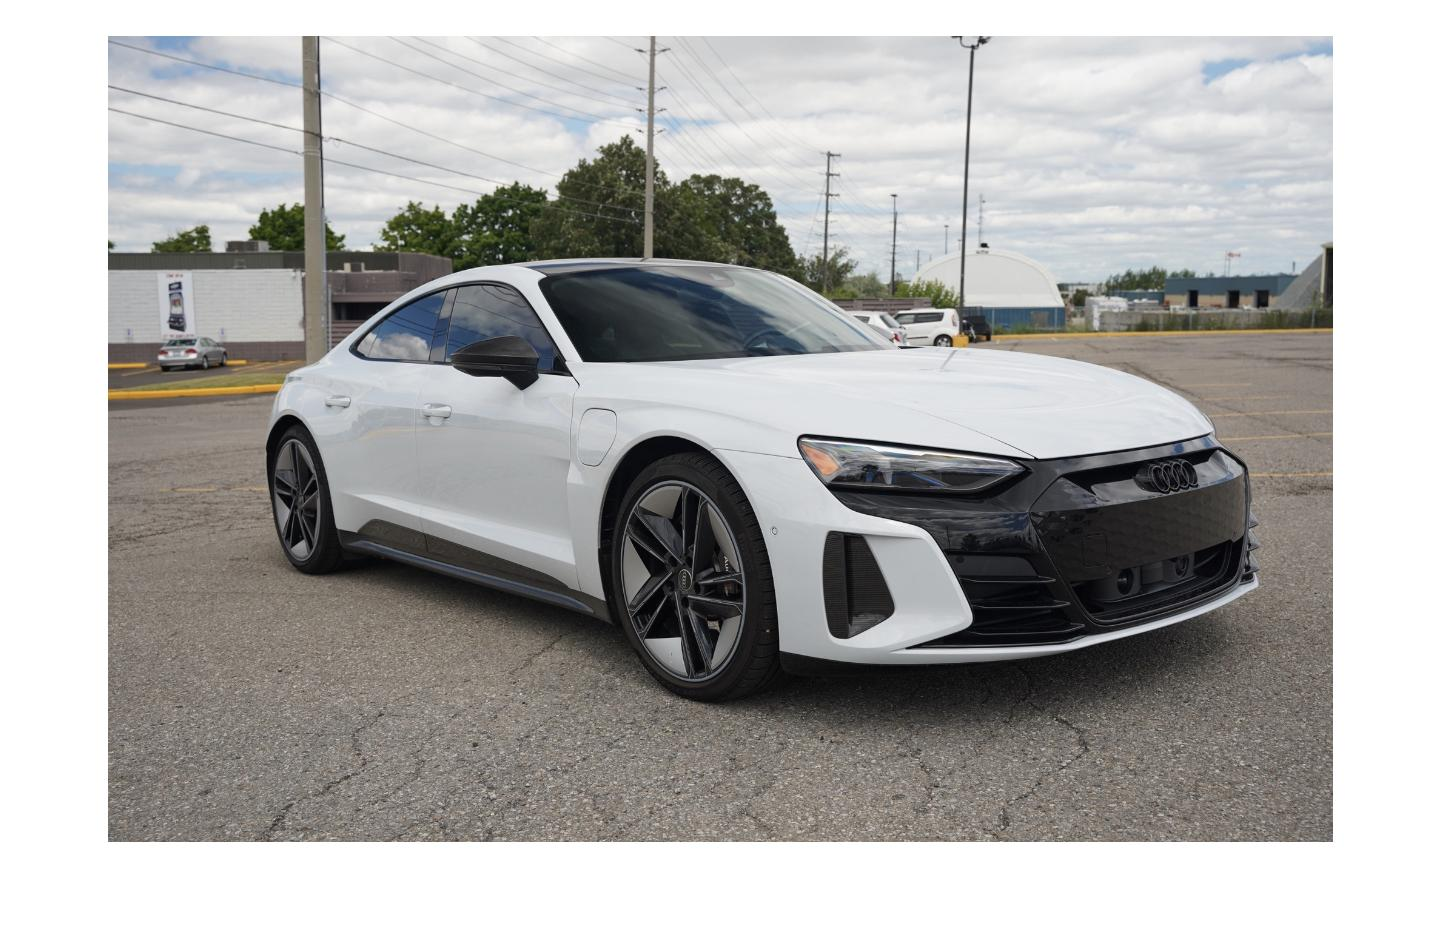
\includegraphics[width=\linewidth]{images/original.jpg}
\caption{Original image}
\end{subfigure}
\begin{subfigure}[b]{0.3\linewidth}
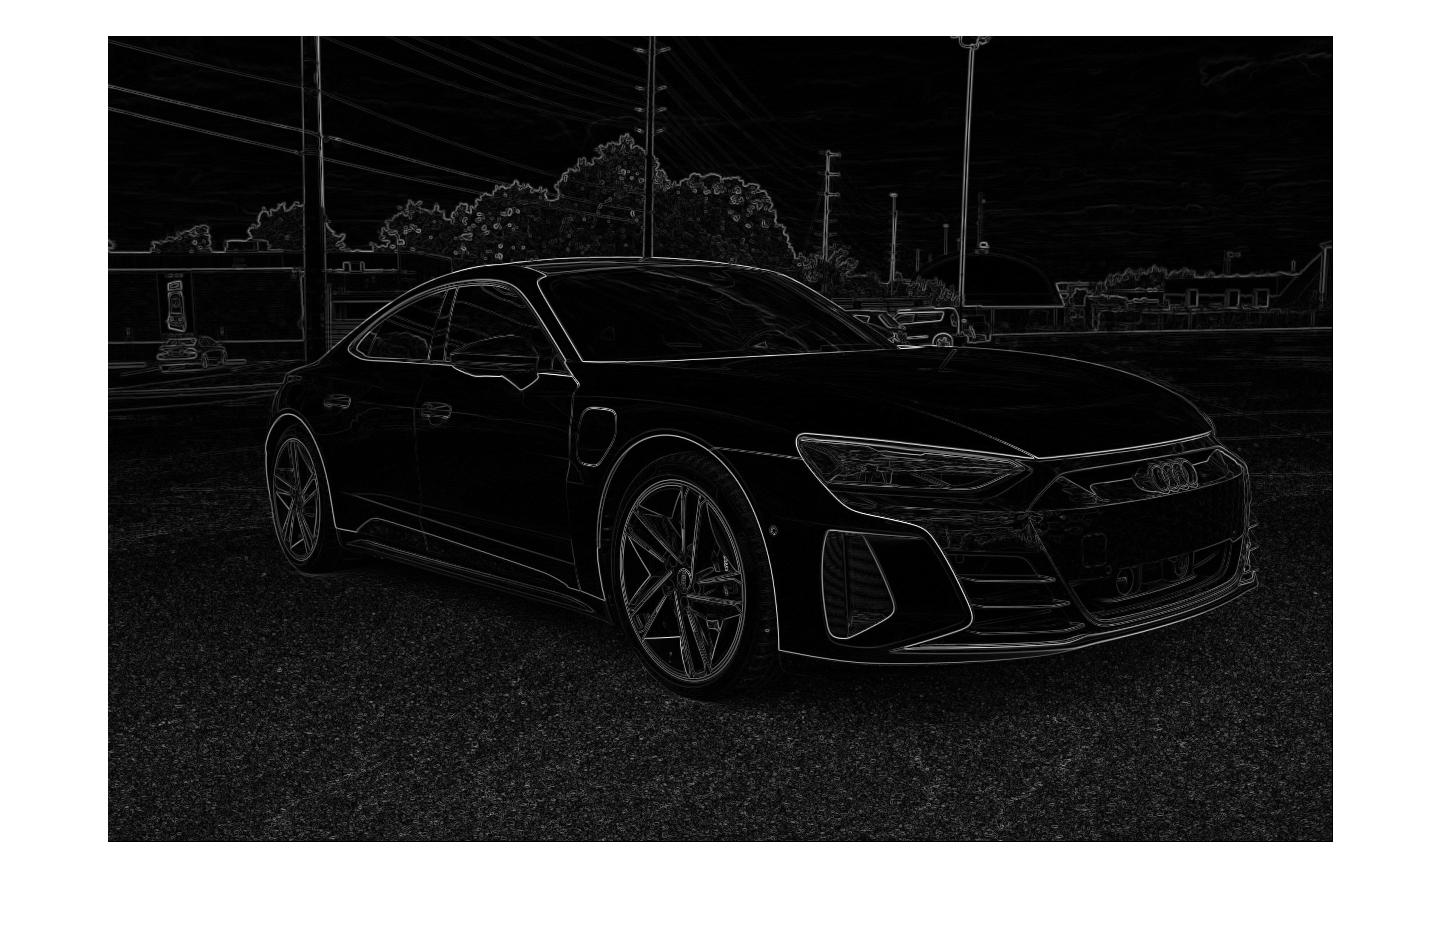
\includegraphics[width=\linewidth]{images/img1.jpg}
\caption{Filtered image}
\end{subfigure}
\begin{subfigure}[b]{0.3\linewidth}
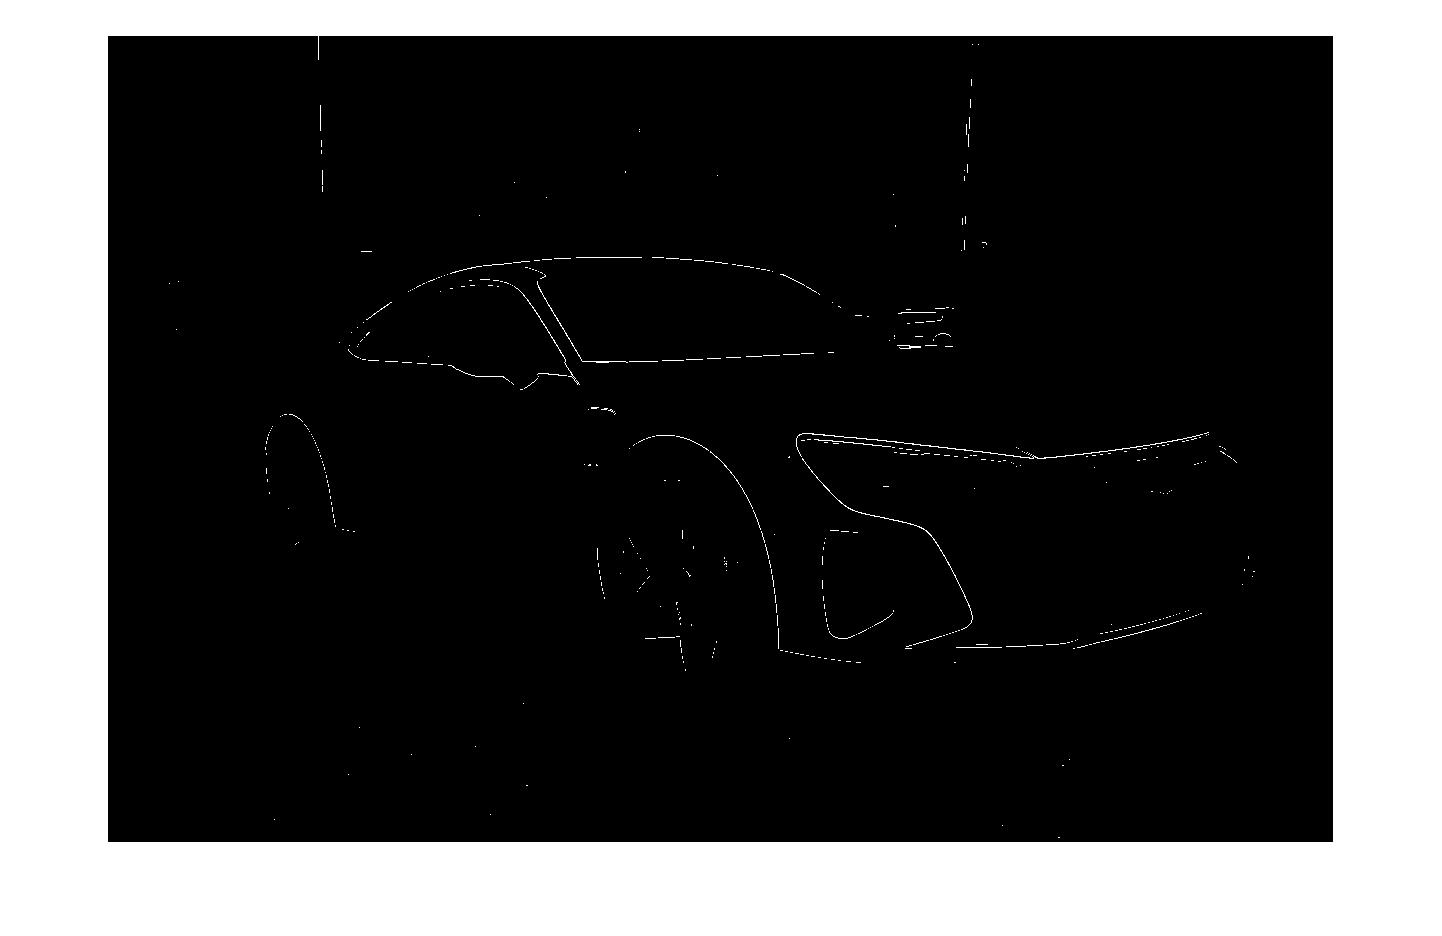
\includegraphics[width=\linewidth]{images/img2.jpg}
\caption{Edge detection}
\end{subfigure}
\caption{Roberts edge detection}
\label{fig:robert edge}
\end{figure}

The advantage of Robert operator is that it detect edges and orientation are very easy. Additionally, diagonal direction points are preserved. However, this operation is very sensitive to noise and not very accurate in edge detection. 

\clearpage

\textbf{2. Prewitt edge detector}
\newline

Prewitt operator computes the gradient approximation of image intensity function for image edge detection. At the pixels of an image, it produces either the normal to a vector or the corresponding gradient vector. It uses two 3 x 3 kernels or masks which are convolved with the input image to calculate approximations of the derivatives – one for horizontal changes, and one for vertical,

\[ M_x = 
\begin{bmatrix}
-1 & 0 & 1\\
-2 & 0 & 2\\
-1 & 0 & 1
\end{bmatrix}, 
M_y = 
\begin{bmatrix}
-1 & -1 & -1\\
0 & 0 & 0\\
1 & 1 & 1
\end{bmatrix}
\]

\begin{lstlisting}[language=Matlab]

% Assignment 2
% Part 1
% P1

% Load the original image
img = imread('/lamnguyen/Desktop/School/
Computer-Vision/A2/images/etronGTRS.jpg');

% Displaying Input Image
img = uint8(img);
figure; 
imshow(img); 

% Convert the image to grayscale
gray_img = rgb2gray(img);

% Convert the image to double
double_img = double(gray_img);
  
% Pre-allocate the filtered_image 
% matrix with zeros
filtered_img = zeros(size(double_img));

% Prewitt Operator Mask
Mx = [-1 0 1; -1 0 1; -1 0 1];
My = [-1 -1 -1; 0 0 0; 1 1 1];

% Edge Detection Process
% When i = 1 and j = 1, then filtered_image 
% pixel position will be filtered_image(2,2)
% The mask is of 3x3, so need to traverse
% to filtered_image(size(input_image, 1)-2,
% size(input_image, 2) - 2)
% Thus we are not considering the borders.
for i = 1:size(double_img, 1) - 2
 for j = 1:size(double_img, 2) - 2

 % Gradient approximations
 Gx=sum(sum(Mx.*double_img(i:i+2, j:j+2)));
 Gy=sum(sum(My.*double_img(i:i+2, j:j+2)));
				
 % Calculate magnitude of vector
 filtered_img(i+1, j+1)=sqrt(Gx.^2+Gy.^2);
		
 end
end

% Displaying Filtered Image
filtered_img = uint8(filtered_img);
figure;
imshow(filtered_img);
  
% Define a threshold value
thresholdValue = 100; % varies between [0 255]
prewitt_img = max(filtered_img, thresholdValue);
prewitt_img(prewitt_img == 
round(thresholdValue)) = 0;
  
% Displaying Output Image
prewitt_img = im2bw(prewitt_img);
figure;
imshow(prewitt_img); 

\end{lstlisting}

\begin{figure}[h!]
\centering
\begin{subfigure}[b]{0.3\linewidth}
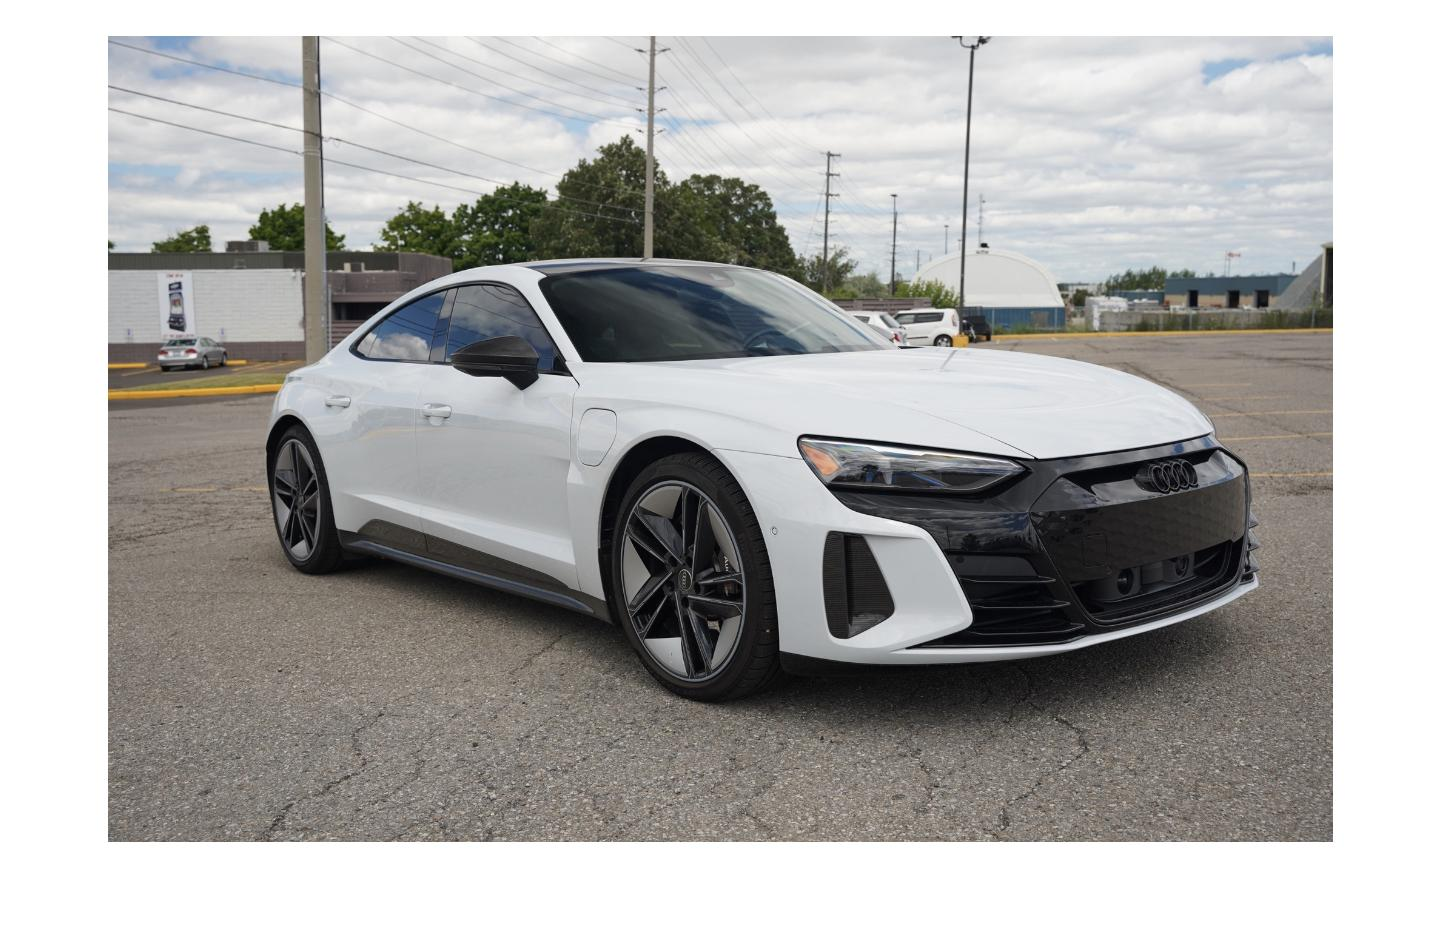
\includegraphics[width=\linewidth]{images/original.jpg}
\caption{Original image}
\end{subfigure}
\begin{subfigure}[b]{0.3\linewidth}
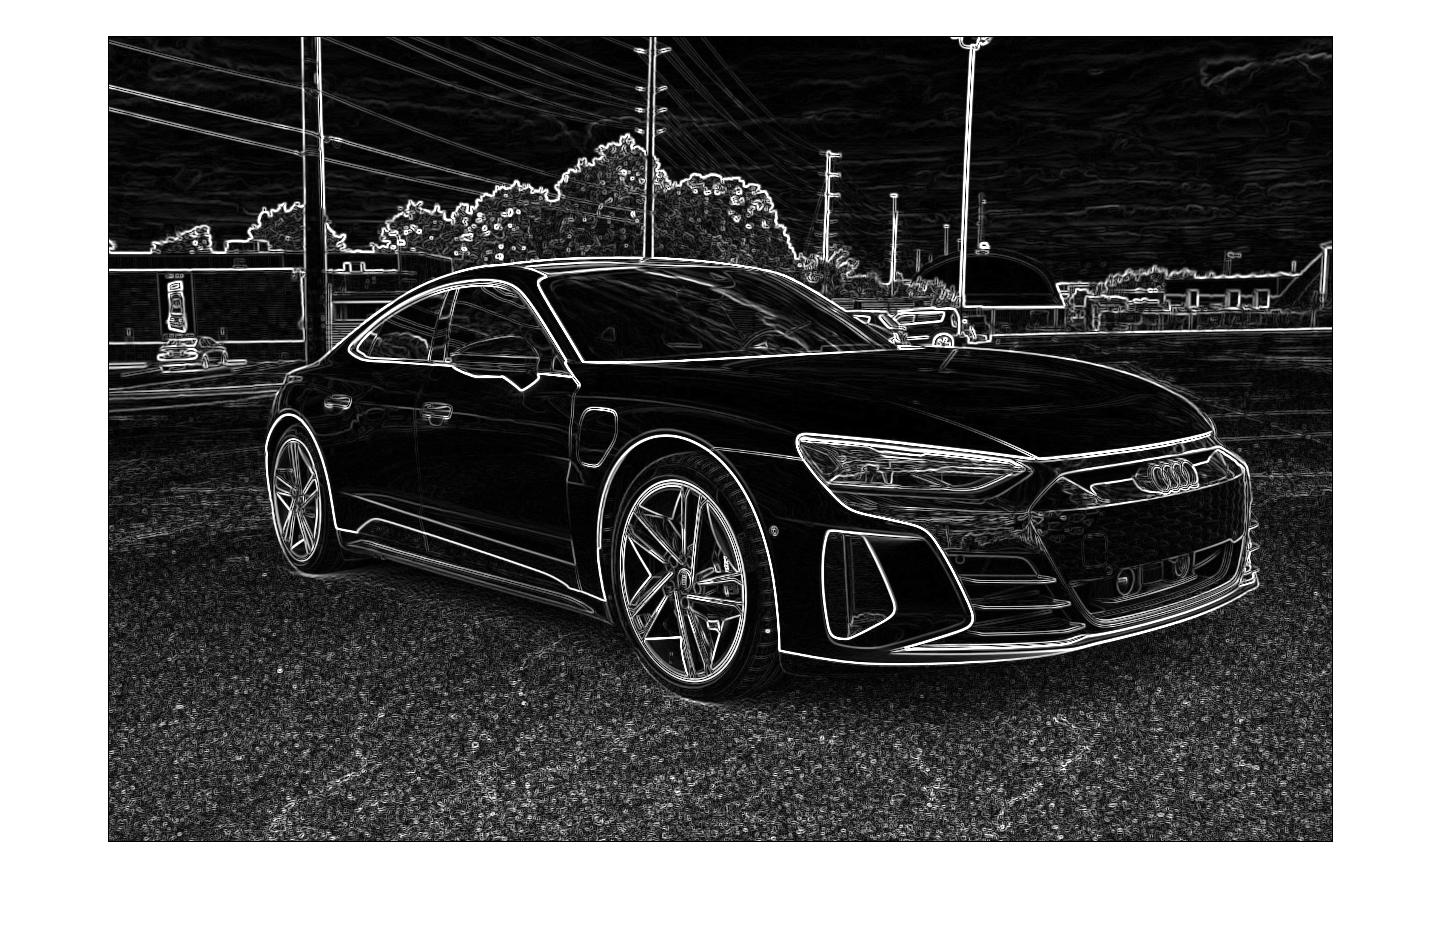
\includegraphics[width=\linewidth]{images/img3.jpg}
\caption{Filtered image}
\end{subfigure}
\begin{subfigure}[b]{0.3\linewidth}
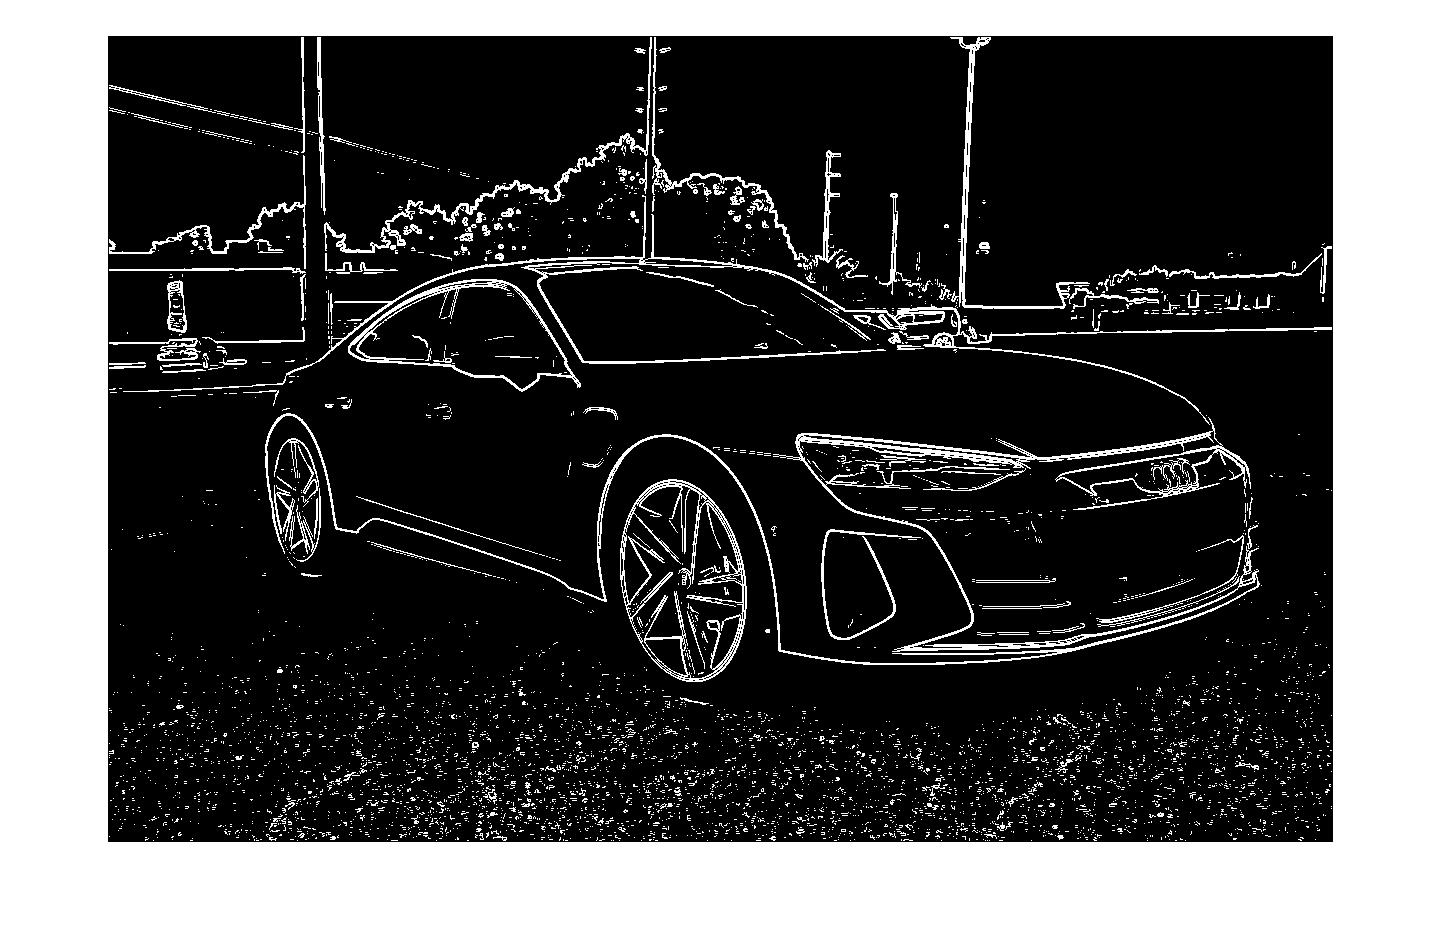
\includegraphics[width=\linewidth]{images/img4.jpg}
\caption{Edge detection}
\end{subfigure}
\caption{Prewitt edge detection}
\label{fig:prewitt edge}
\end{figure}

Prewitt operator has good performance on detecting vertical and horizontal edges. It seems to be the best operator to detect the orientation of an image. On the other hand, its limitation is that the magnitude of coefficient is fixed (cannot be changed) and diagonal direction points are not  always preserved.

\clearpage

\textbf{3. Sobel edge detector}
\newline

Sobel operator is a discrete differentiation gradient-based operator which a very similar to Prewitt operator. It also uses two 3 x 3 kernels or masks which are convolved with the input image to calculate the vertical and horizontal derivative approximations respectively, 

\[ M_x = 
\begin{bmatrix}
-1 & 0 & 1\\
-1 & 0 & 1\\
-1 & 0 & 1
\end{bmatrix}, 
M_y = 
\begin{bmatrix}
-1 & -2 & -1\\
0 & 0 & 0\\
1 & 2 & 1
\end{bmatrix}
\]

\begin{lstlisting}[language=Matlab]

% Assignment 2
% Part 1
% P1

% Load the original image
img = imread('/lamnguyen/Desktop/School/
Computer-Vision/A2/images/etronGTRS.jpg');

% Displaying Input Image
img = uint8(img);
figure; 
imshow(img); 

% Convert the image to grayscale
gray_img = rgb2gray(img);

% Convert the image to double
double_img = double(gray_img);
  
% Pre-allocate the filtered_image 
% matrix with zeros
filtered_img = zeros(size(double_img));

% Prewitt Operator Mask
Mx = [-1 0 1; -2 0 2; -1 0 1];
My = [-1 -2 -1; 0 0 0; 1 2 1];

% Edge Detection Process
% When i = 1 and j = 1, then filtered_image 
% pixel position will be filtered_image(2,2)
% The mask is of 3x3, so need to traverse
% to filtered_image(size(input_image, 1)-2,
% size(input_image, 2) - 2)
% Thus we are not considering the borders.
for i = 1:size(double_img, 1) - 2
 for j = 1:size(double_img, 2) - 2

 % Gradient approximations
 Gx=sum(sum(Mx.*double_img(i:i+2, j:j+2)));
 Gy=sum(sum(My.*double_img(i:i+2, j:j+2)));
				
 % Calculate magnitude of vector
 filtered_img(i+1, j+1)=sqrt(Gx.^2+Gy.^2);
		
 end
end

% Displaying Filtered Image
filtered_img = uint8(filtered_img);
figure;
imshow(filtered_img);
  
% Define a threshold value
thresholdValue = 100; % varies between [0 255]
sobel_img = max(filtered_img, thresholdValue);
sobel_img(sobel_img == 
round(thresholdValue)) = 0;
  
% Displaying Output Image
sobel_img = im2bw(sobel_img);
figure;
imshow(sobel_img);  

\end{lstlisting}

\begin{figure}[h!]
\centering
\begin{subfigure}[b]{0.3\linewidth}
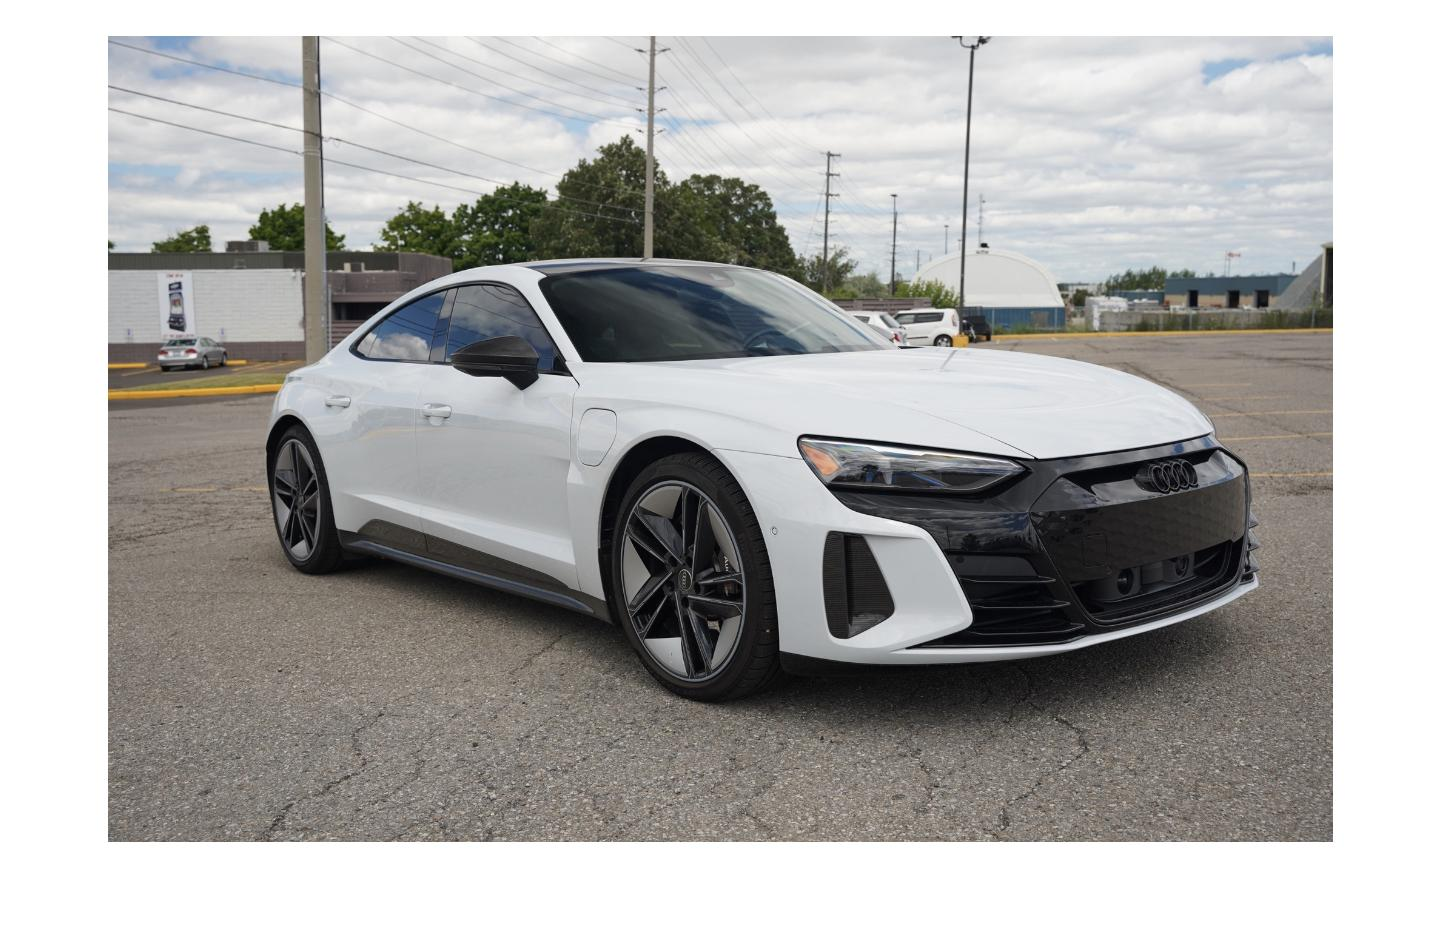
\includegraphics[width=\linewidth]{images/original.jpg}
\caption{Original image}
\end{subfigure}
\begin{subfigure}[b]{0.3\linewidth}
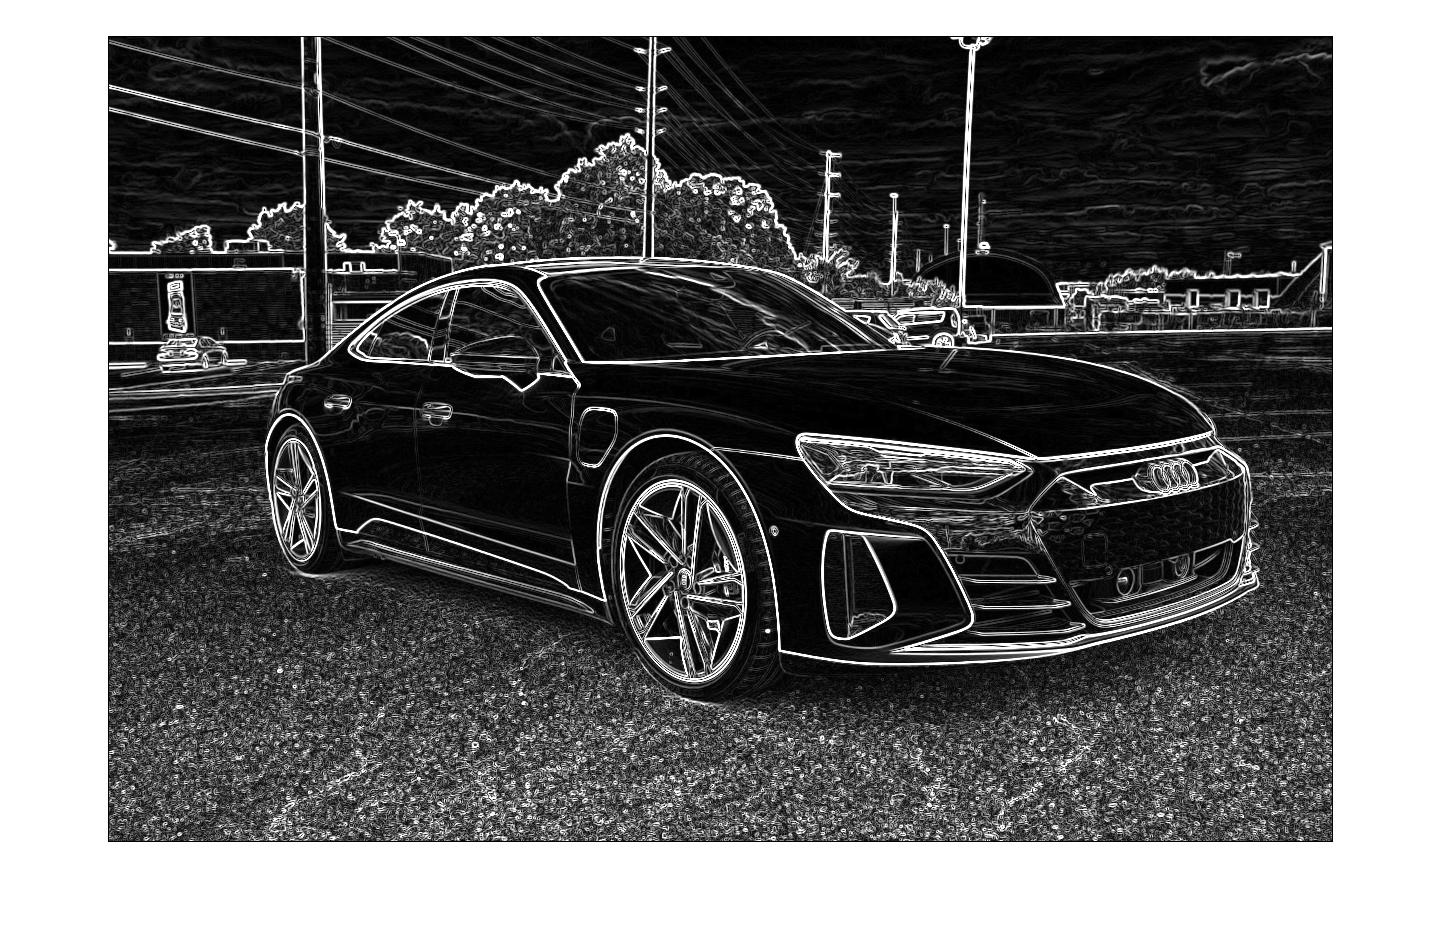
\includegraphics[width=\linewidth]{images/img5.jpg}
\caption{Filtered image}
\end{subfigure}
\begin{subfigure}[b]{0.3\linewidth}
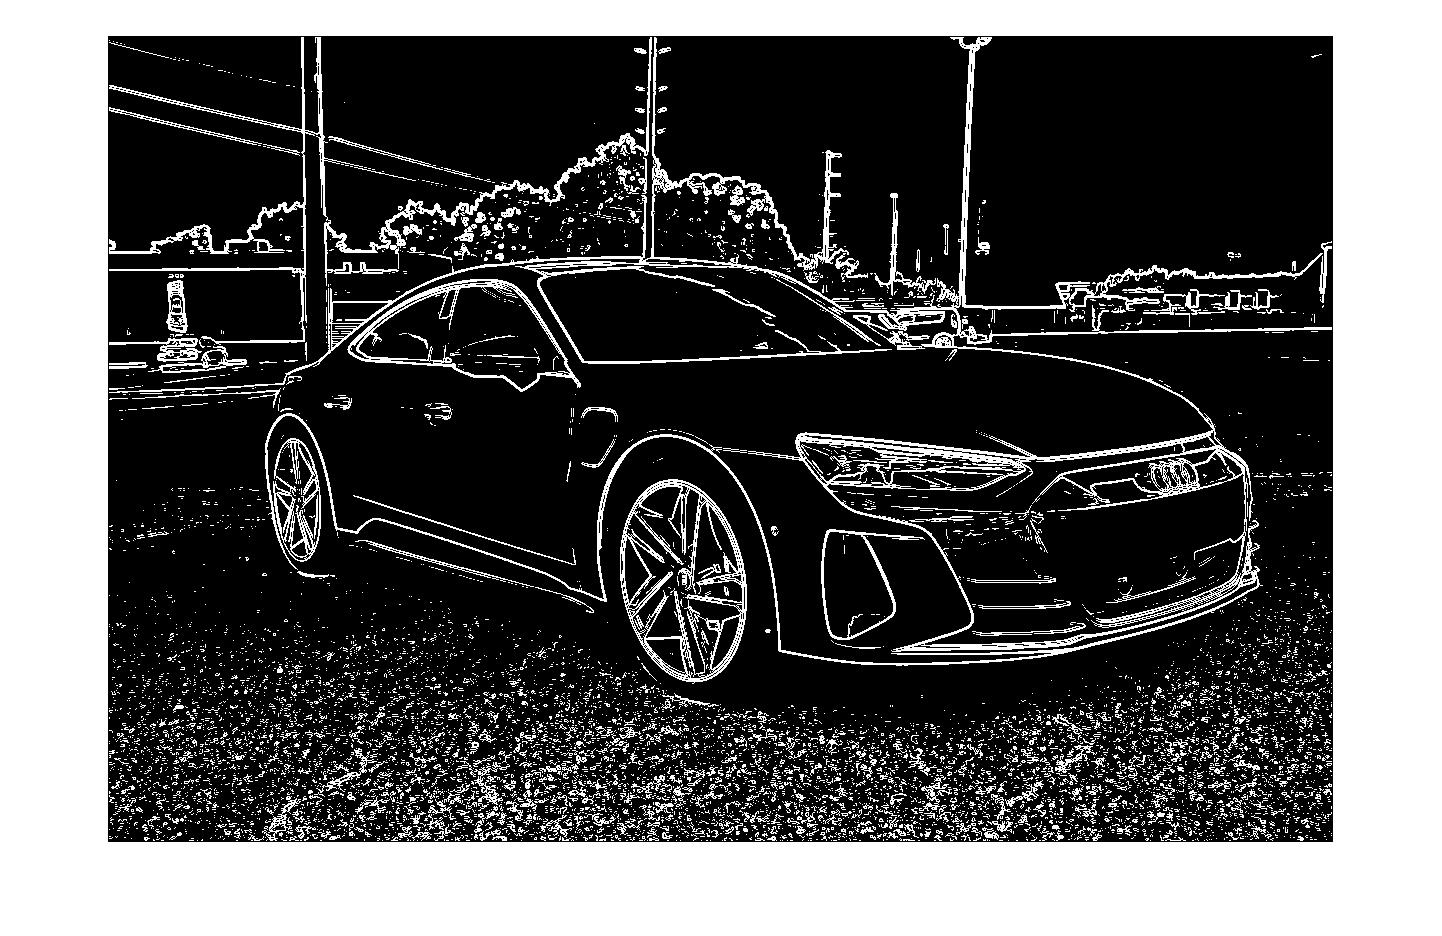
\includegraphics[width=\linewidth]{images/img6.jpg}
\caption{Edge detection}
\end{subfigure}
\caption{Sobel edge detection}
\label{fig:sobel edge}
\end{figure}

Sobel operator is simple and efficient in terms of time computation. Moreover, it is very easy at searching for smooth edges. However, this technique has some drawbacks such as diagonal direction points are not preserved always, sensitive to noise, not very accurate in edge detection, and thick and rough edges detection does not give appropriate results.

\clearpage

\subsection{Problem 2}

The \(1^{st}\) derivative function of an 1D image as function \(f(x)\) is 

\[ {\frac{\partial f}{\partial x}} = f(x + 1) - f(x) \]

The \(2^{nd}\) derivative function is as follow 

\[ {\frac{\partial^2 f}{\partial x^2}} = f(x + 1) + f(x - 1)- 2f(x) \]

Given 1D image \(f(x)\) as below

\begin{figure}[h!]
\centering
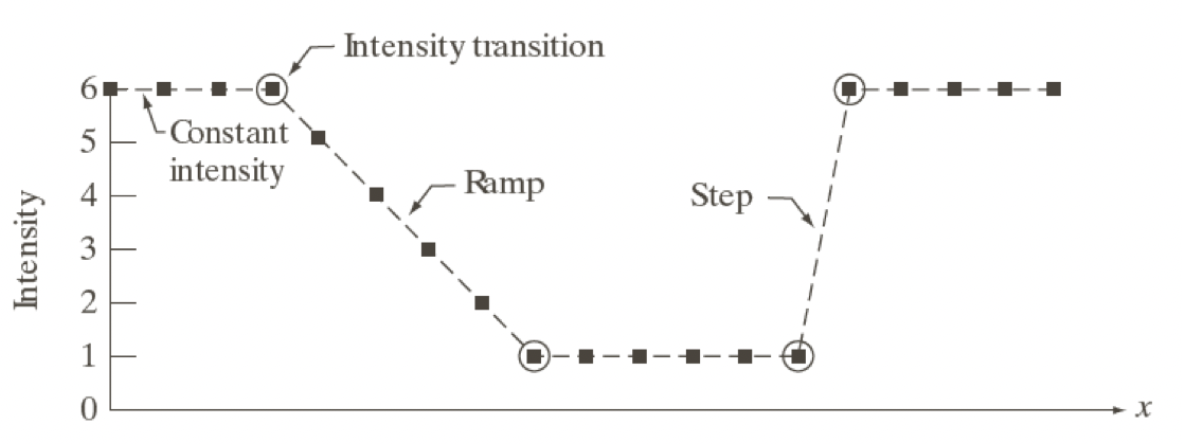
\includegraphics[width=0.8\linewidth]{images/img.jpg}
\caption{1D image}
\label{fig:1D image}
\end{figure}

Scan line \\
\begin{tabularx}{0.5\textwidth} { 
  | >{\centering\arraybackslash}X
  | >{\centering\arraybackslash}X
  | >{\centering\arraybackslash}X 
  | >{\centering\arraybackslash}X
  | >{\centering\arraybackslash}X
  | >{\centering\arraybackslash}X
  | >{\centering\arraybackslash}X
  | >{\centering\arraybackslash}X
  | >{\centering\arraybackslash}X
  | >{\centering\arraybackslash}X
  | >{\centering\arraybackslash}X
  | >{\centering\arraybackslash}X
  | >{\centering\arraybackslash}X
  | >{\centering\arraybackslash}X
  | >{\centering\arraybackslash}X
  | >{\centering\arraybackslash}X
  | >{\centering\arraybackslash}X
  | >{\centering\arraybackslash}X
  | >{\centering\arraybackslash}X | }
 \hline
 6 & 6 & 6 & 6 & 5 & 4 & 3 & 2 & 1 & 1 & 1 & 1 & 1 & 1 & 6 & 6 & 6 & 6 & 6\\
\hline
\end{tabularx} \\

Sample calculation for \(1^{st}\) order derivative
\[ {\frac{\partial f}{\partial x}} = f(x + 1) - f(x) = 6 - 6 = 0\]
\(1^{st}\) derivative \\ 
\begin{tabularx}{0.7\textwidth} { 
  | >{\centering\arraybackslash}X
  | >{\centering\arraybackslash}X
  | >{\centering\arraybackslash}X 
  | >{\centering\arraybackslash}X
  | >{\centering\arraybackslash}X
  | >{\centering\arraybackslash}X
  | >{\centering\arraybackslash}X
  | >{\centering\arraybackslash}X
  | >{\centering\arraybackslash}X
  | >{\centering\arraybackslash}X
  | >{\centering\arraybackslash}X
  | >{\centering\arraybackslash}X
  | >{\centering\arraybackslash}X
  | >{\centering\arraybackslash}X
  | >{\centering\arraybackslash}X
  | >{\centering\arraybackslash}X
  | >{\centering\arraybackslash}X
  | >{\centering\arraybackslash}X
  | >{\centering\arraybackslash}X | }
 \hline
  & 0 & 0 & \(-1\) & \(-1\) & \(-1\) & \(-1\) & \(-1\) & 0 & 0 & 0 & 0 & 0 & 5 & 0 & 0 & 0 & 0 & \\
\hline
\end{tabularx} \\

Sample calculation for \(2^{nd}\) order derivative
\[ {\frac{\partial^2 f}{\partial x^2}} = f(x + 1) + f(x - 1)- 2f(x) = 6 + 6 - 2*6 = 0\]

\(2^{nd}\) derivative \\ 
\begin{tabularx}{0.7\textwidth} { 
  | >{\centering\arraybackslash}X
  | >{\centering\arraybackslash}X
  | >{\centering\arraybackslash}X 
  | >{\centering\arraybackslash}X
  | >{\centering\arraybackslash}X
  | >{\centering\arraybackslash}X
  | >{\centering\arraybackslash}X
  | >{\centering\arraybackslash}X
  | >{\centering\arraybackslash}X
  | >{\centering\arraybackslash}X
  | >{\centering\arraybackslash}X
  | >{\centering\arraybackslash}X
  | >{\centering\arraybackslash}X
  | >{\centering\arraybackslash}X
  | >{\centering\arraybackslash}X
  | >{\centering\arraybackslash}X
  | >{\centering\arraybackslash}X
  | >{\centering\arraybackslash}X
  | >{\centering\arraybackslash}X | }
 \hline
  & 0 & 0 & \(-1\) & 0 & 0 & 0 & 0 & 1 & 0 & 0 & 0 & 0 & 5 & \(-5\) & 0 & 0 & 0 & \\
\hline
\end{tabularx} \\

\clearpage
\subsection{Problem 3}

The image sharpening process based on unsharp masking and high-boost filtering:
\begin{description}[font=$\bullet$~\normalfont\scshape\color{red!50!black}]
  \item Blur the original image
  \item Subtract the blurred image from the original to get the mask
  \[ f_s(x, y) = f(x, y) - \overline{f}(x, y) \]
  \item Add the mask to the original image
  \[ g(x, y) = f(x, y) +  k*(f(x, y) - \overline{f}(x, y)) \]
  \[ k \geq 0 \]
\end{description}

where \(k\) specifies what portion of mask to be added. When \[ k = 1 \] is known as unsharp masking. For \[ k > 1 \], we call this as high-boost filtering because we are boosting the high-frequency components by giving more weight to the mask (edge) image. 

\begin{lstlisting}[language=Matlab]

% Assignment 2
% Part 1
% P3

% Load the original image
img = imread('/lamnguyen/Desktop/School/
Computer-Vision/A2/images/friends.jpg');

% Displaying Input Image
img = uint8(img);
figure; 
imshow(img); 

% Convert the image to grayscale
gray_img = rgb2gray(img);
figure; 
imshow(gray_img);

% Filter the image with a Gaussian 
% filter with standard deviation of 5
blur_img = imgaussfilt(gray_img, 5);
figure; 
imshow(blur_img);

% Get the mask
mask = gray_img - blur_img;
figure; 
imshow(mask);

% Unsharp masking 
% Set k = 1
k = 1;
um_img = gray_img + k*mask;
figure; 
imshow(um_img);

% High-boost filtering
% Set k = 5
k = 5;
hb_img = gray_img + k*mask;
figure; 
imshow(hb_img);

\end{lstlisting}

\begin{figure}[h!]
\centering
\begin{subfigure}[b]{0.3\linewidth}
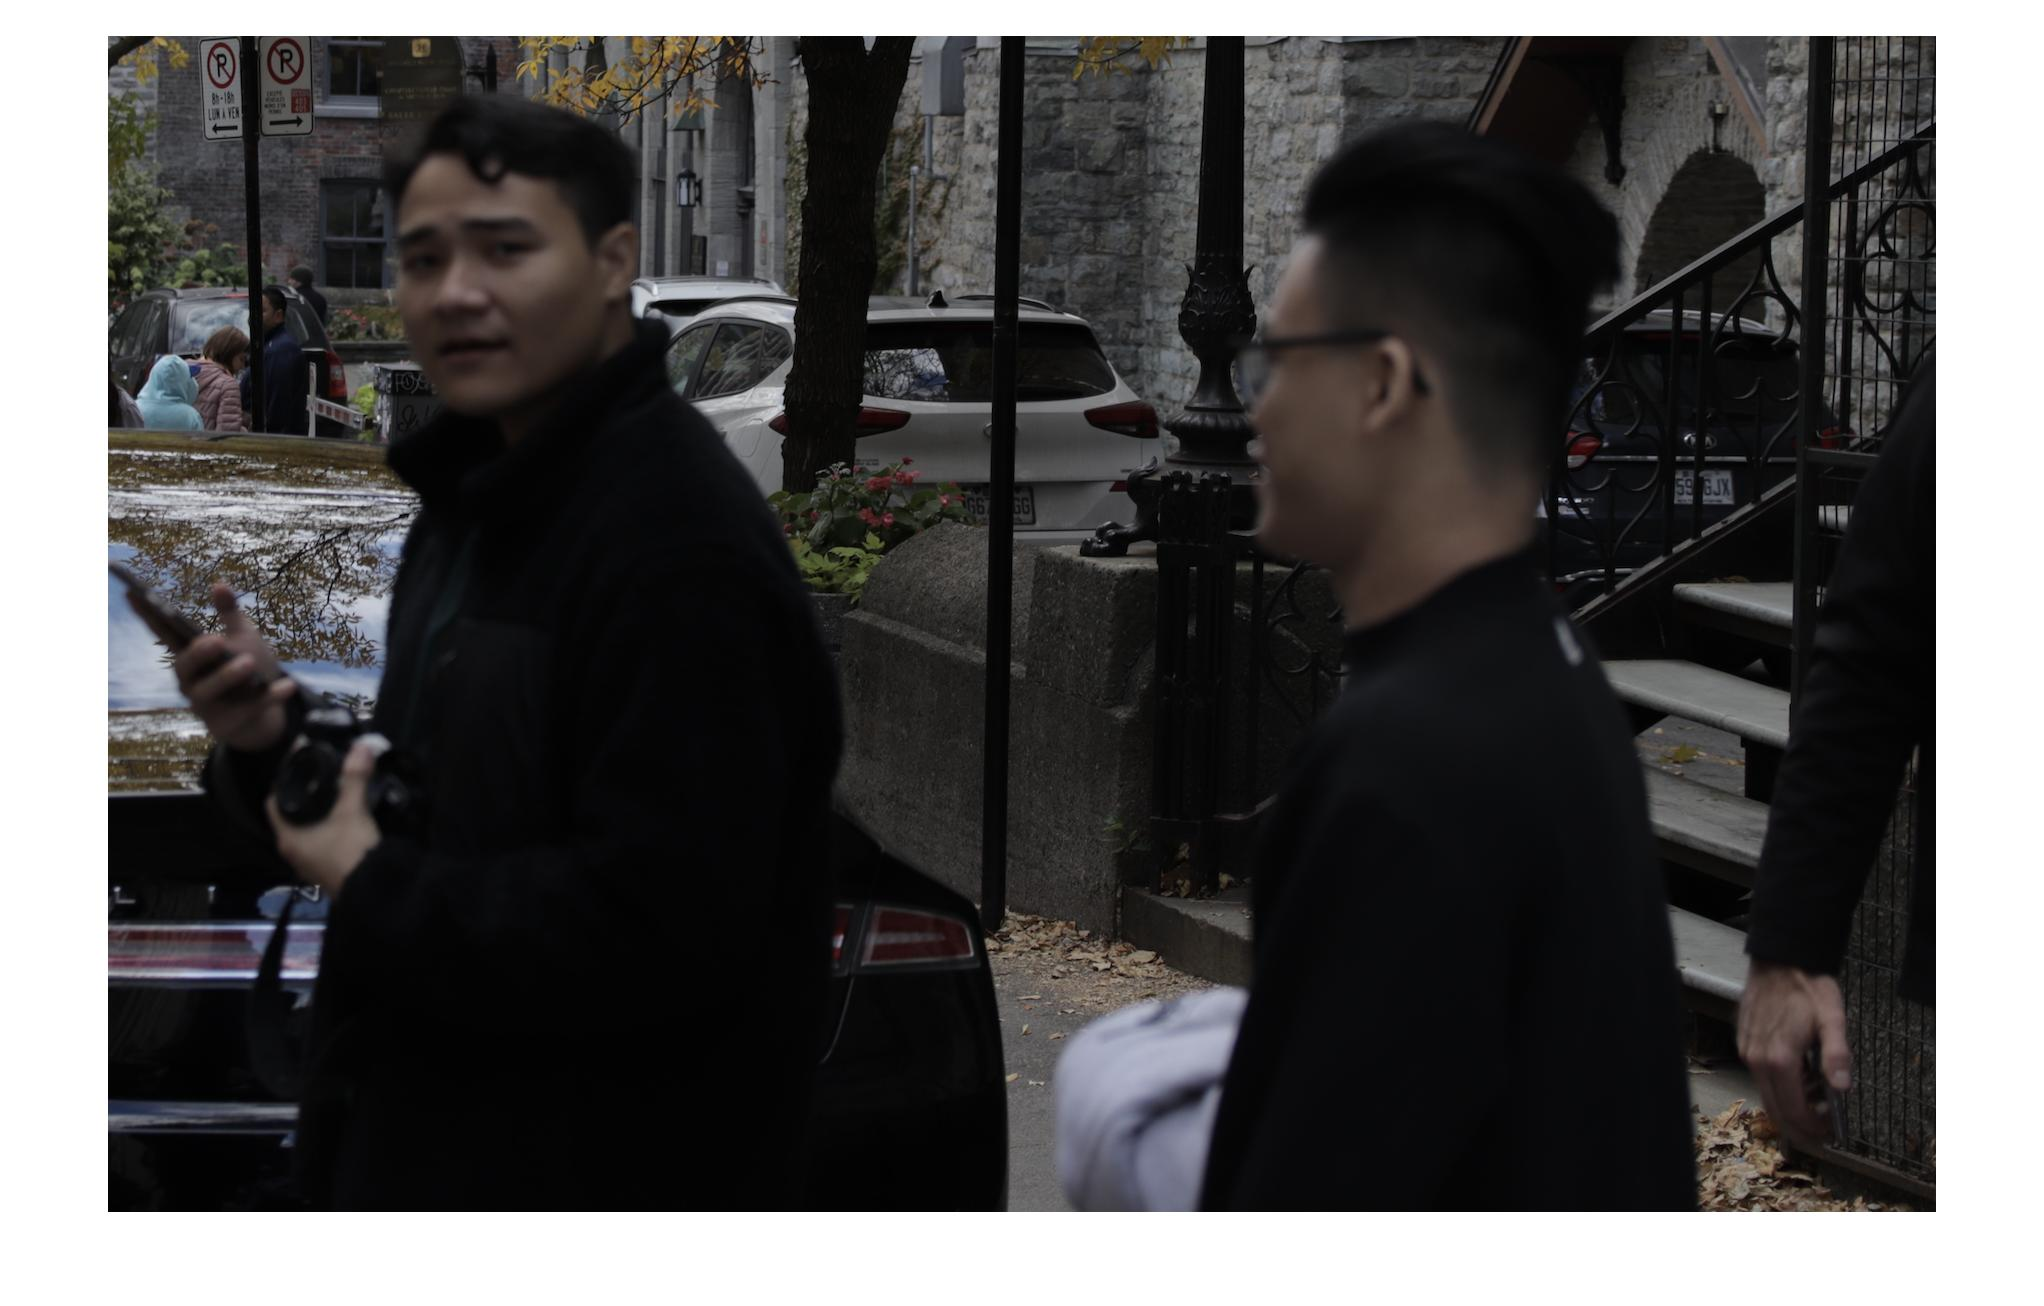
\includegraphics[width=\linewidth]{images/img7.jpg}
\caption{}
\end{subfigure}
\begin{subfigure}[b]{0.3\linewidth}
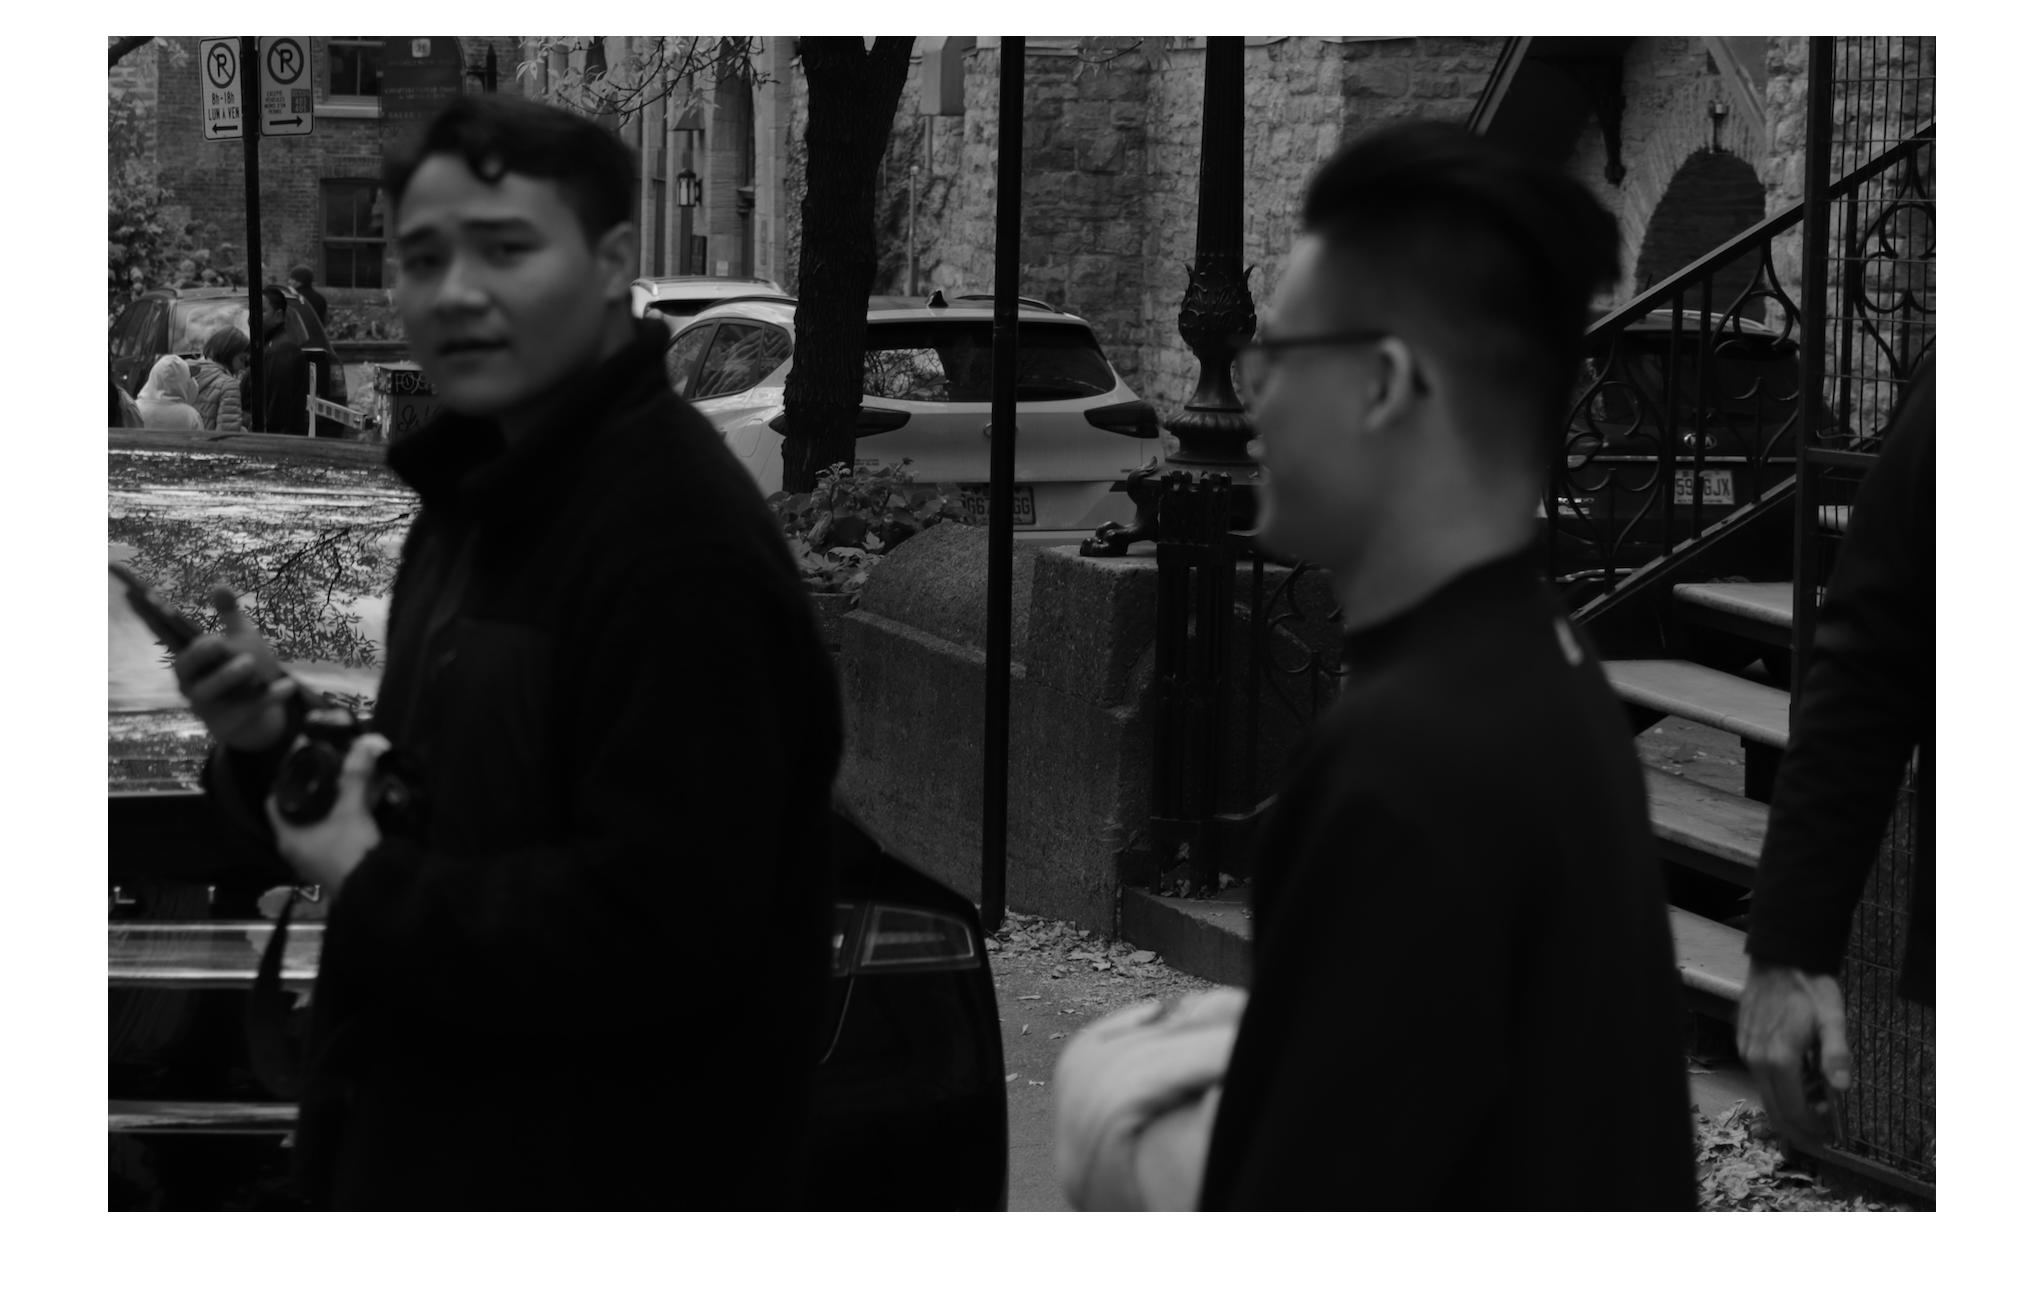
\includegraphics[width=\linewidth]{images/img8.jpg}
\caption{}
\end{subfigure}
\begin{subfigure}[b]{0.3\linewidth}
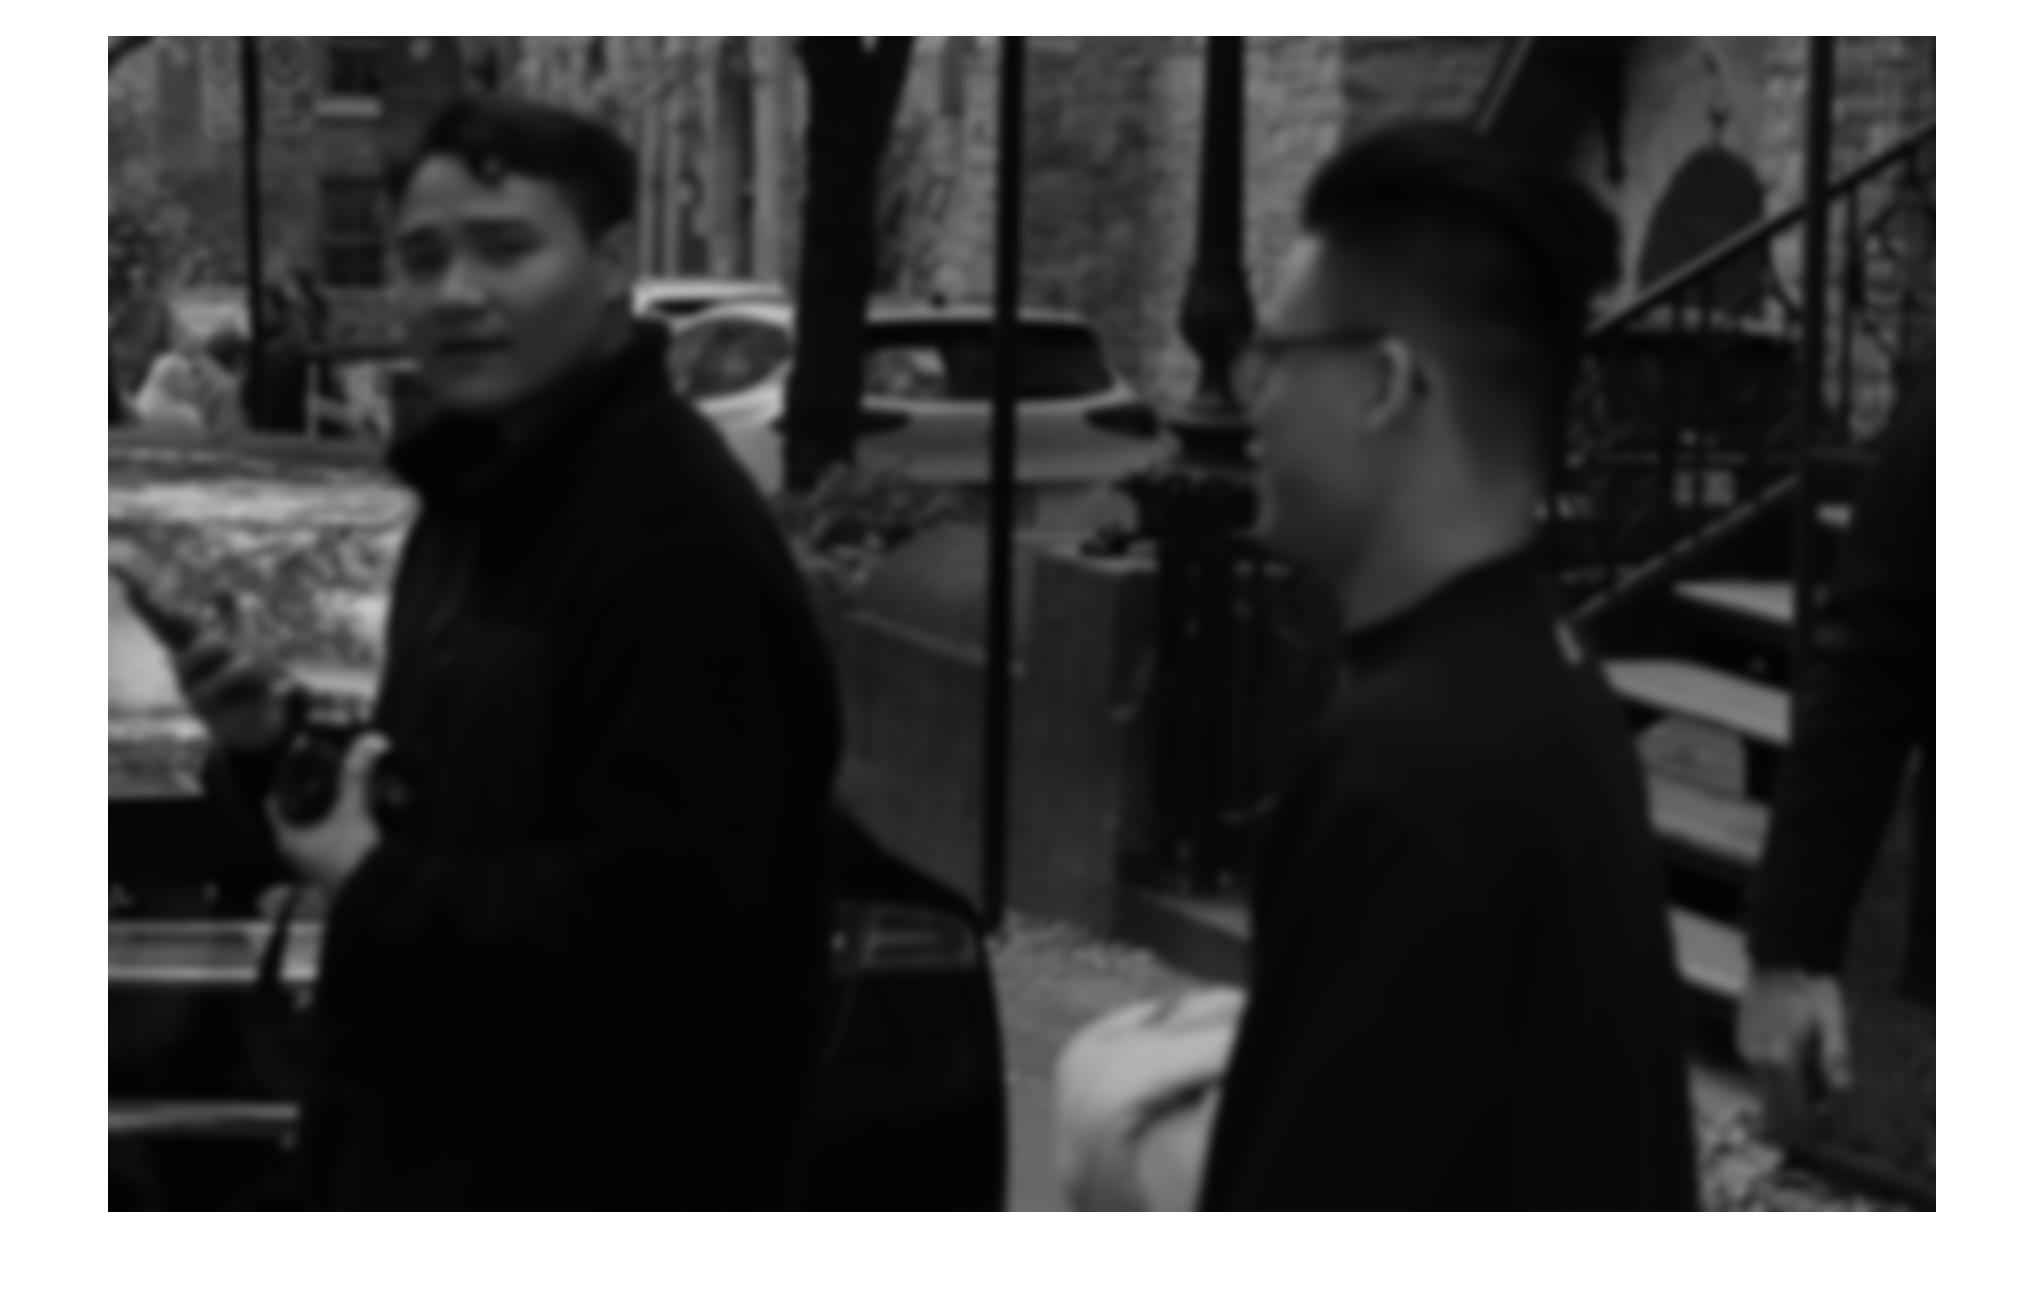
\includegraphics[width=\linewidth]{images/img9.jpg}
\caption{}
\end{subfigure}
\begin{subfigure}[b]{0.3\linewidth}
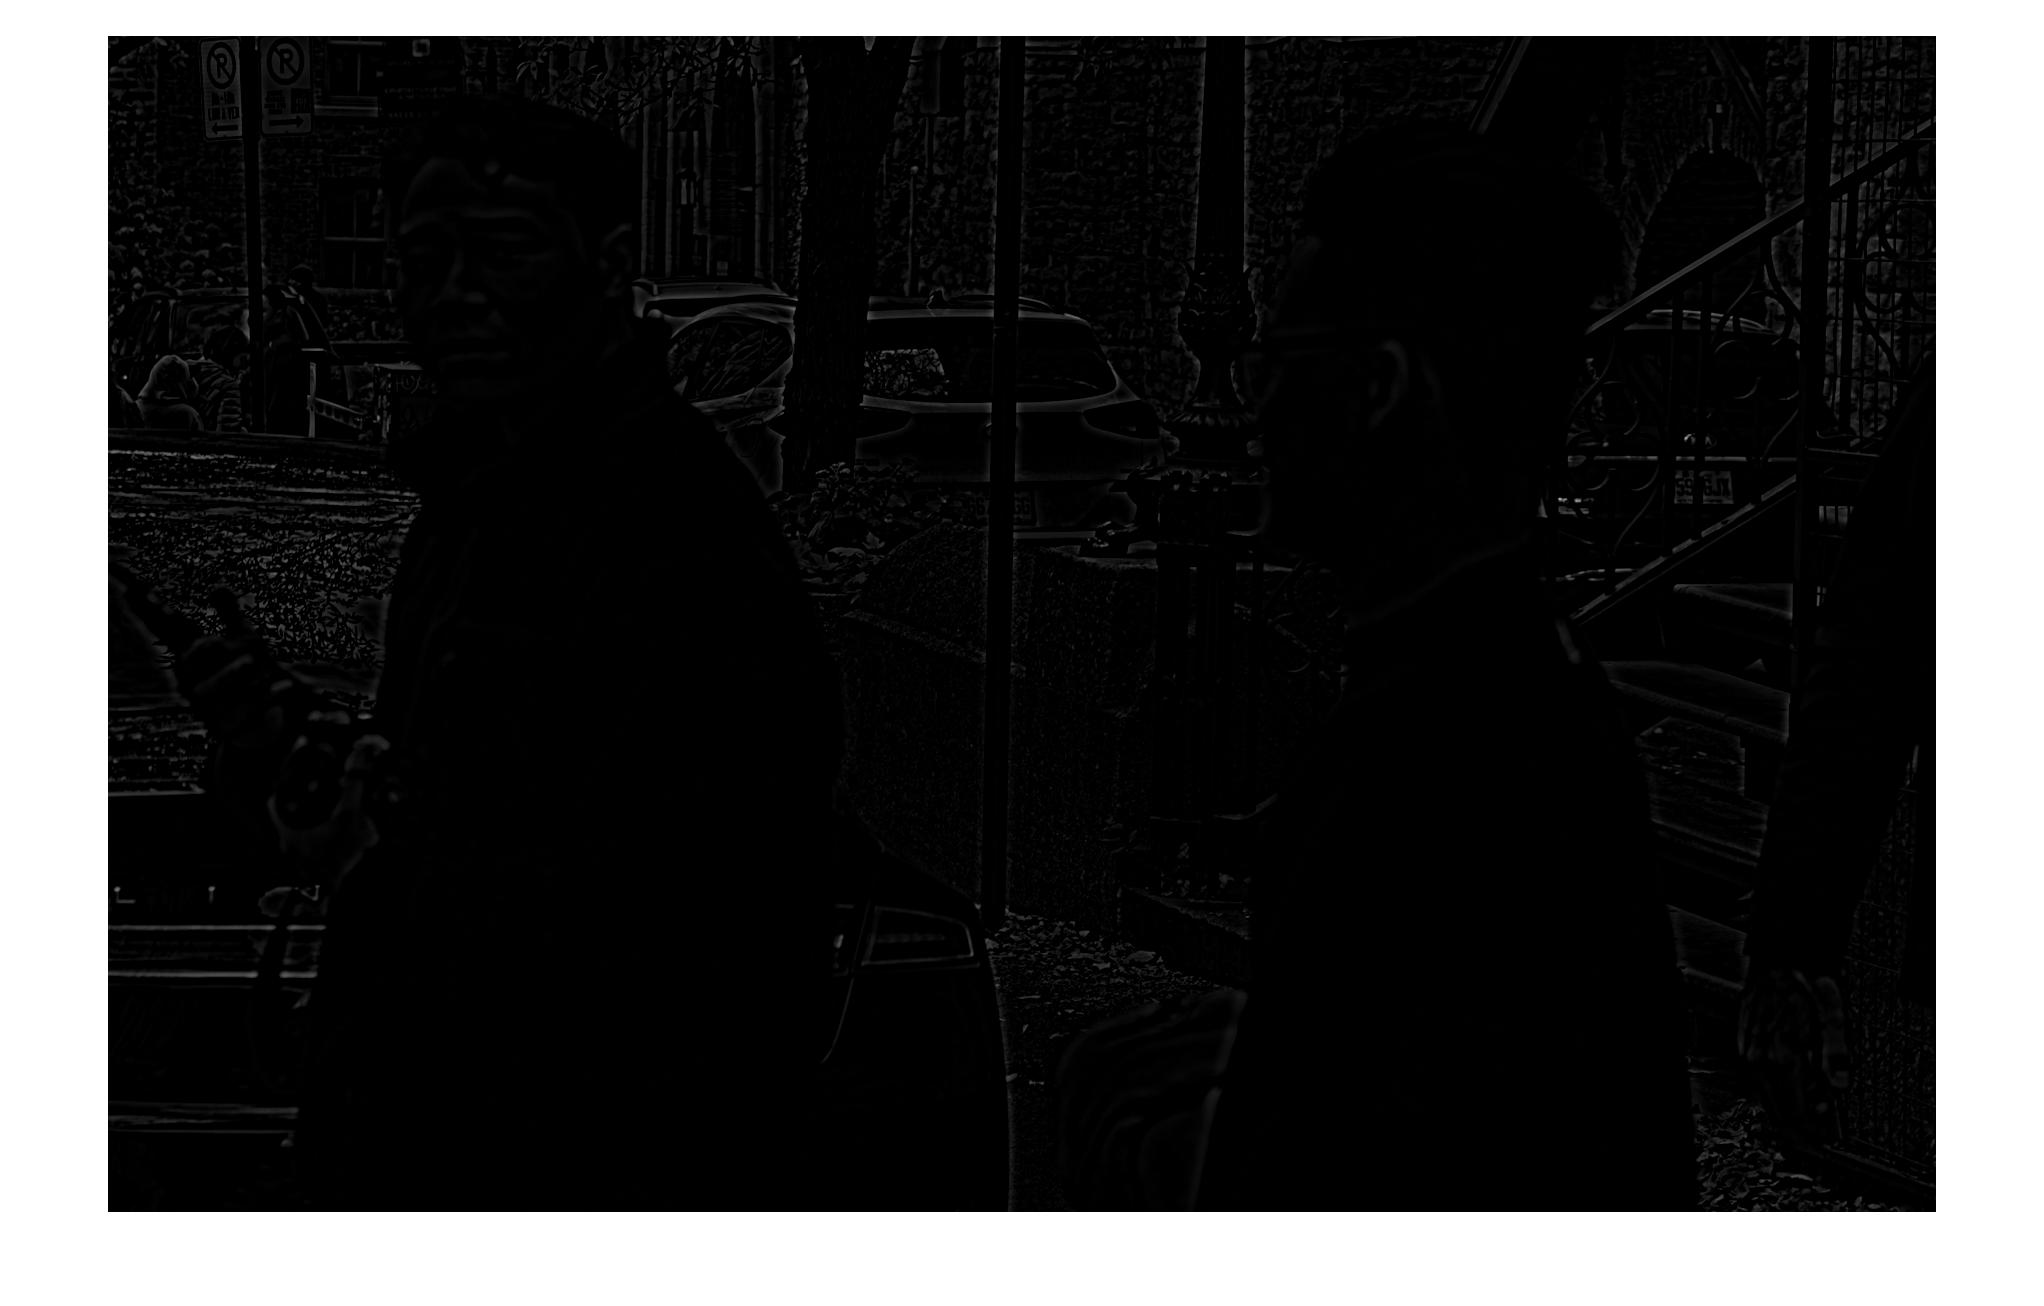
\includegraphics[width=\linewidth]{images/img10.jpg}
\caption{}
\end{subfigure}
\begin{subfigure}[b]{0.3\linewidth}
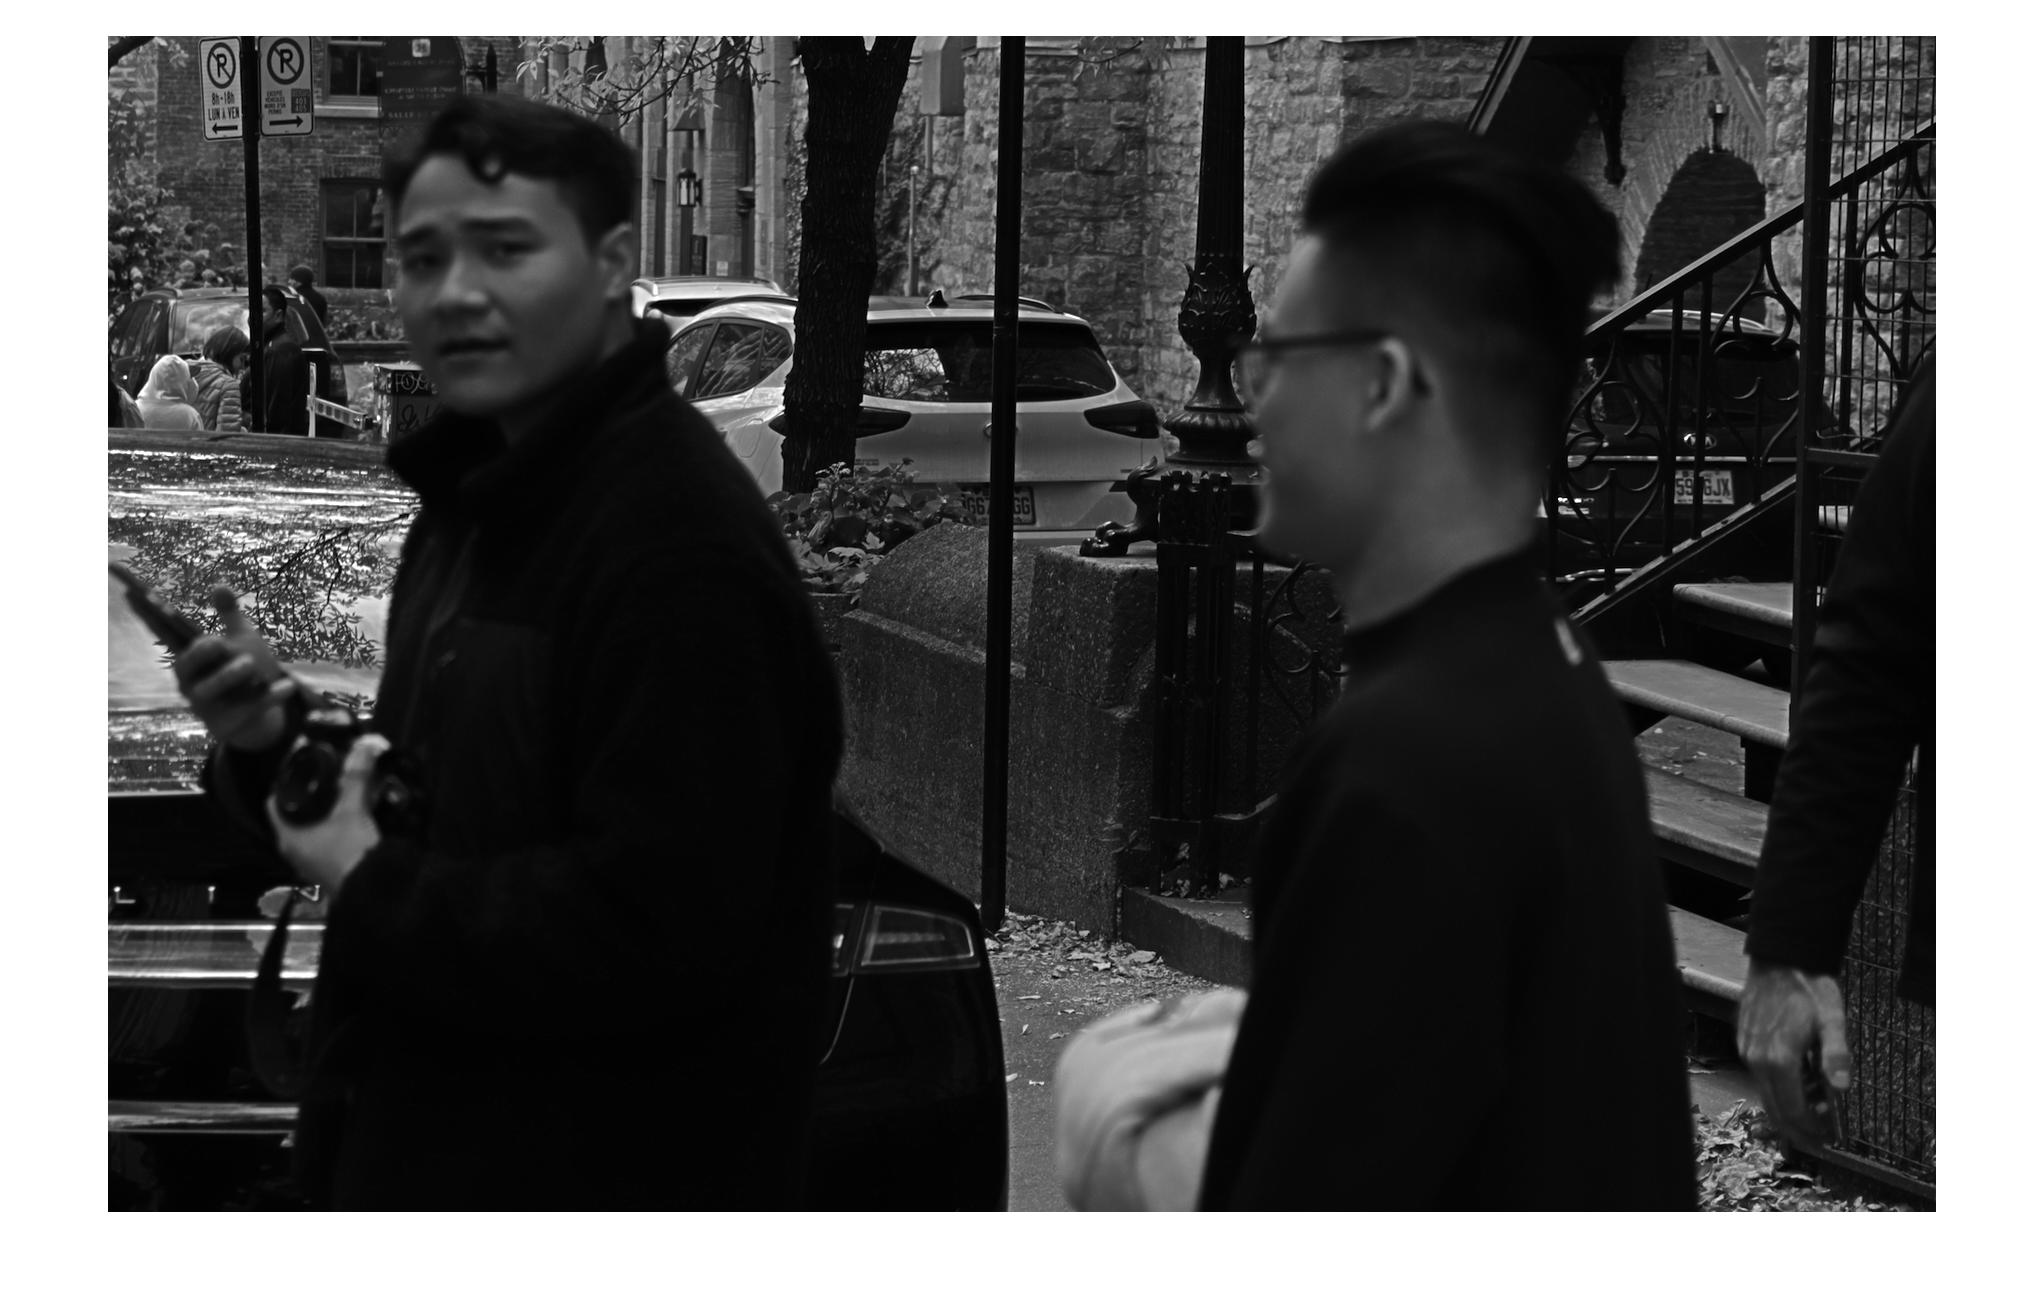
\includegraphics[width=\linewidth]{images/img11.jpg}
\caption{}
\end{subfigure}
\begin{subfigure}[b]{0.3\linewidth}
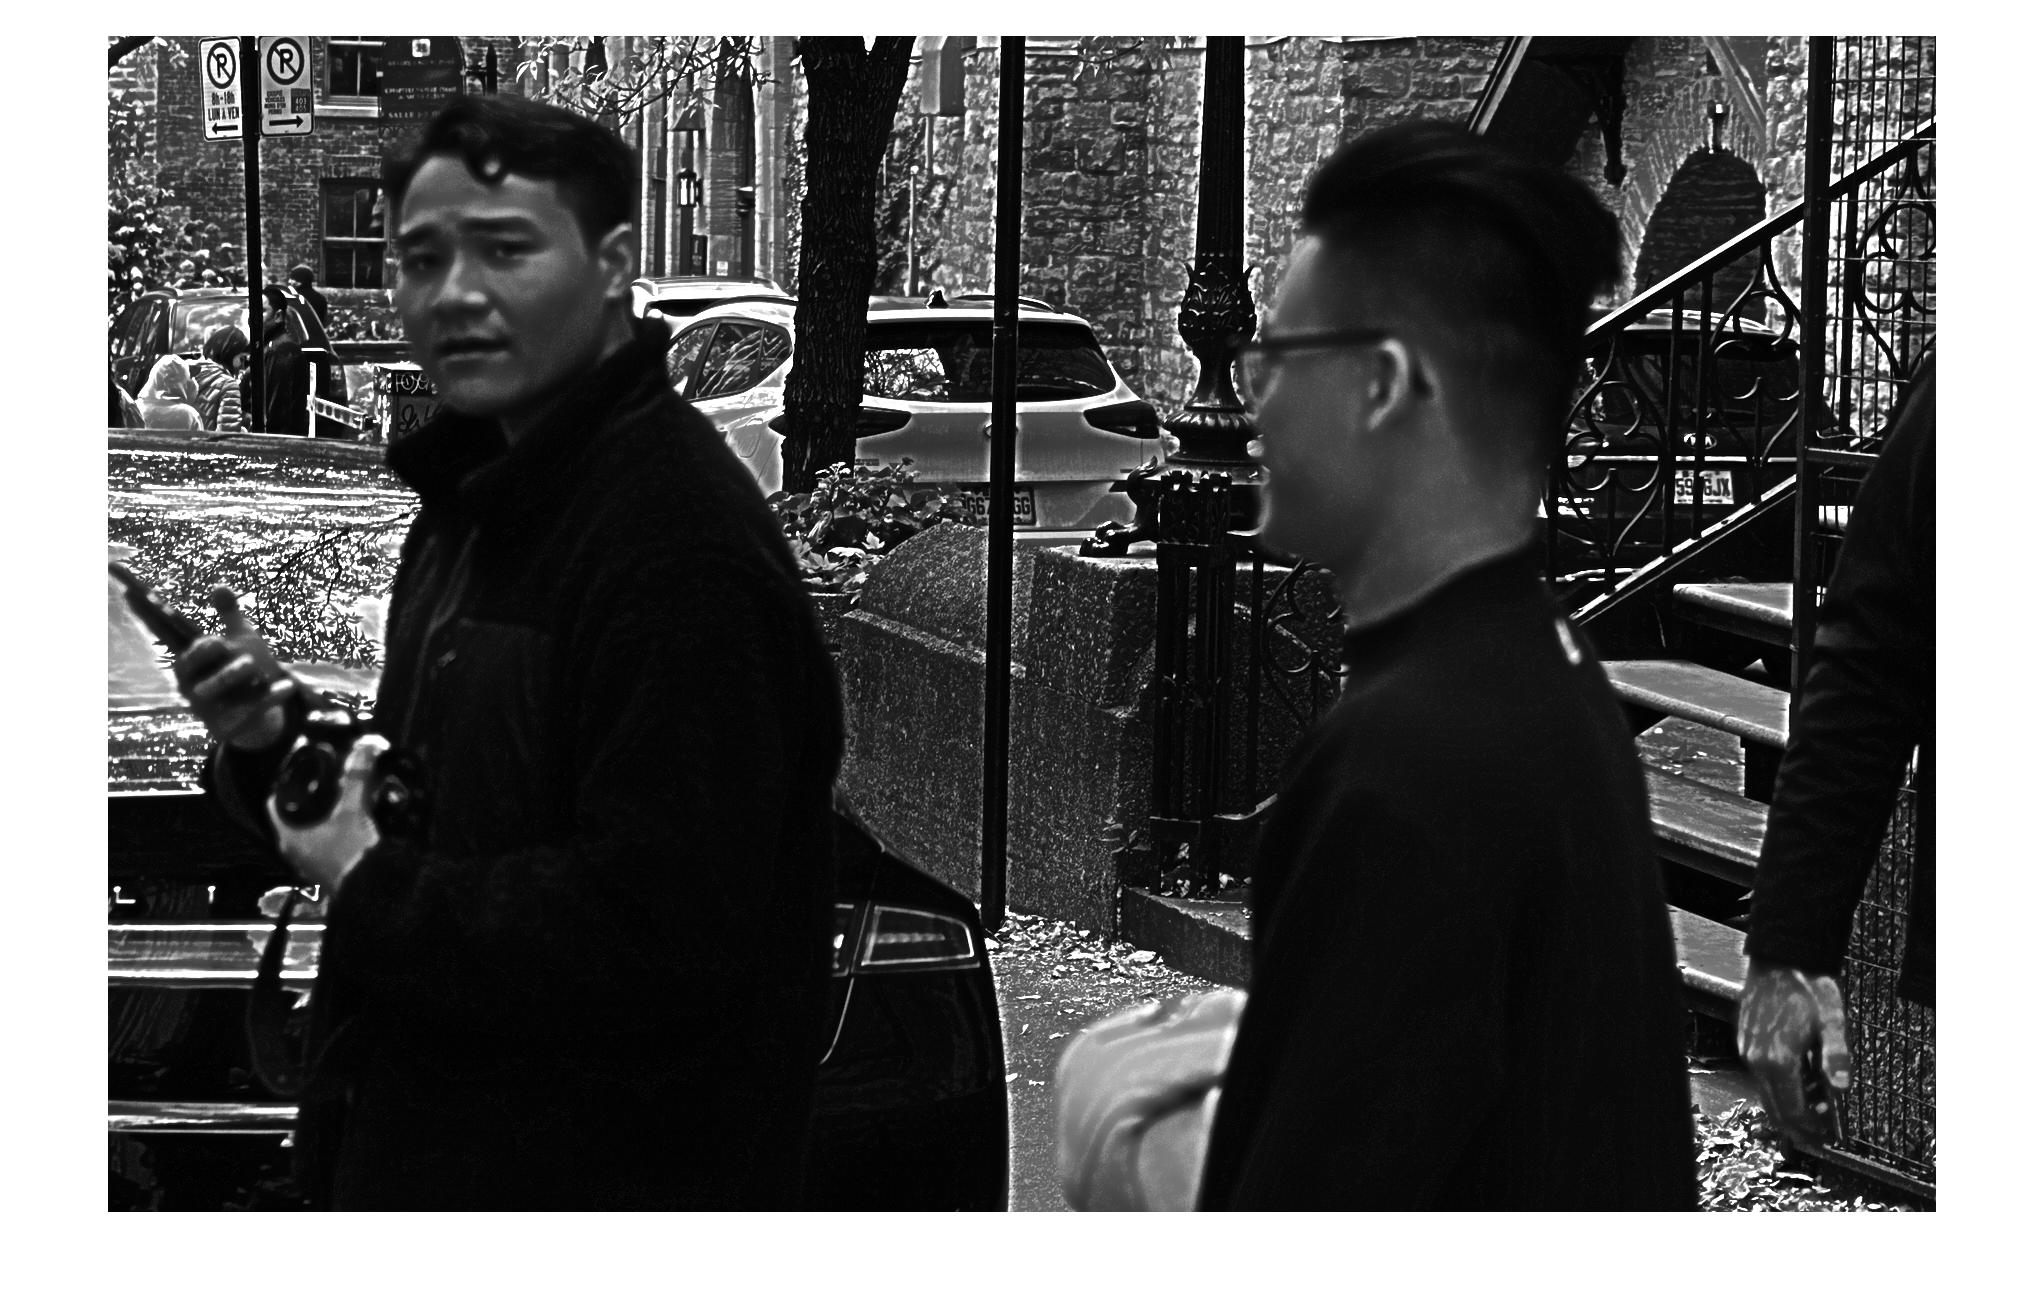
\includegraphics[width=\linewidth]{images/img12.jpg}
\caption{}
\end{subfigure}
\caption{(a) Original image. (b) Grayscale image. (c) Image blurred using Gaussian with lowpass filter with \({\sigma} = 5\). (d) Mask. (e) Result of unsharp masking with \(k = 1\). (f) Result of high-boost filtering with \(k = 5\).}
\label{fig:image sharpening}
\end{figure}

\clearpage
\subsection{Problem 4}

\begin{lstlisting}[language=Matlab]

% Assignment 2
% Part 1
% P4

% Load the original image
img = imread('/lamnguyen/Desktop/School/
Computer-Vision/A2/images/ottawa.jpg');

% Displaying Input Image
img = uint8(img);
figure; 
imshow(img); 

% Convert the image to grayscale
gray_img = rgb2gray(img);
figure; 
imshow(gray_img);

% Add Gaussian noise with 
% mean = 0, variance = 0.01
noise_img1 = imnoise(gray_img, 
                    'gaussian');
figure; 
imshow(noise_img1);

% mean = 0, variance = 0.1
noise_img2 = imnoise(gray_img, 
            'gaussian', 0, 0.1);
figure; 
imshow(noise_img2);

% Remove noise by average filter
% Create average filter
h1 = fspecial('average',[5 5]);
h2 = fspecial('average',[7 7]);

% Apply filter to the image
af_img1 = imfilter(noise_img1, h1);
figure; 
imshow(af_img1);

af_img2 = imfilter(noise_img2, h2);
figure; 
imshow(af_img2);

% Remove noise by Gausian filter
gauss_img1 = imgaussfilt(noise_img1, 1);
figure; 
imshow(gauss_img1);

gauss_img2 = imgaussfilt(noise_img2, 5);
figure; 
imshow(gauss_img2);

\end{lstlisting}

\begin{figure}[h!]
\centering
\begin{subfigure}[b]{0.4\linewidth}
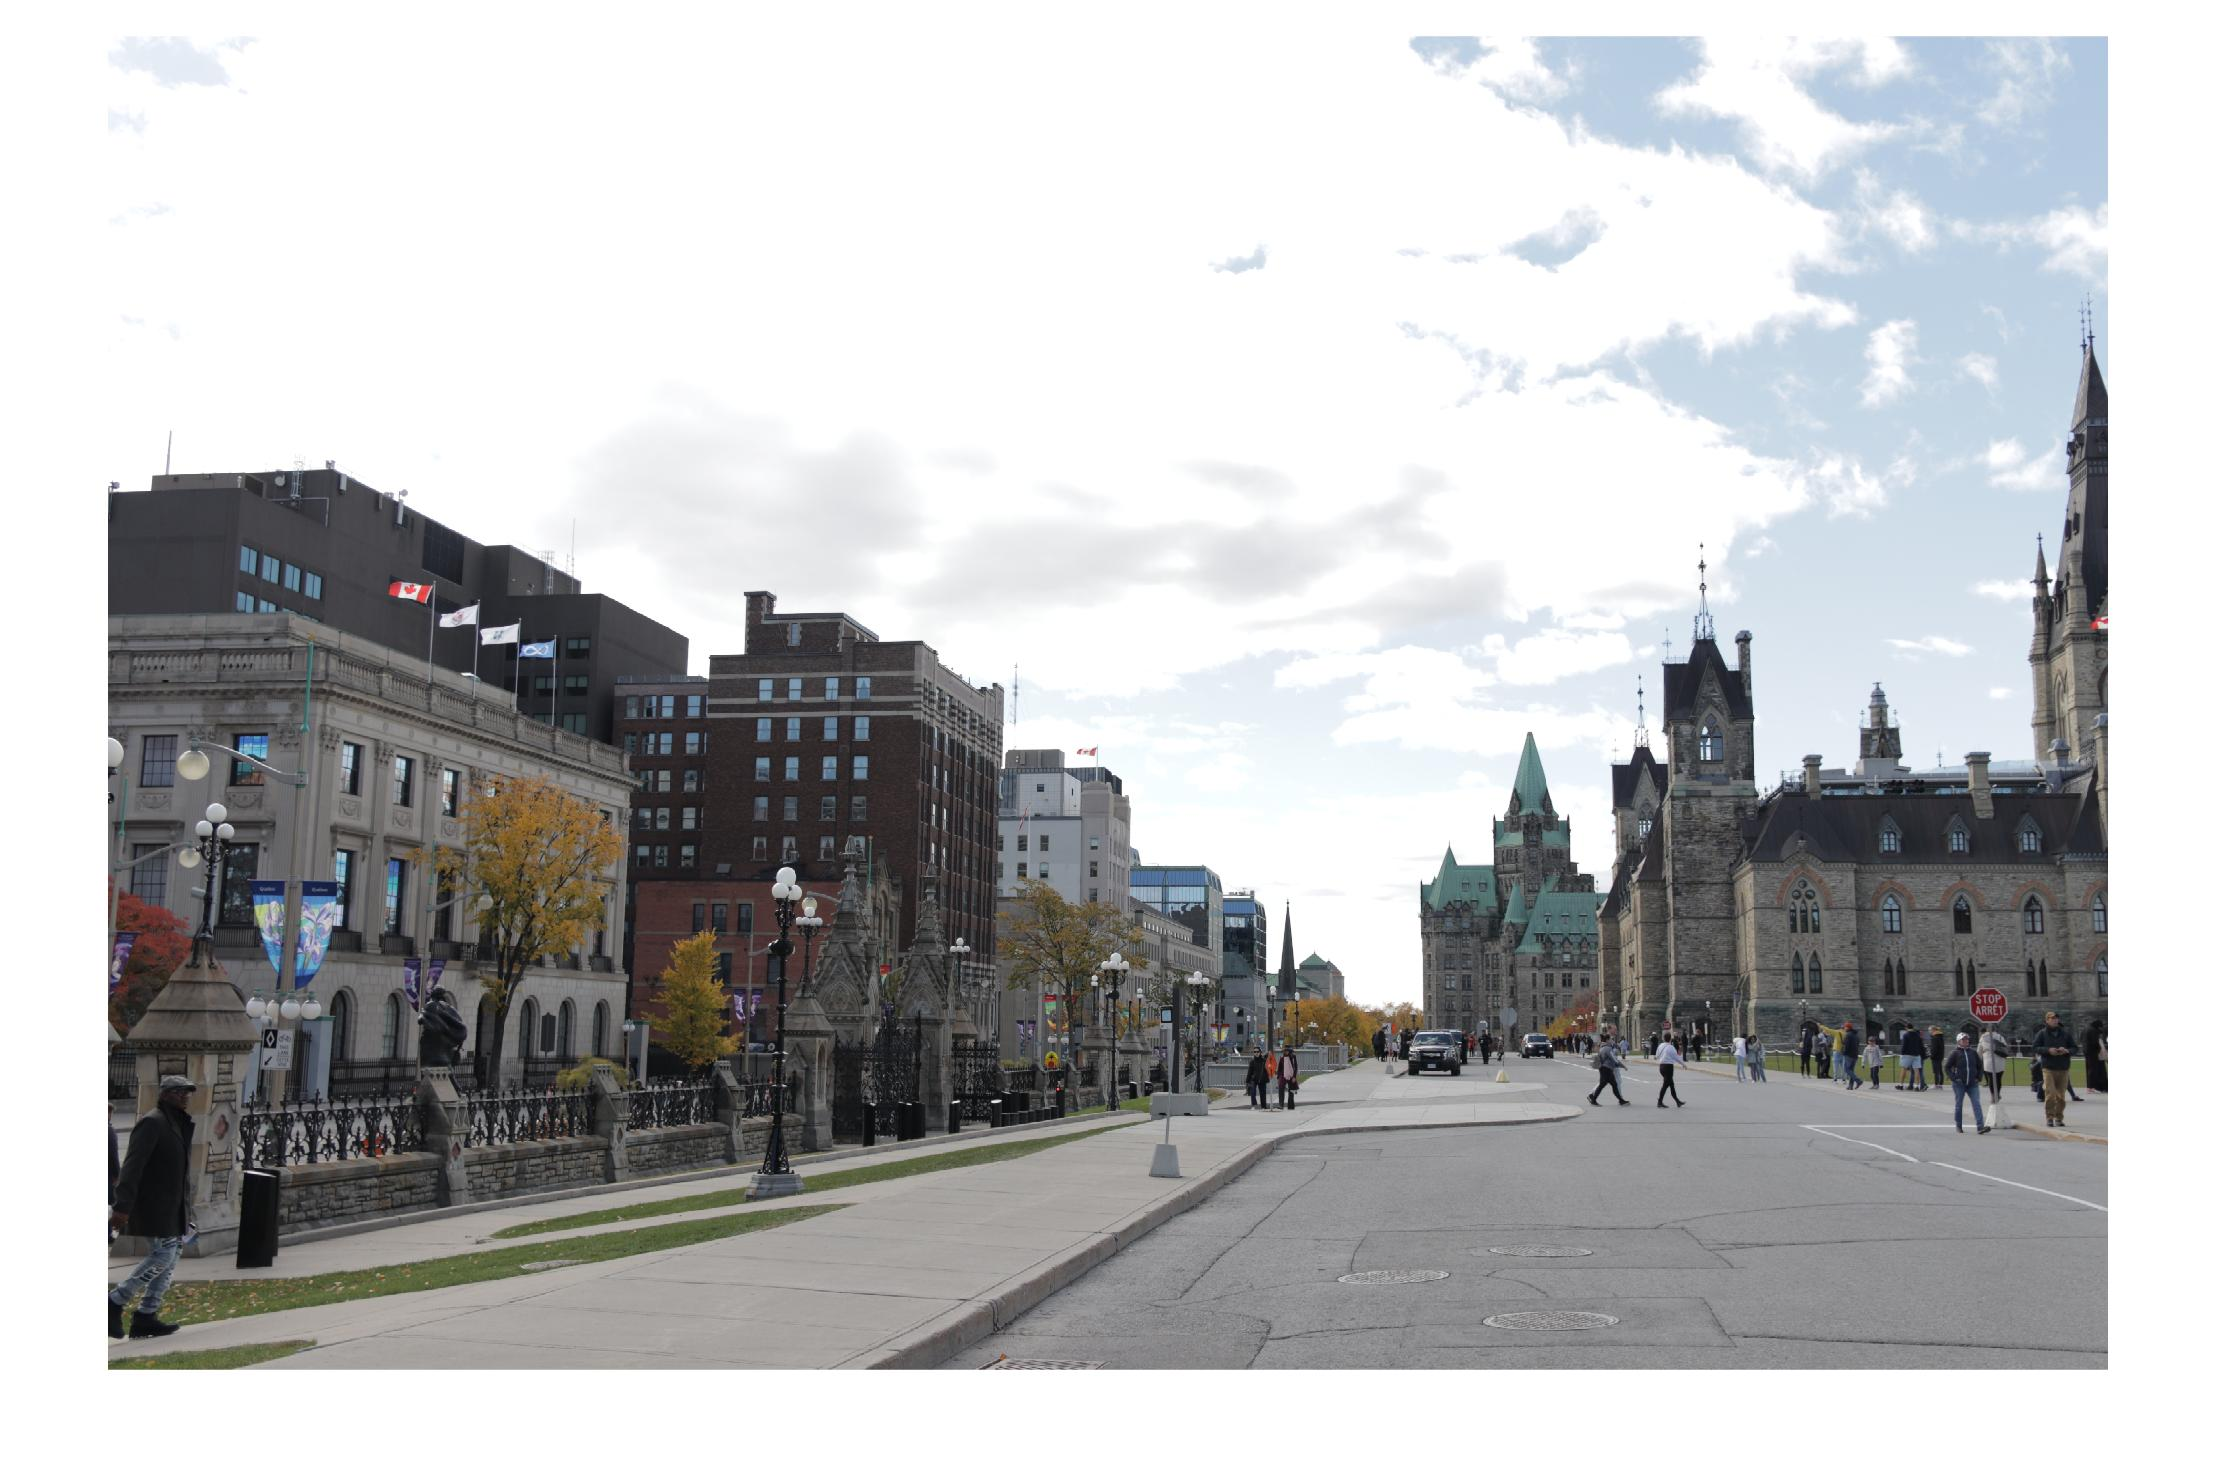
\includegraphics[width=\linewidth]{images/img13.jpg}
\caption{Original image}
\end{subfigure}
\begin{subfigure}[b]{0.4\linewidth}
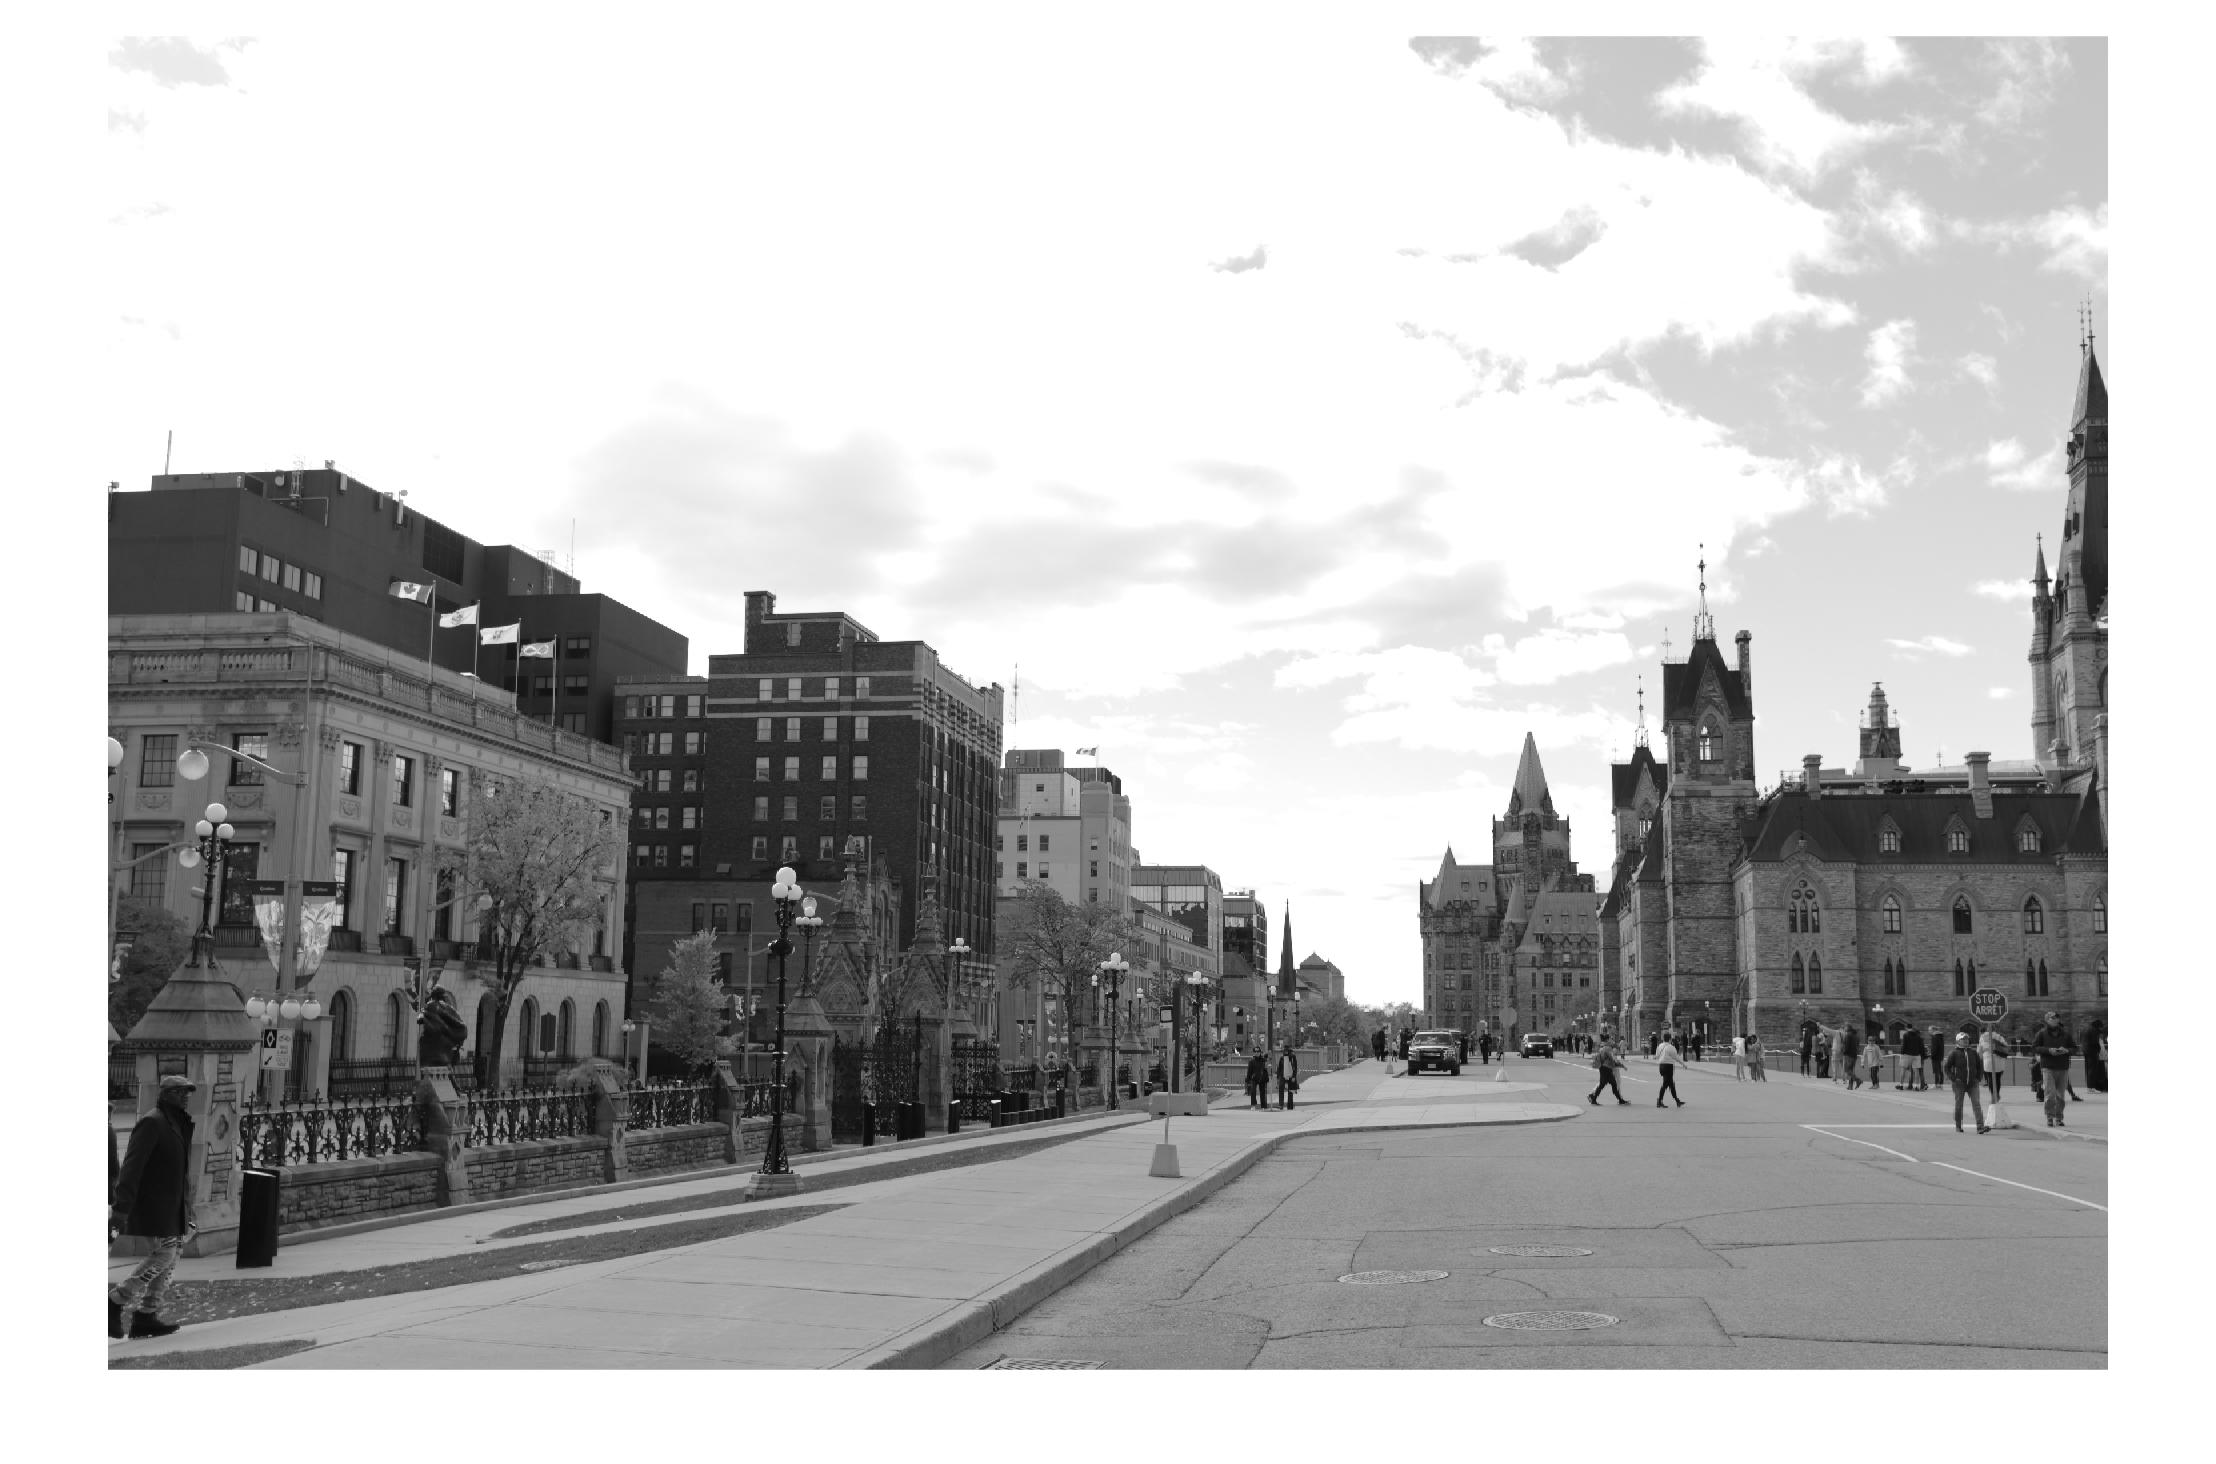
\includegraphics[width=\linewidth]{images/img14.jpg}
\caption{Grayscale image}
\end{subfigure}
\begin{subfigure}[b]{0.4\linewidth}
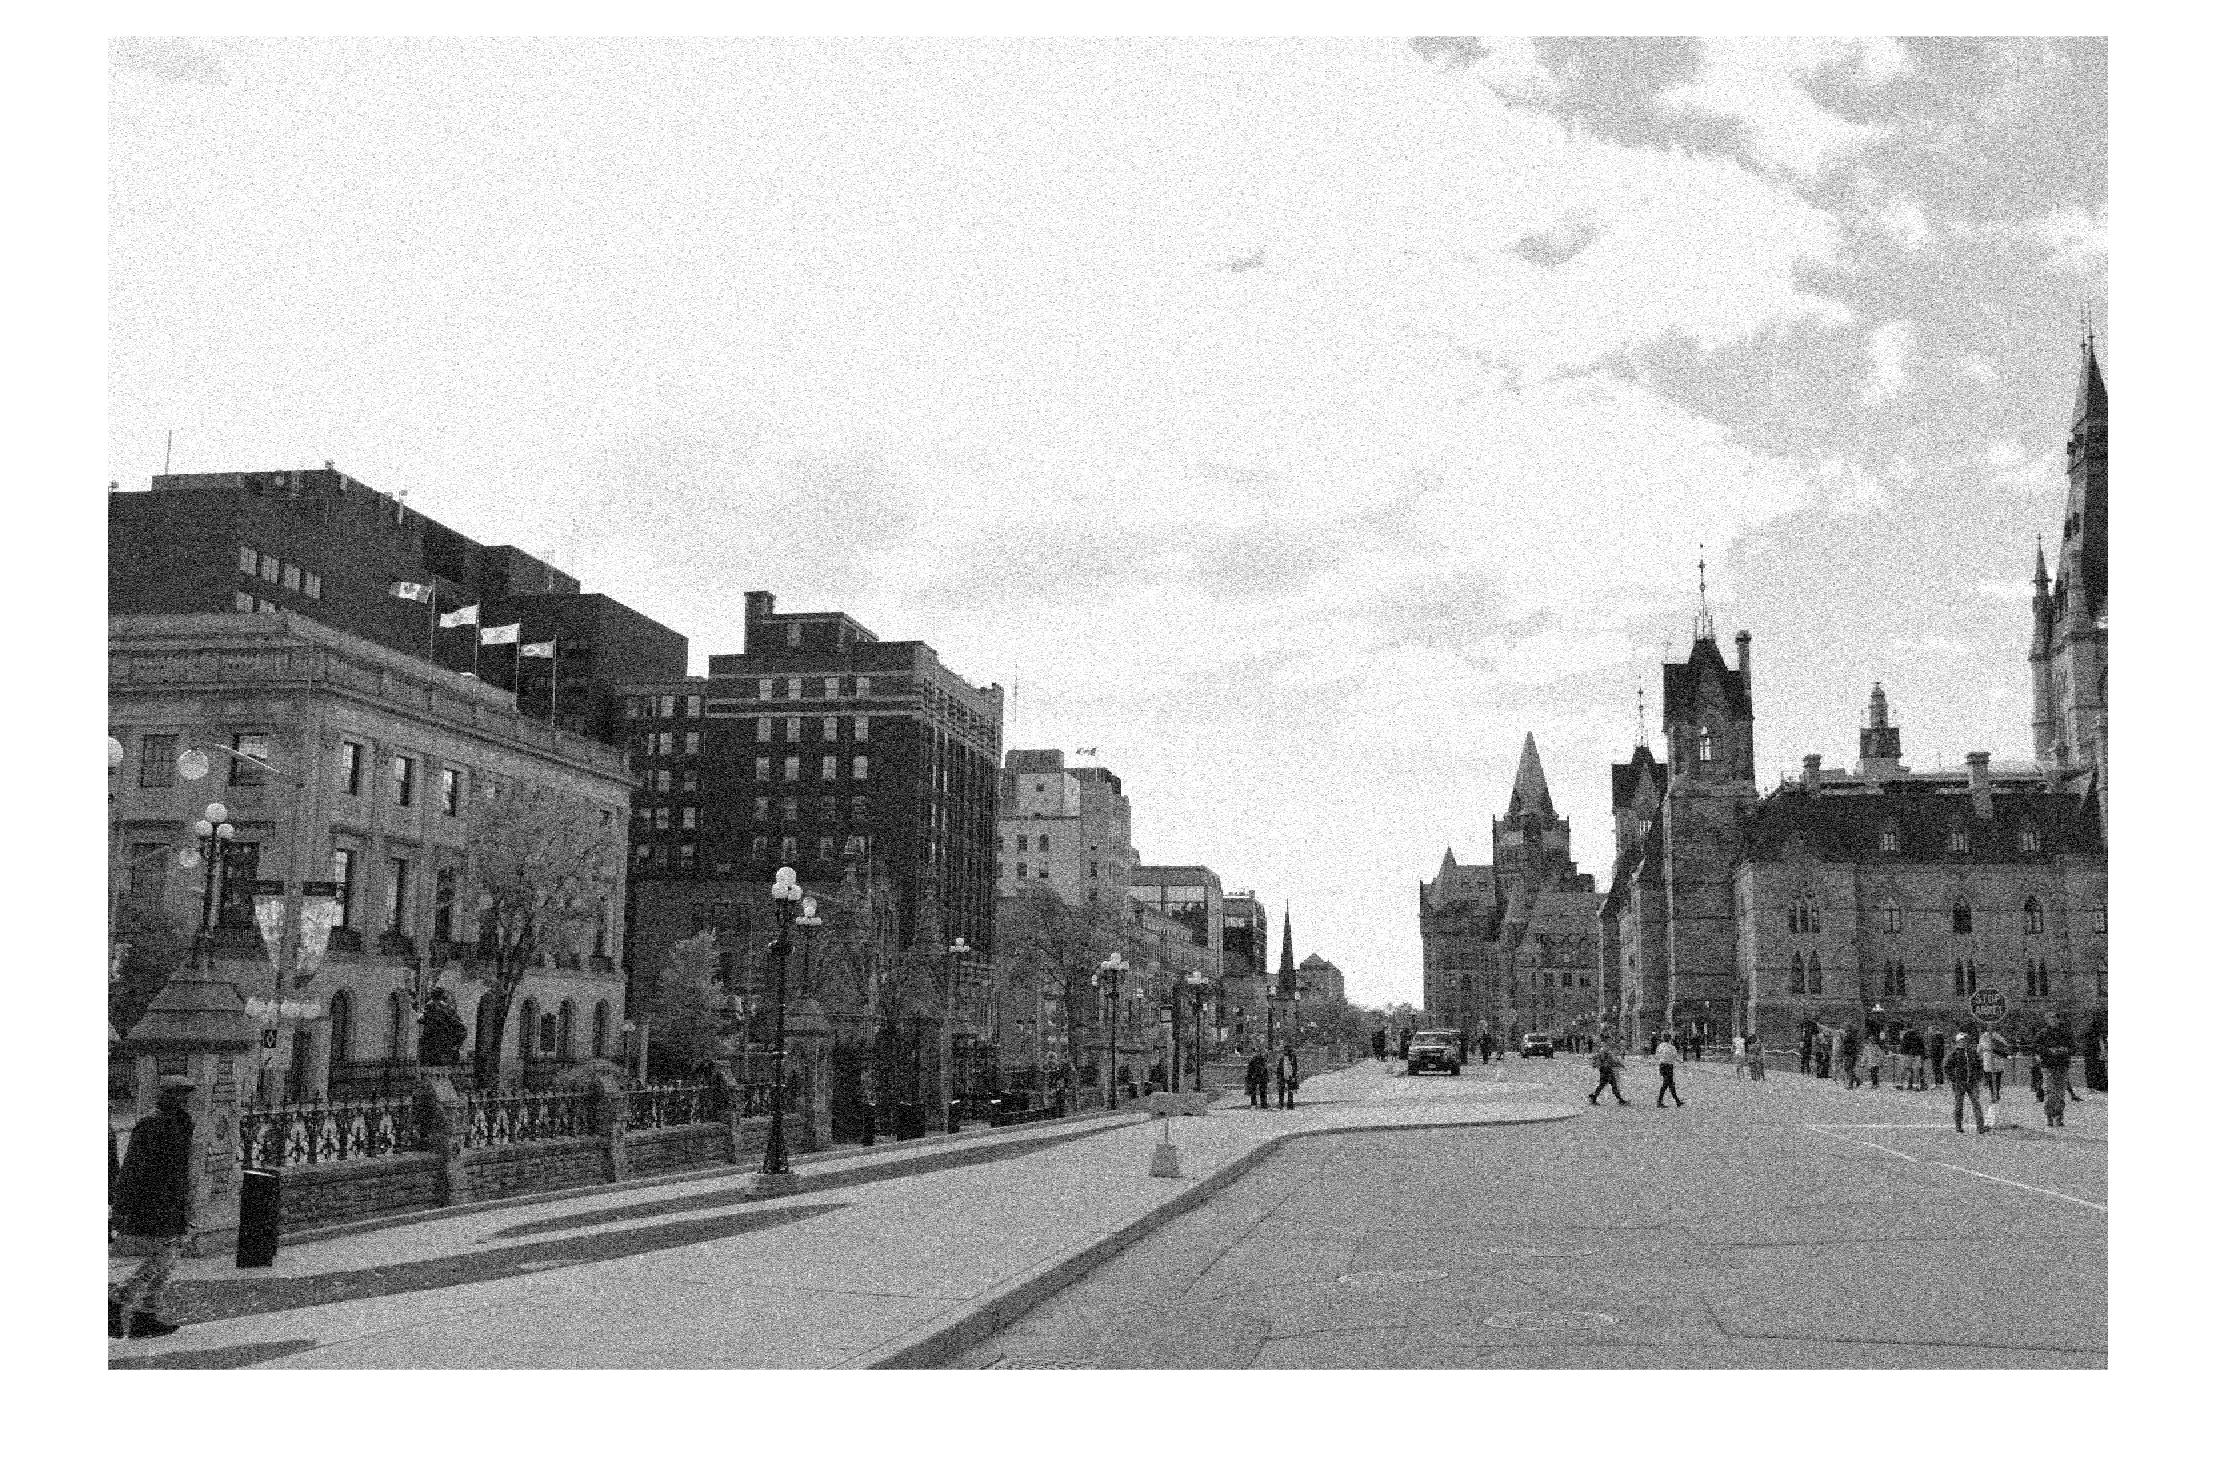
\includegraphics[width=\linewidth]{images/img15.jpg}
\caption{Variance of 0.01}
\end{subfigure}
\begin{subfigure}[b]{0.4\linewidth}
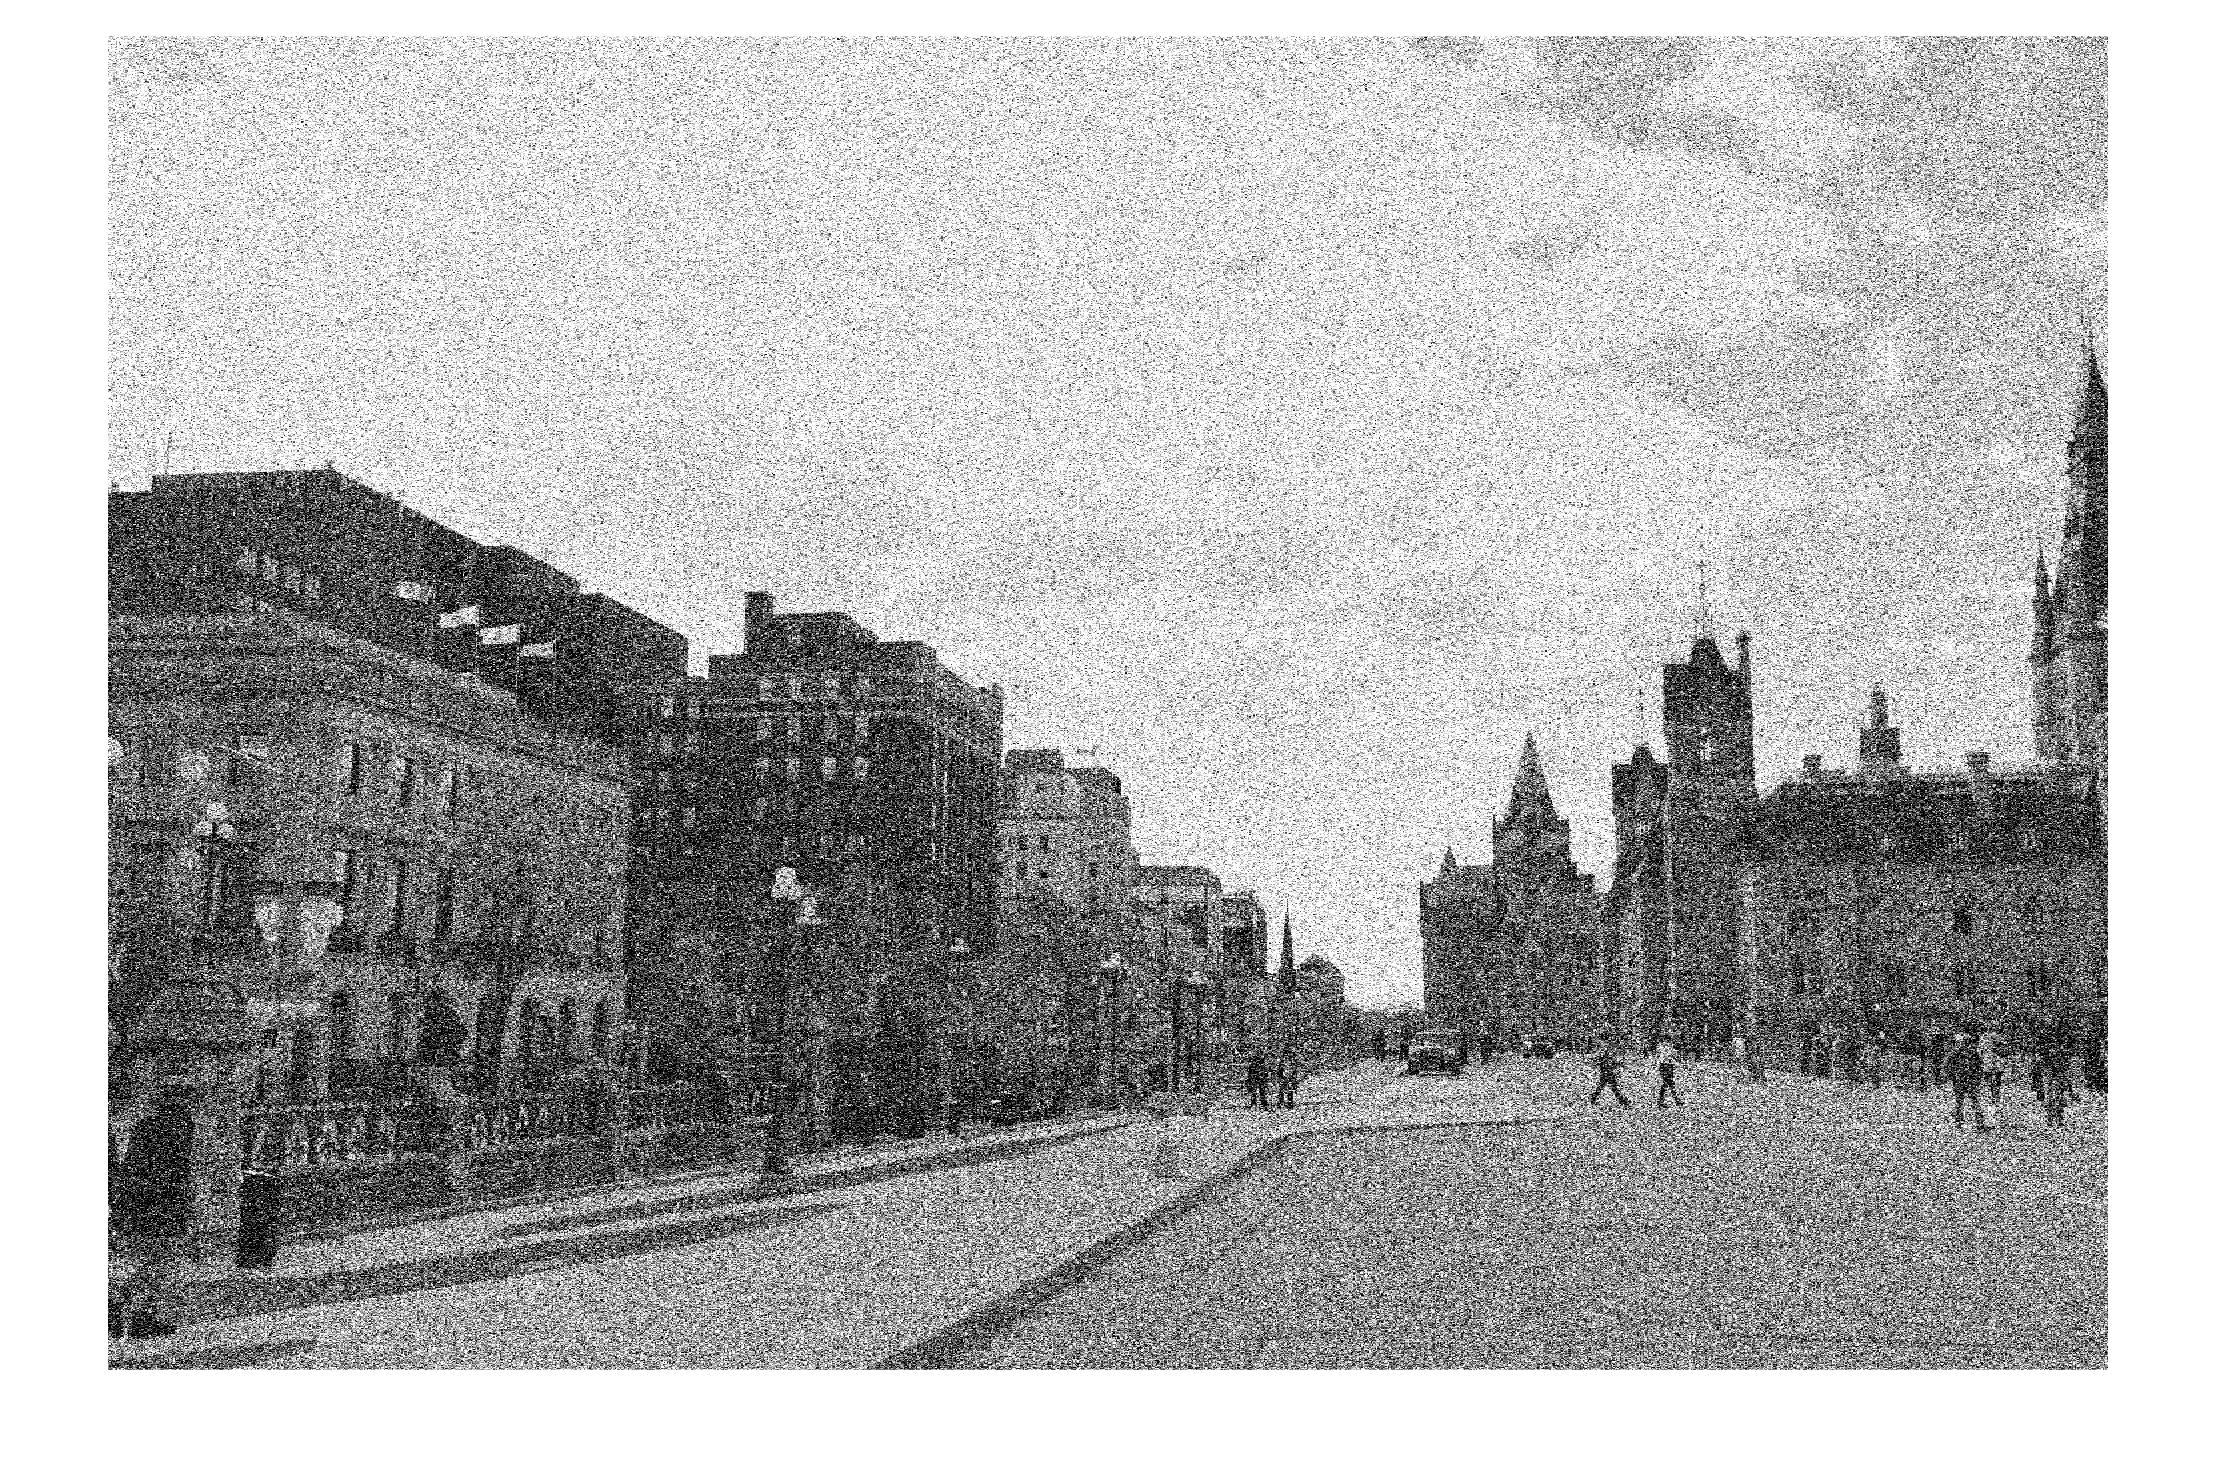
\includegraphics[width=\linewidth]{images/img16.jpg}
\caption{Variance of 0.1}
\end{subfigure}
\caption{Adding Gaussian noise to the image}
\label{fig:Gaussian noise}
\end{figure}

The Gaussian noise was added to the grayscale image with two different noise levels. With the variance of 0.01, less noise was added to the image. On the other hand, more noise produced in the image with the variance of 0.1.

\begin{figure}[h!]
\centering
\begin{subfigure}[b]{0.3\linewidth}
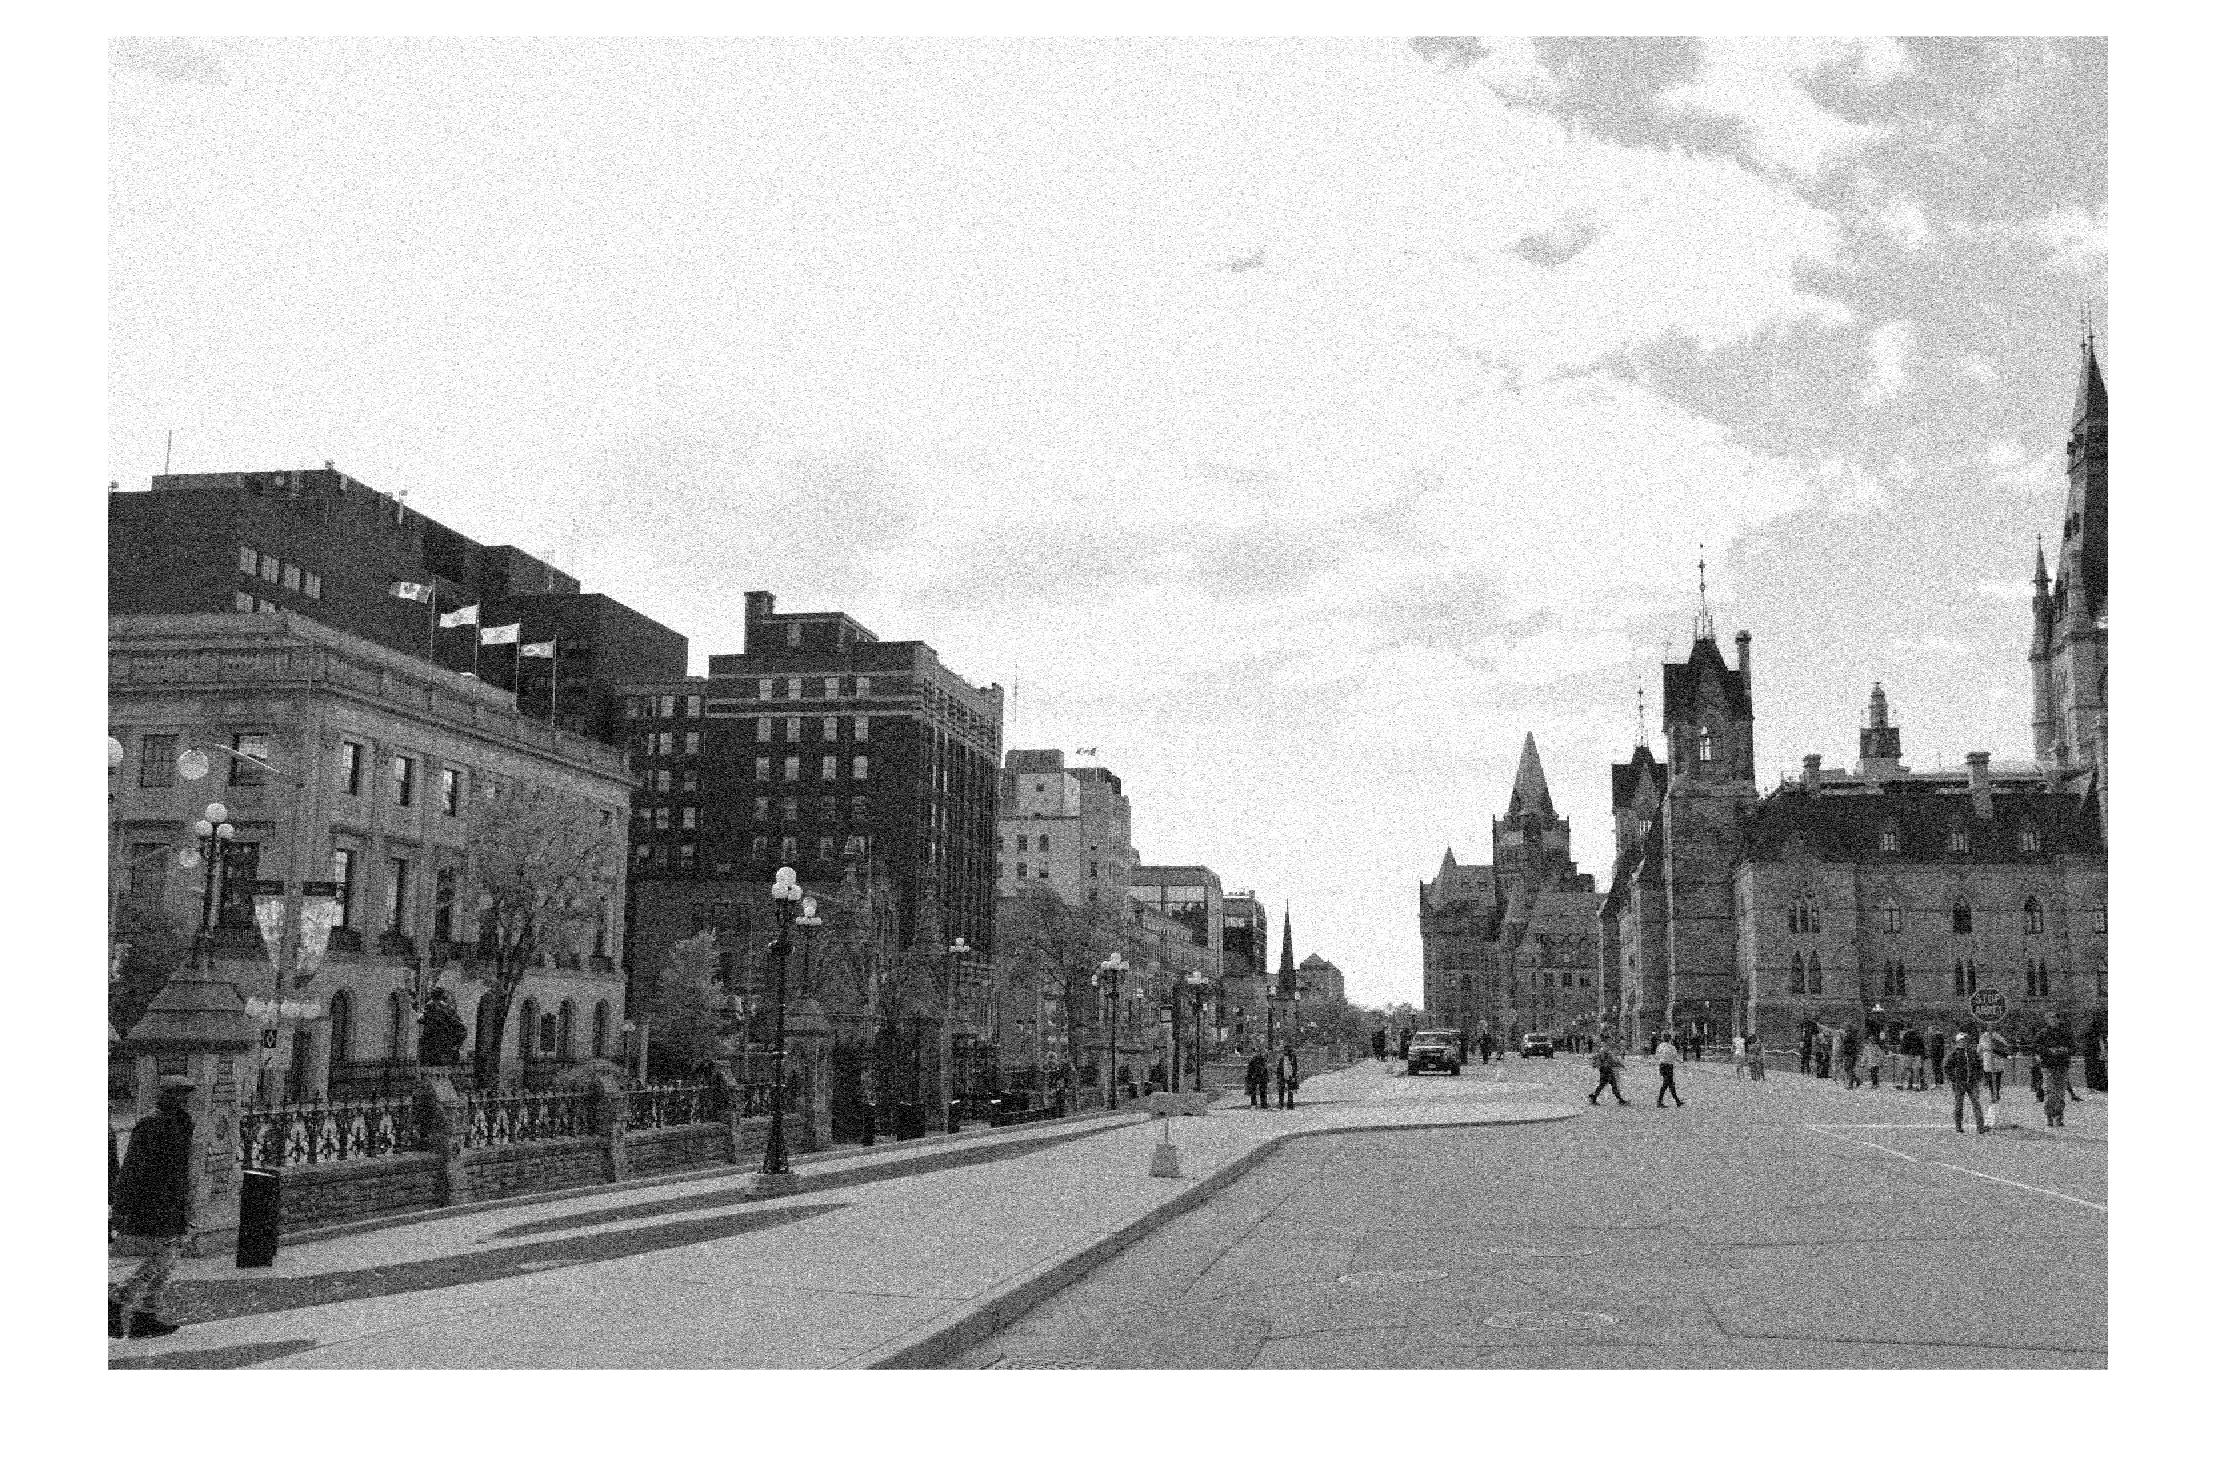
\includegraphics[width=\linewidth]{images/img15.jpg}
\caption{Noise image}
\end{subfigure}
\begin{subfigure}[b]{0.3\linewidth}
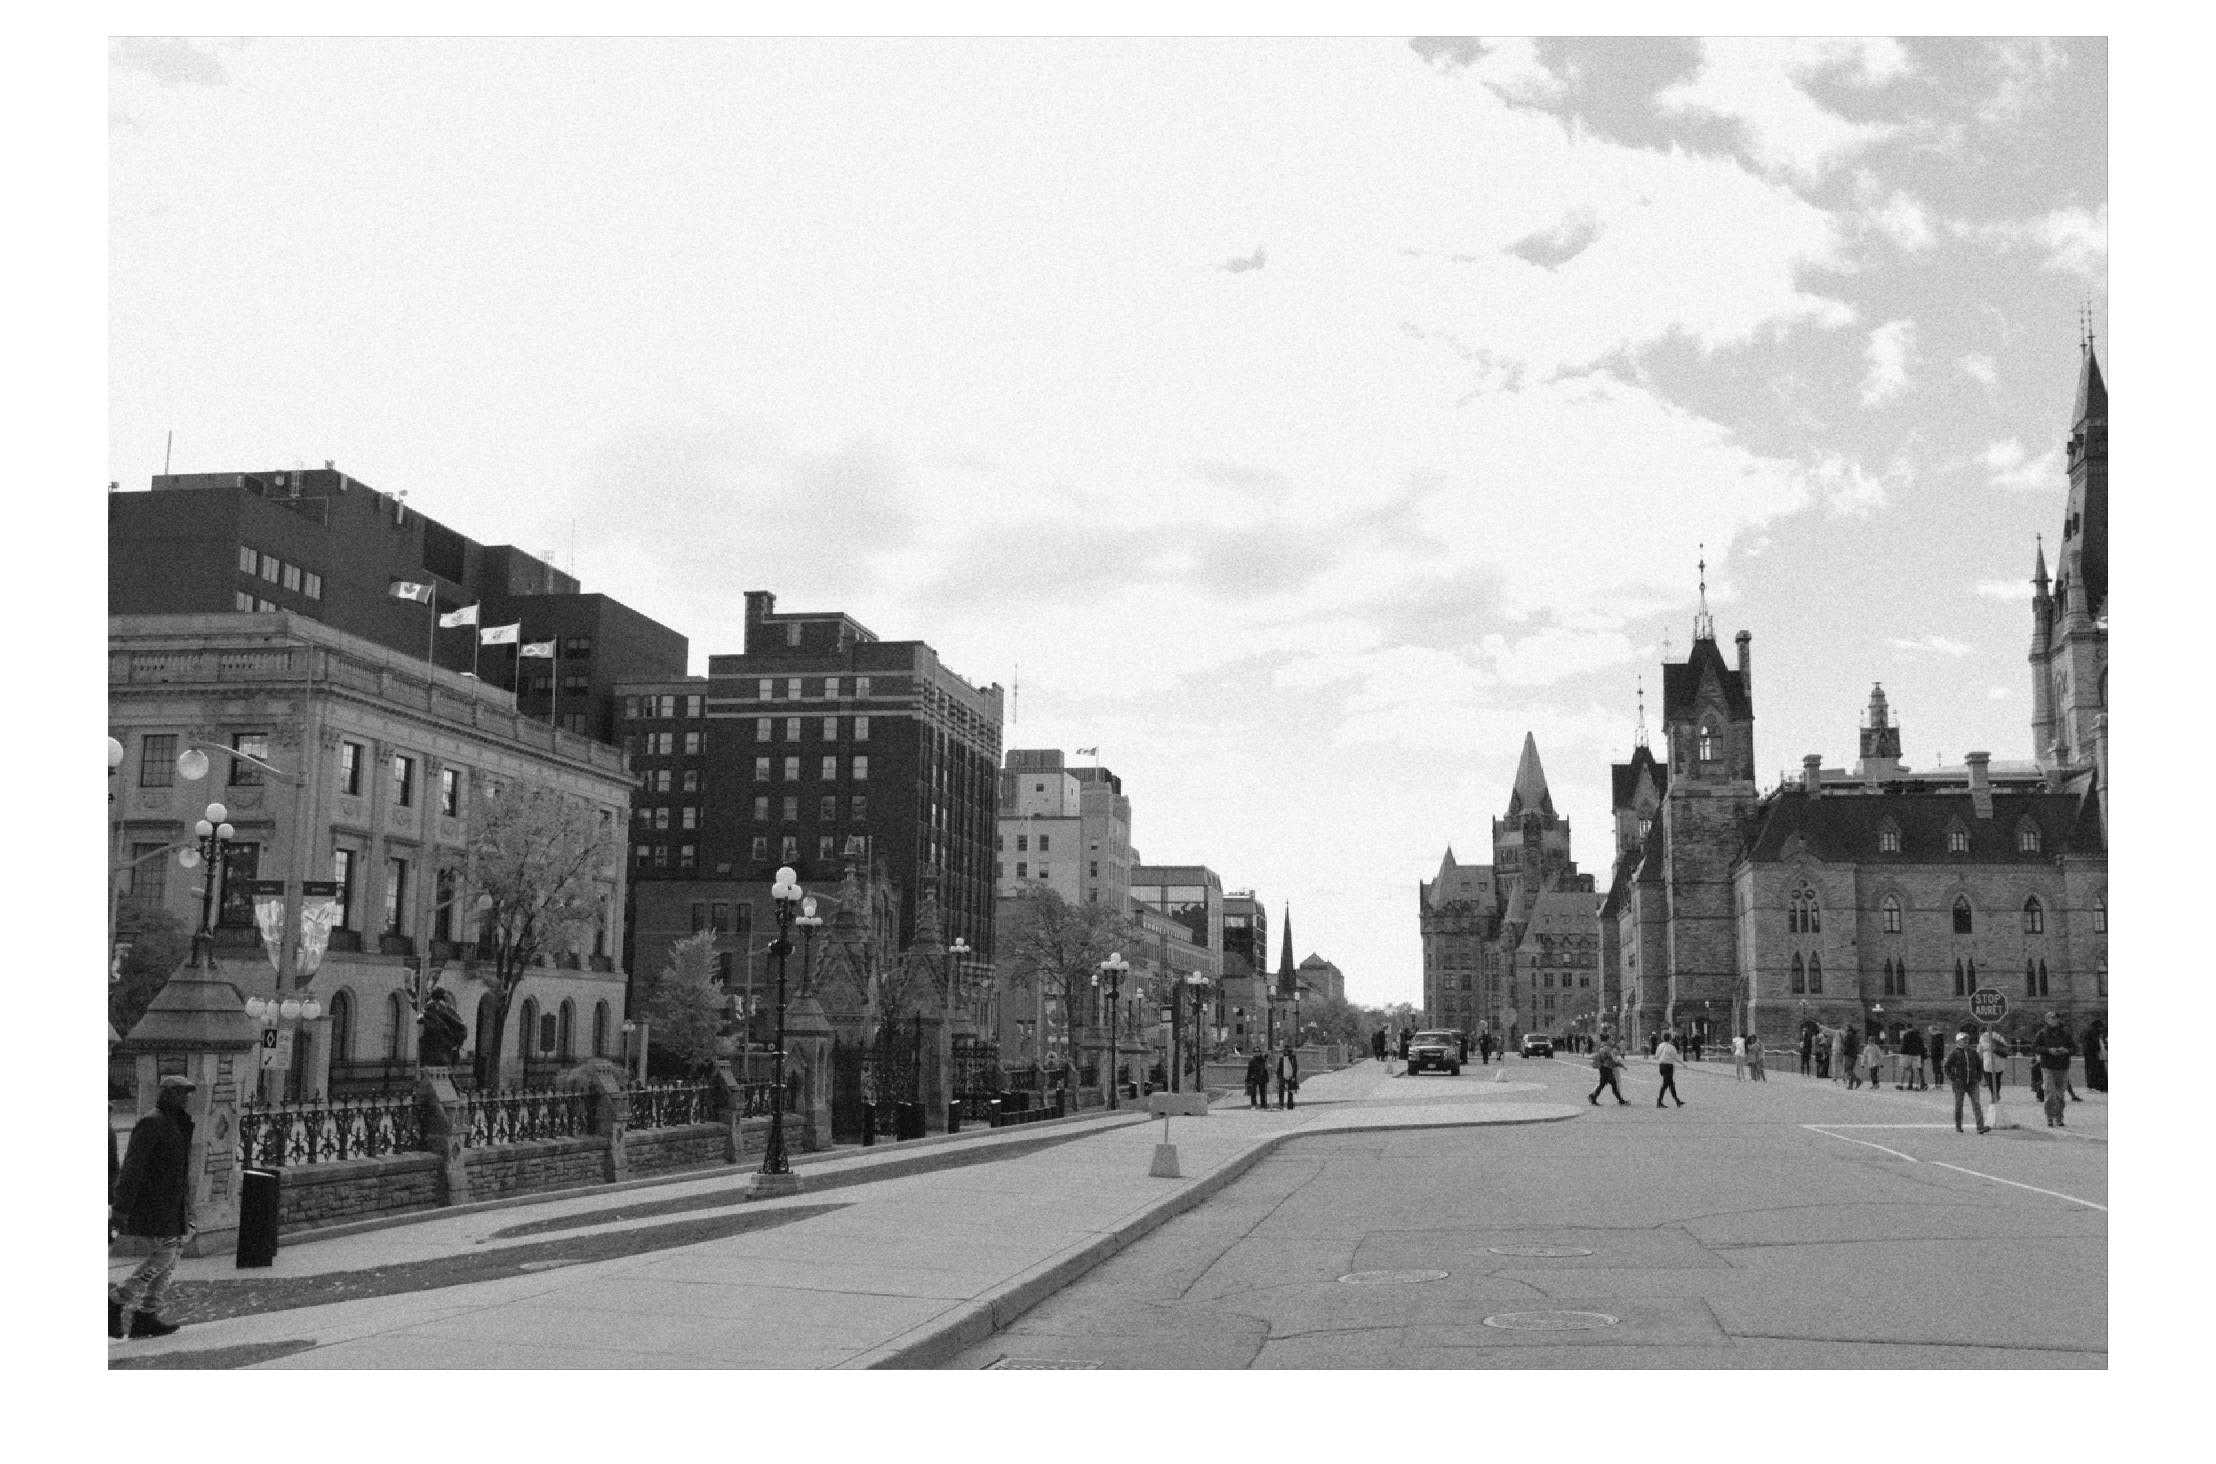
\includegraphics[width=\linewidth]{images/img17.jpg}
\caption{Average filter}
\end{subfigure}
\begin{subfigure}[b]{0.3\linewidth}
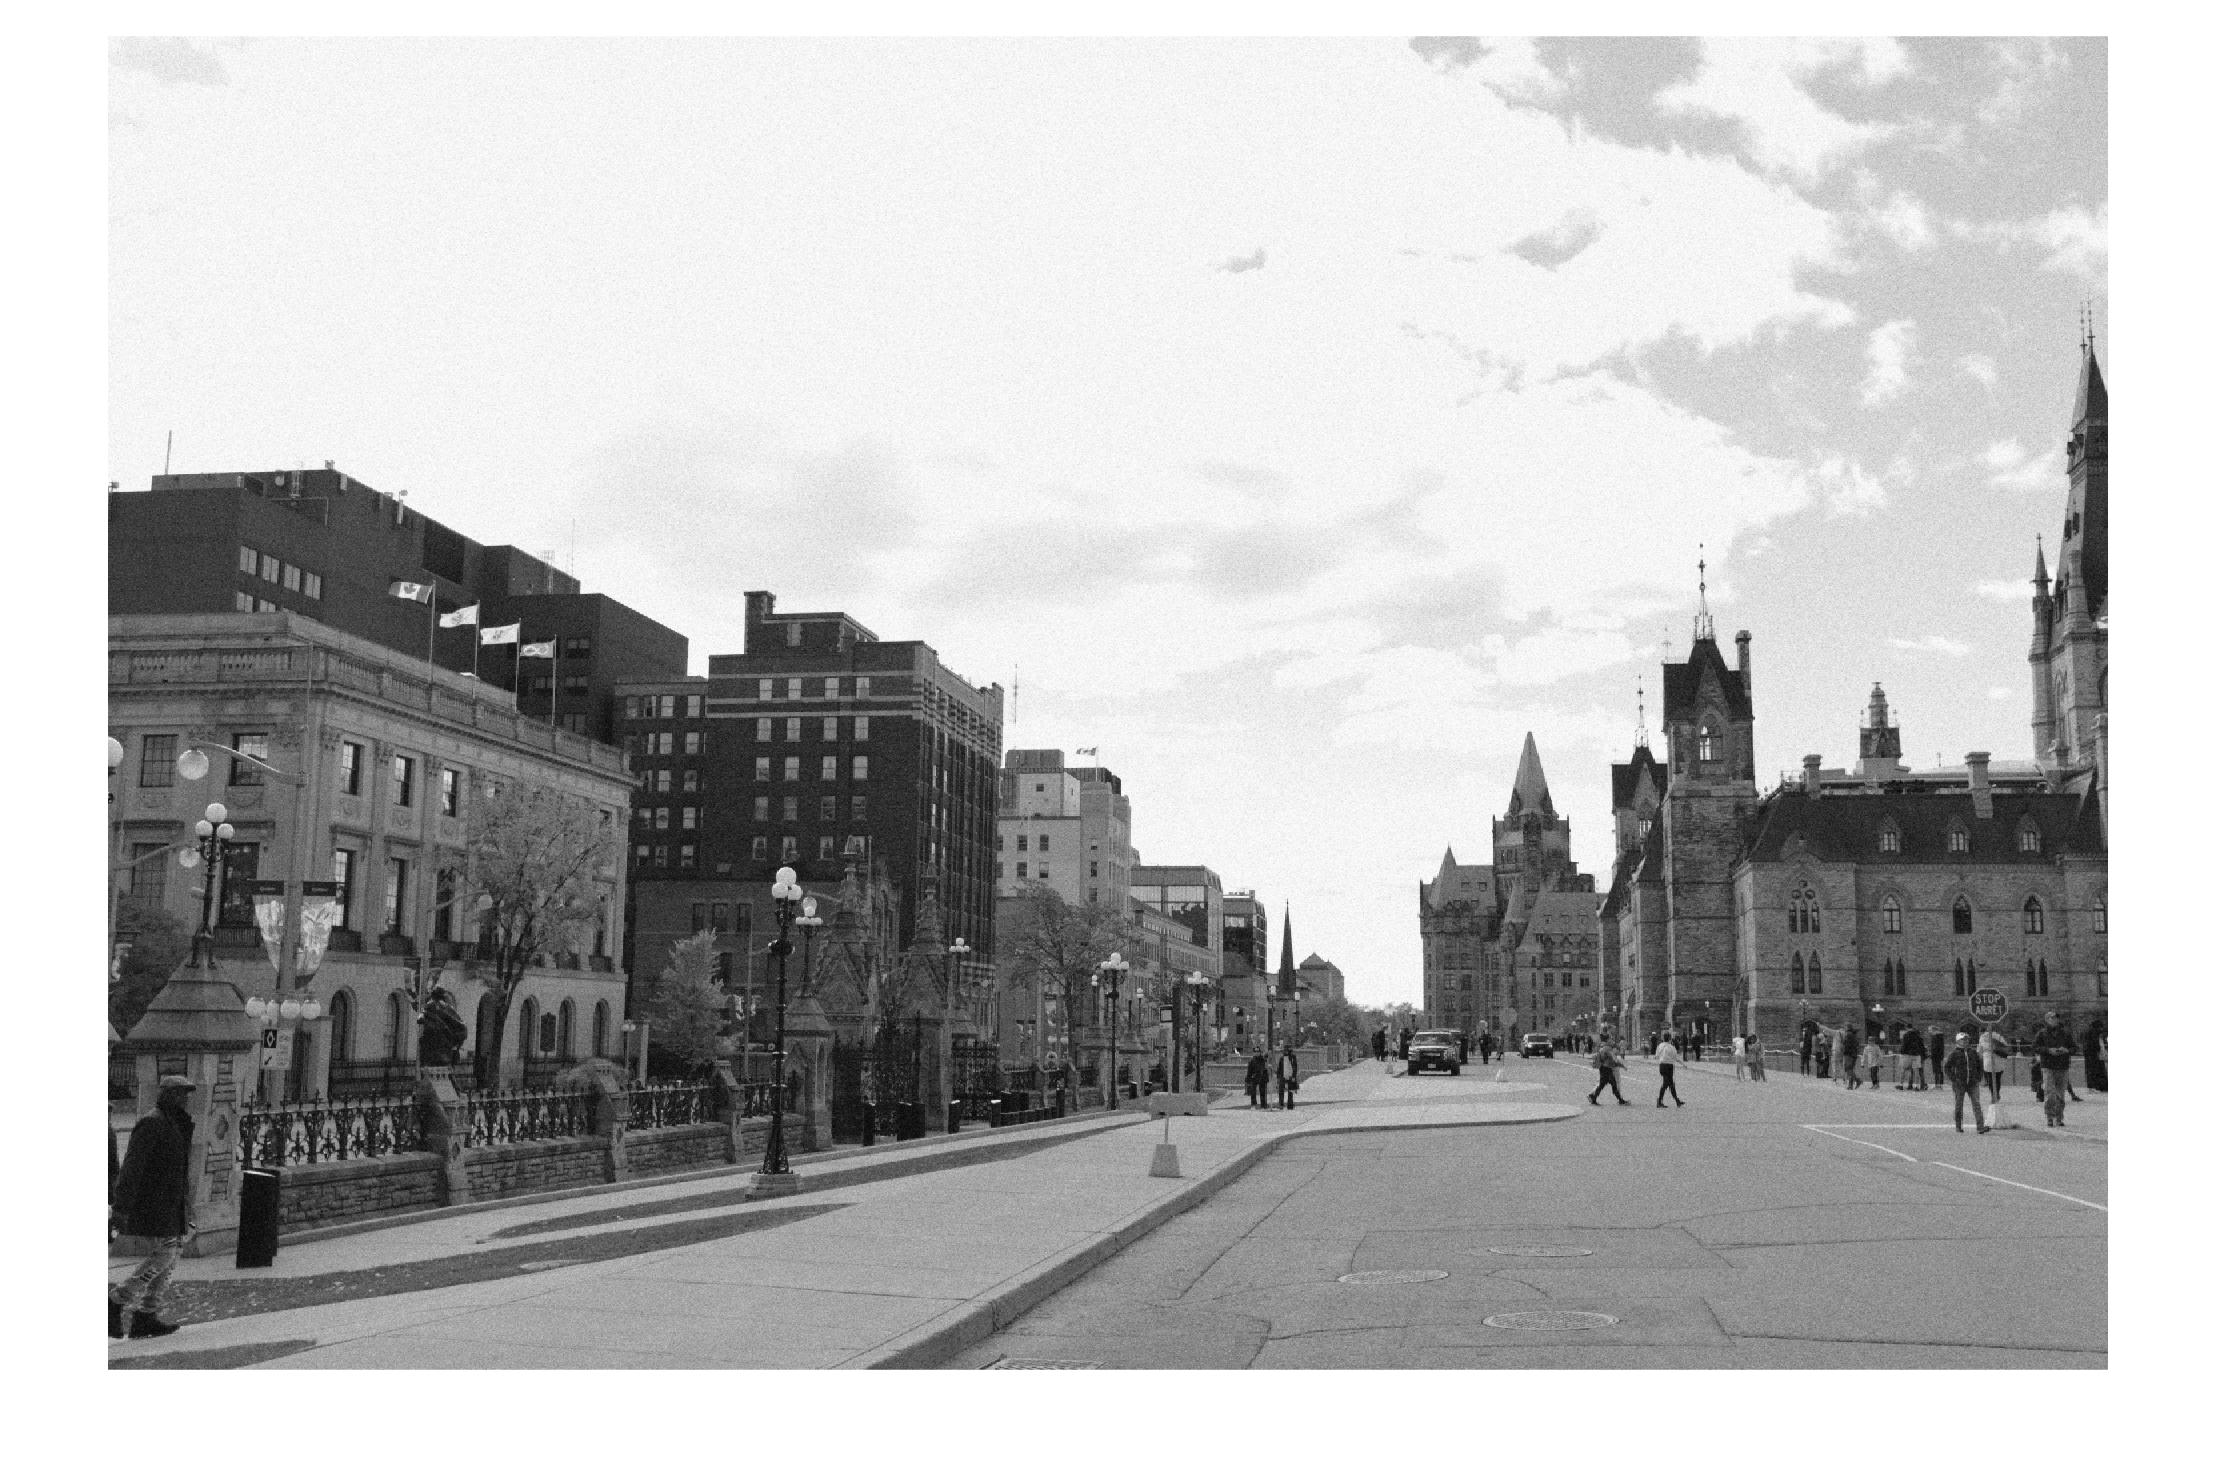
\includegraphics[width=\linewidth]{images/img19.jpg}
\caption{Gaussian filter}
\end{subfigure}
\caption{Applying filters to the image with less noise}
\label{fig:less noise image}
\end{figure}

For the image with less noise, a 5x5 average filter and a Gaussian filter with standard deviation of 1 were used to remove the noise in the image. Both of the filters worked well since the noise was significantly reduced. 

\begin{figure}[h!]
\centering
\begin{subfigure}[b]{0.3\linewidth}
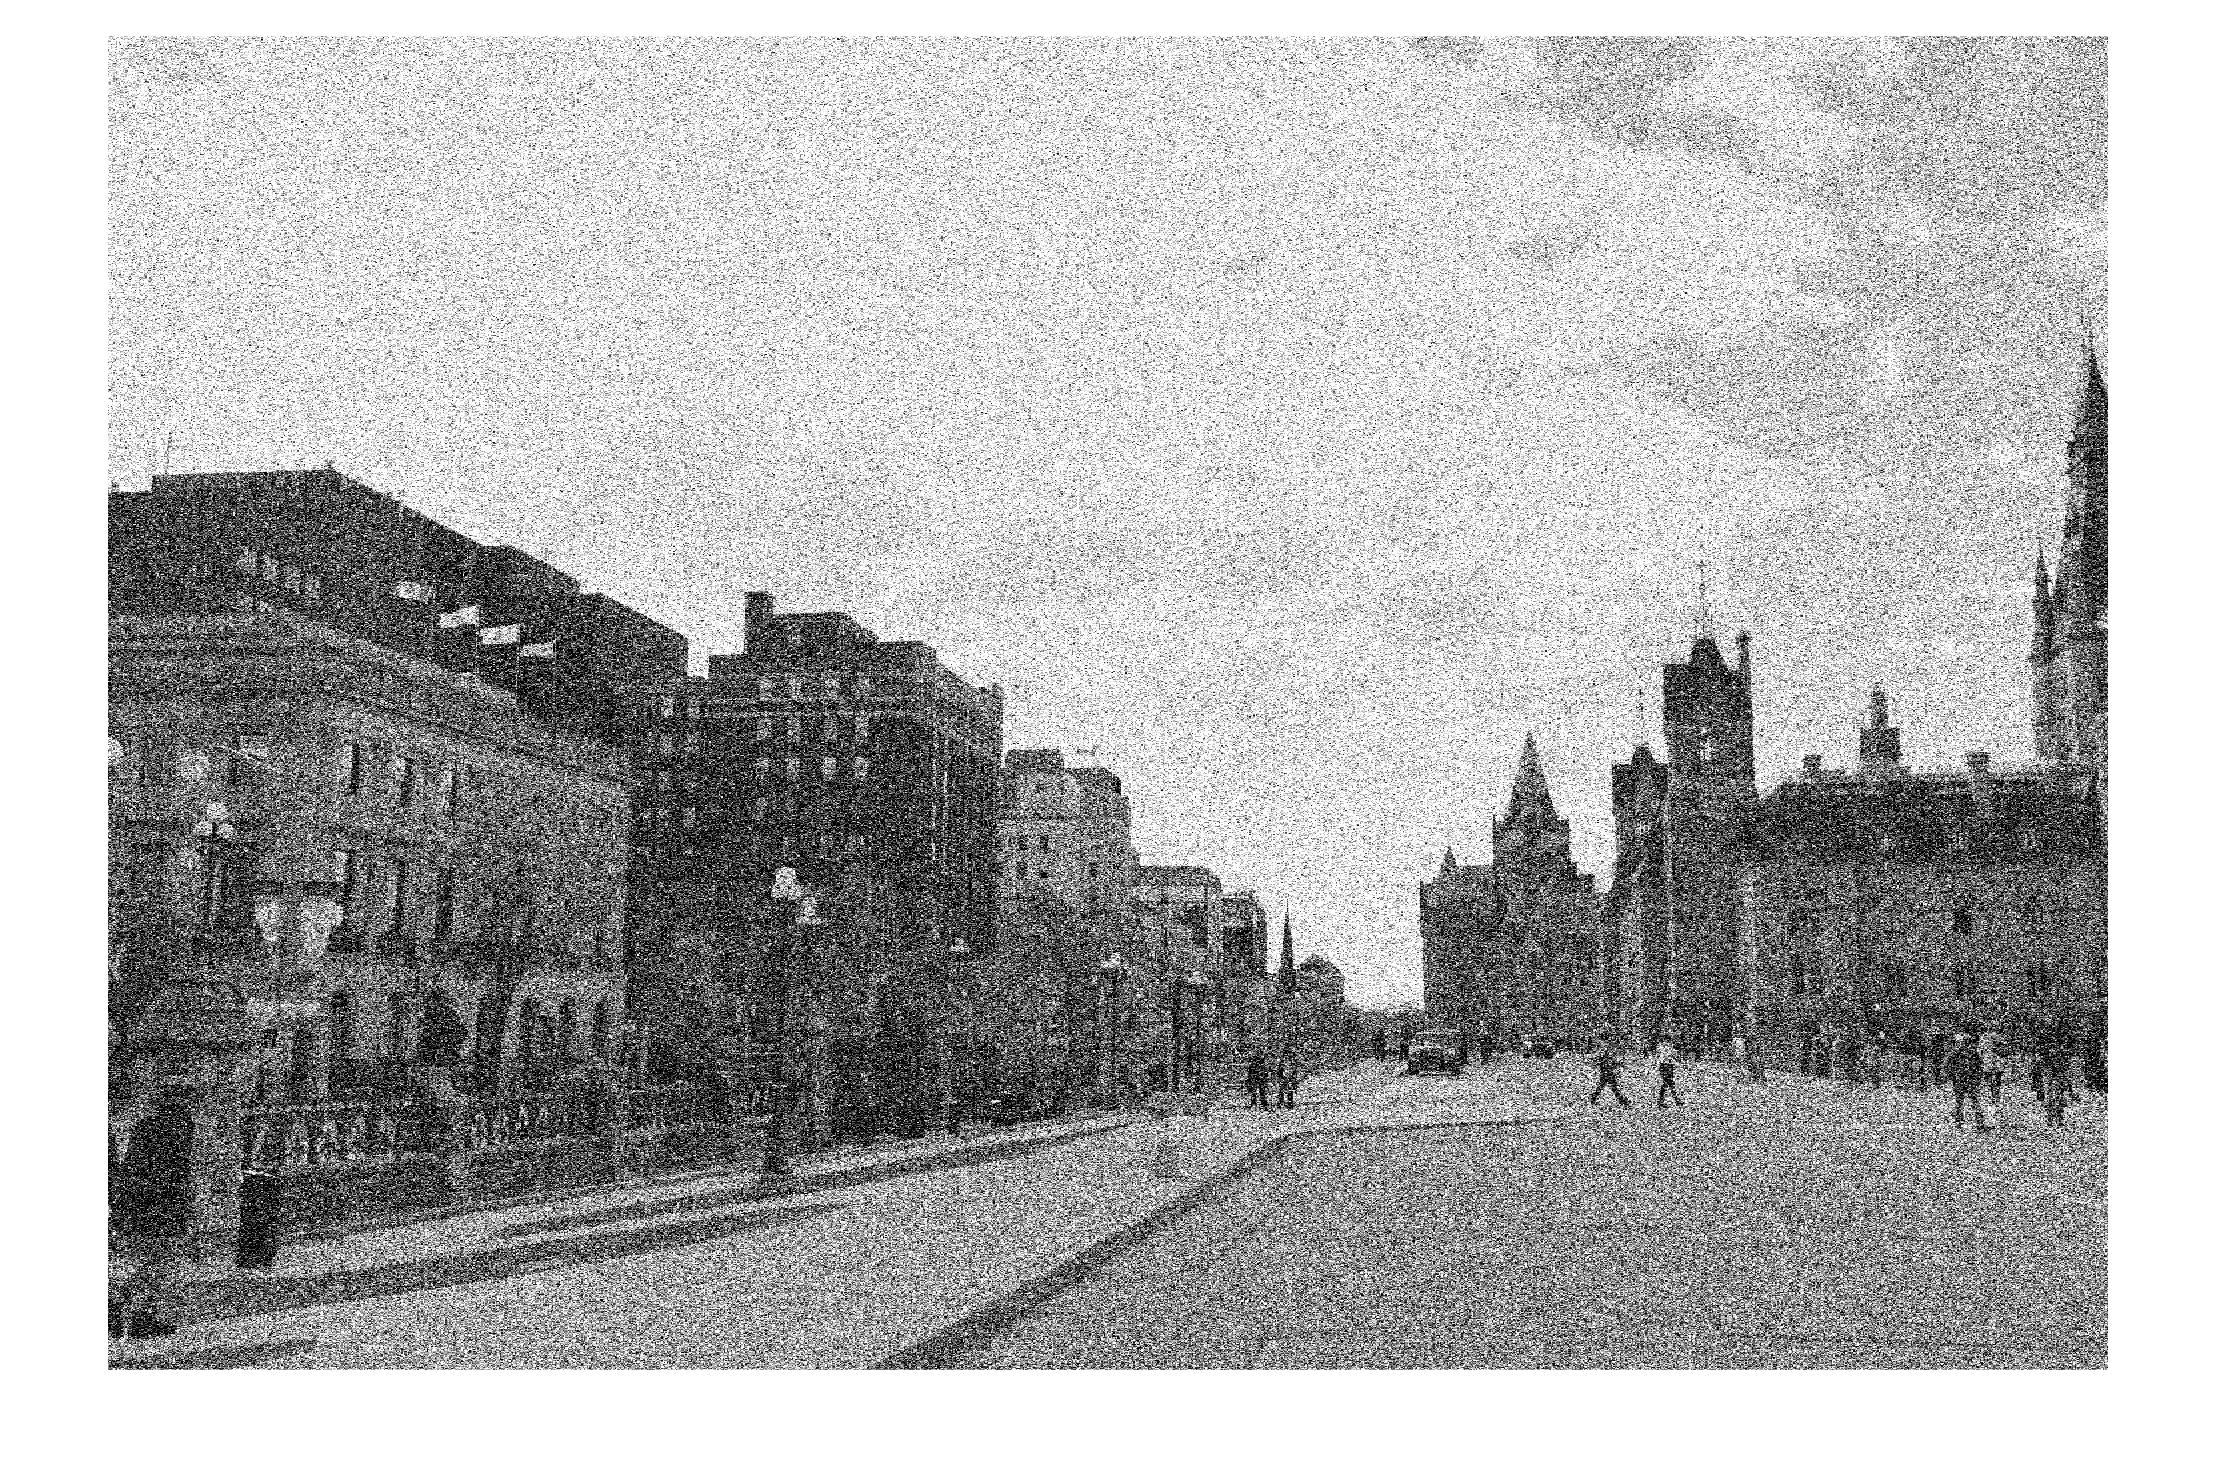
\includegraphics[width=\linewidth]{images/img16.jpg}
\caption{Noise image}
\end{subfigure}
\begin{subfigure}[b]{0.3\linewidth}
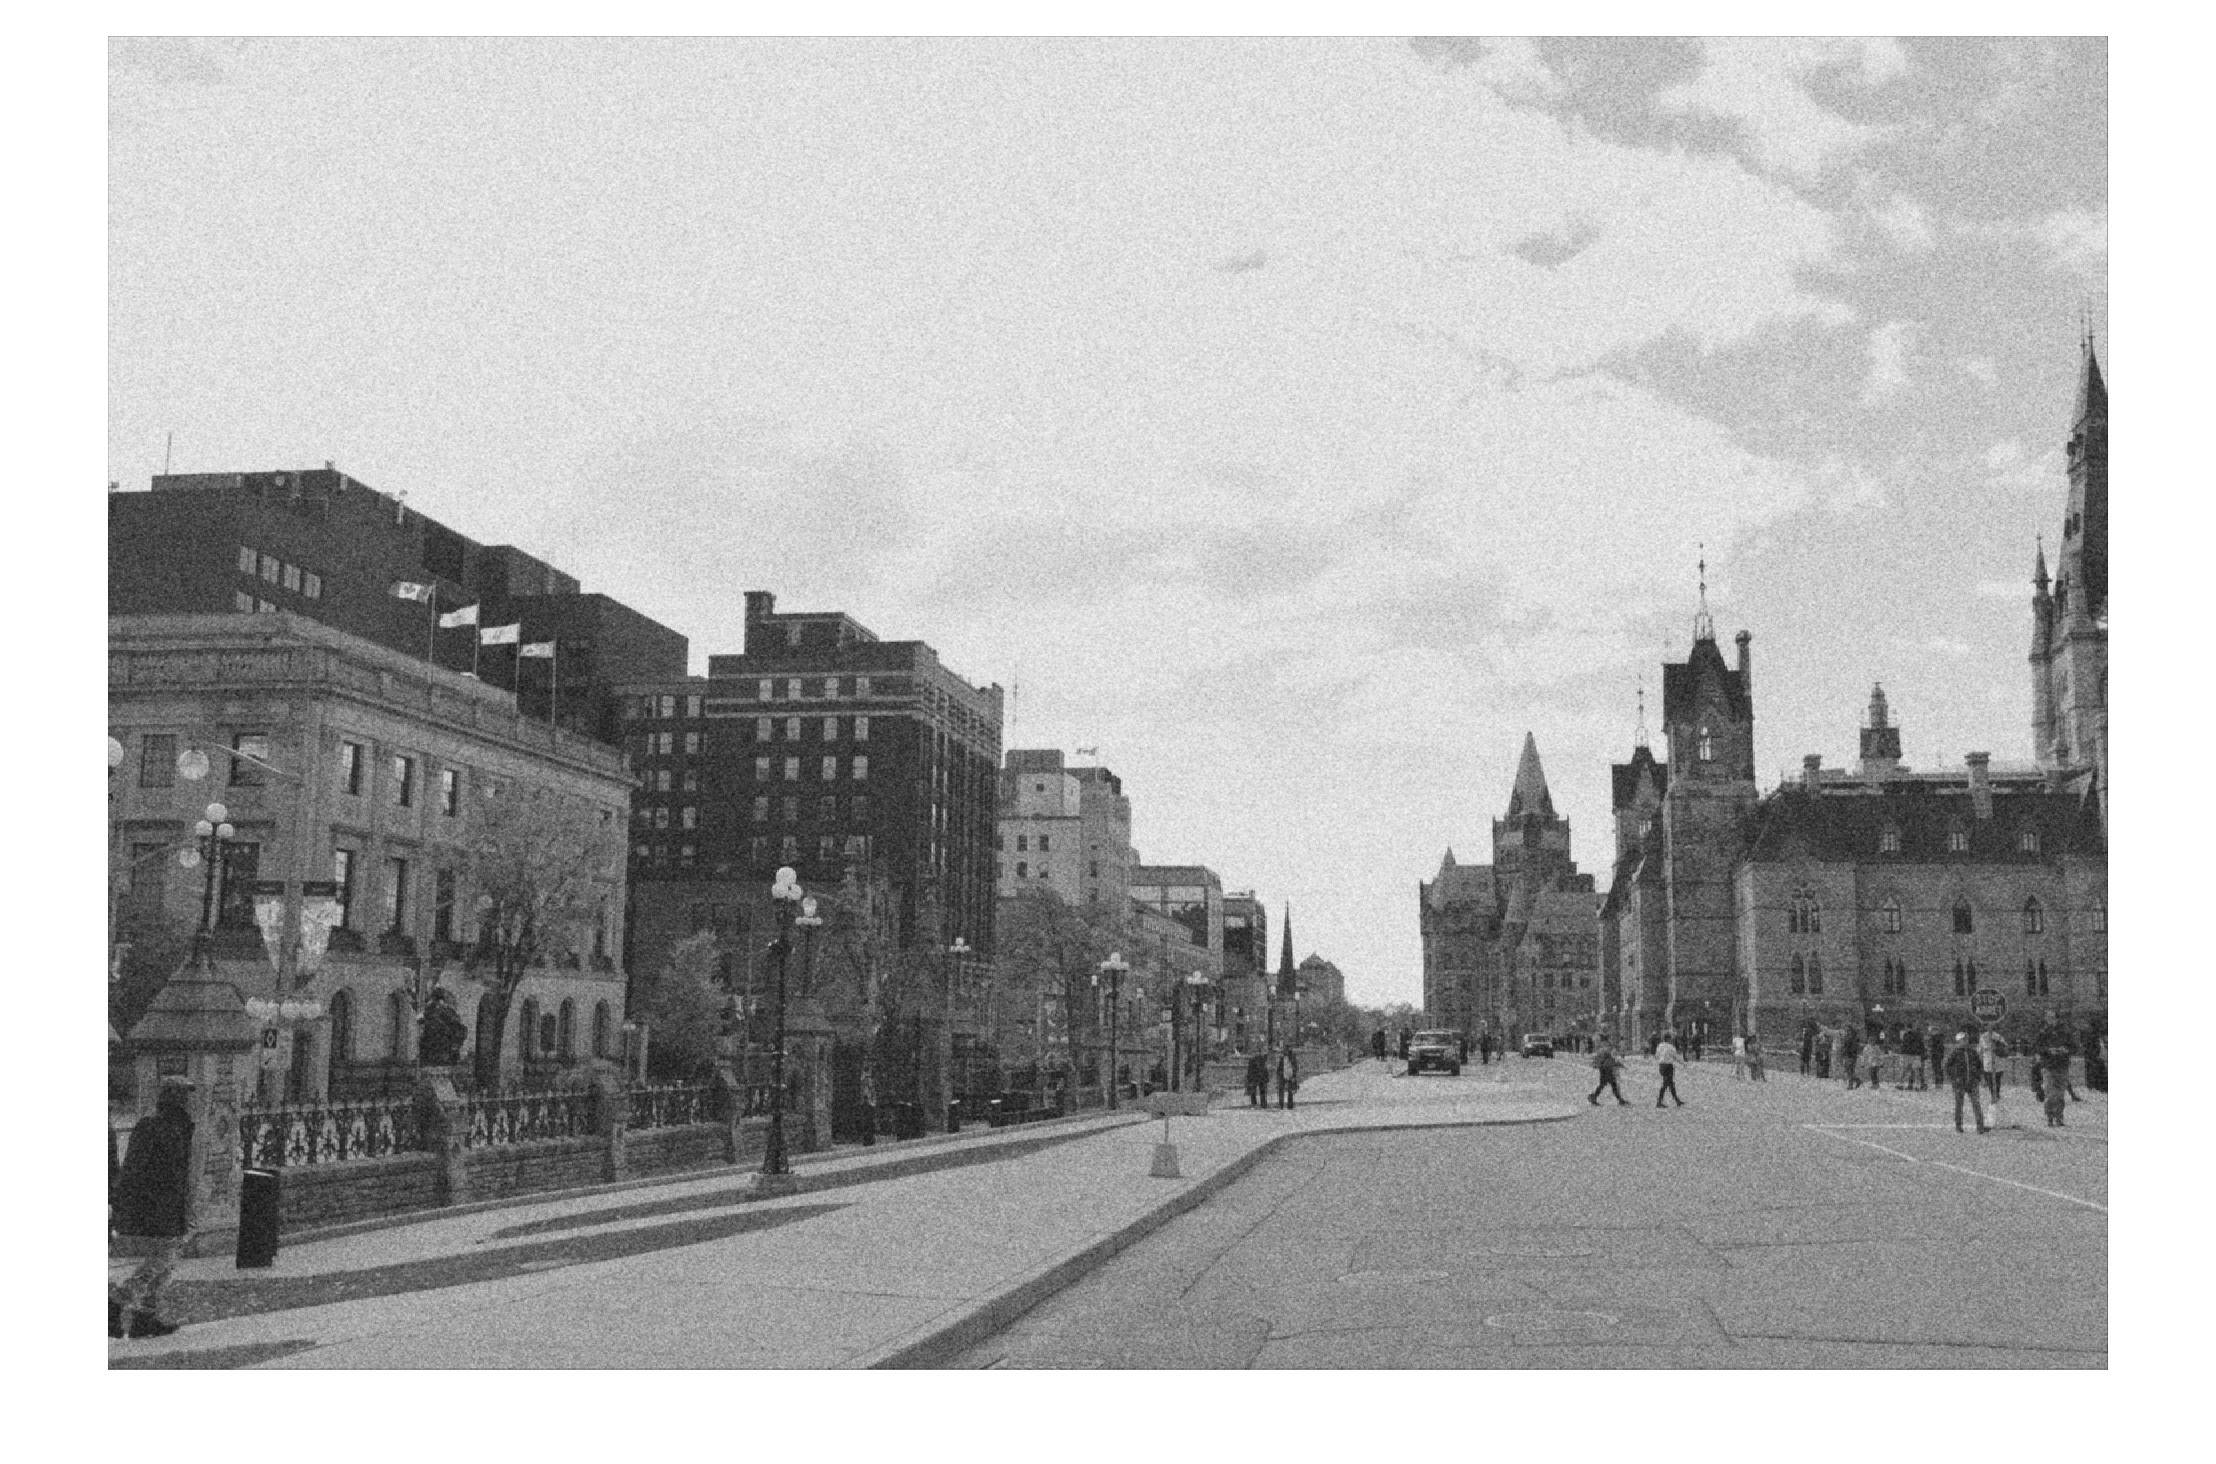
\includegraphics[width=\linewidth]{images/img18.jpg}
\caption{Average filter}
\end{subfigure}
\begin{subfigure}[b]{0.3\linewidth}
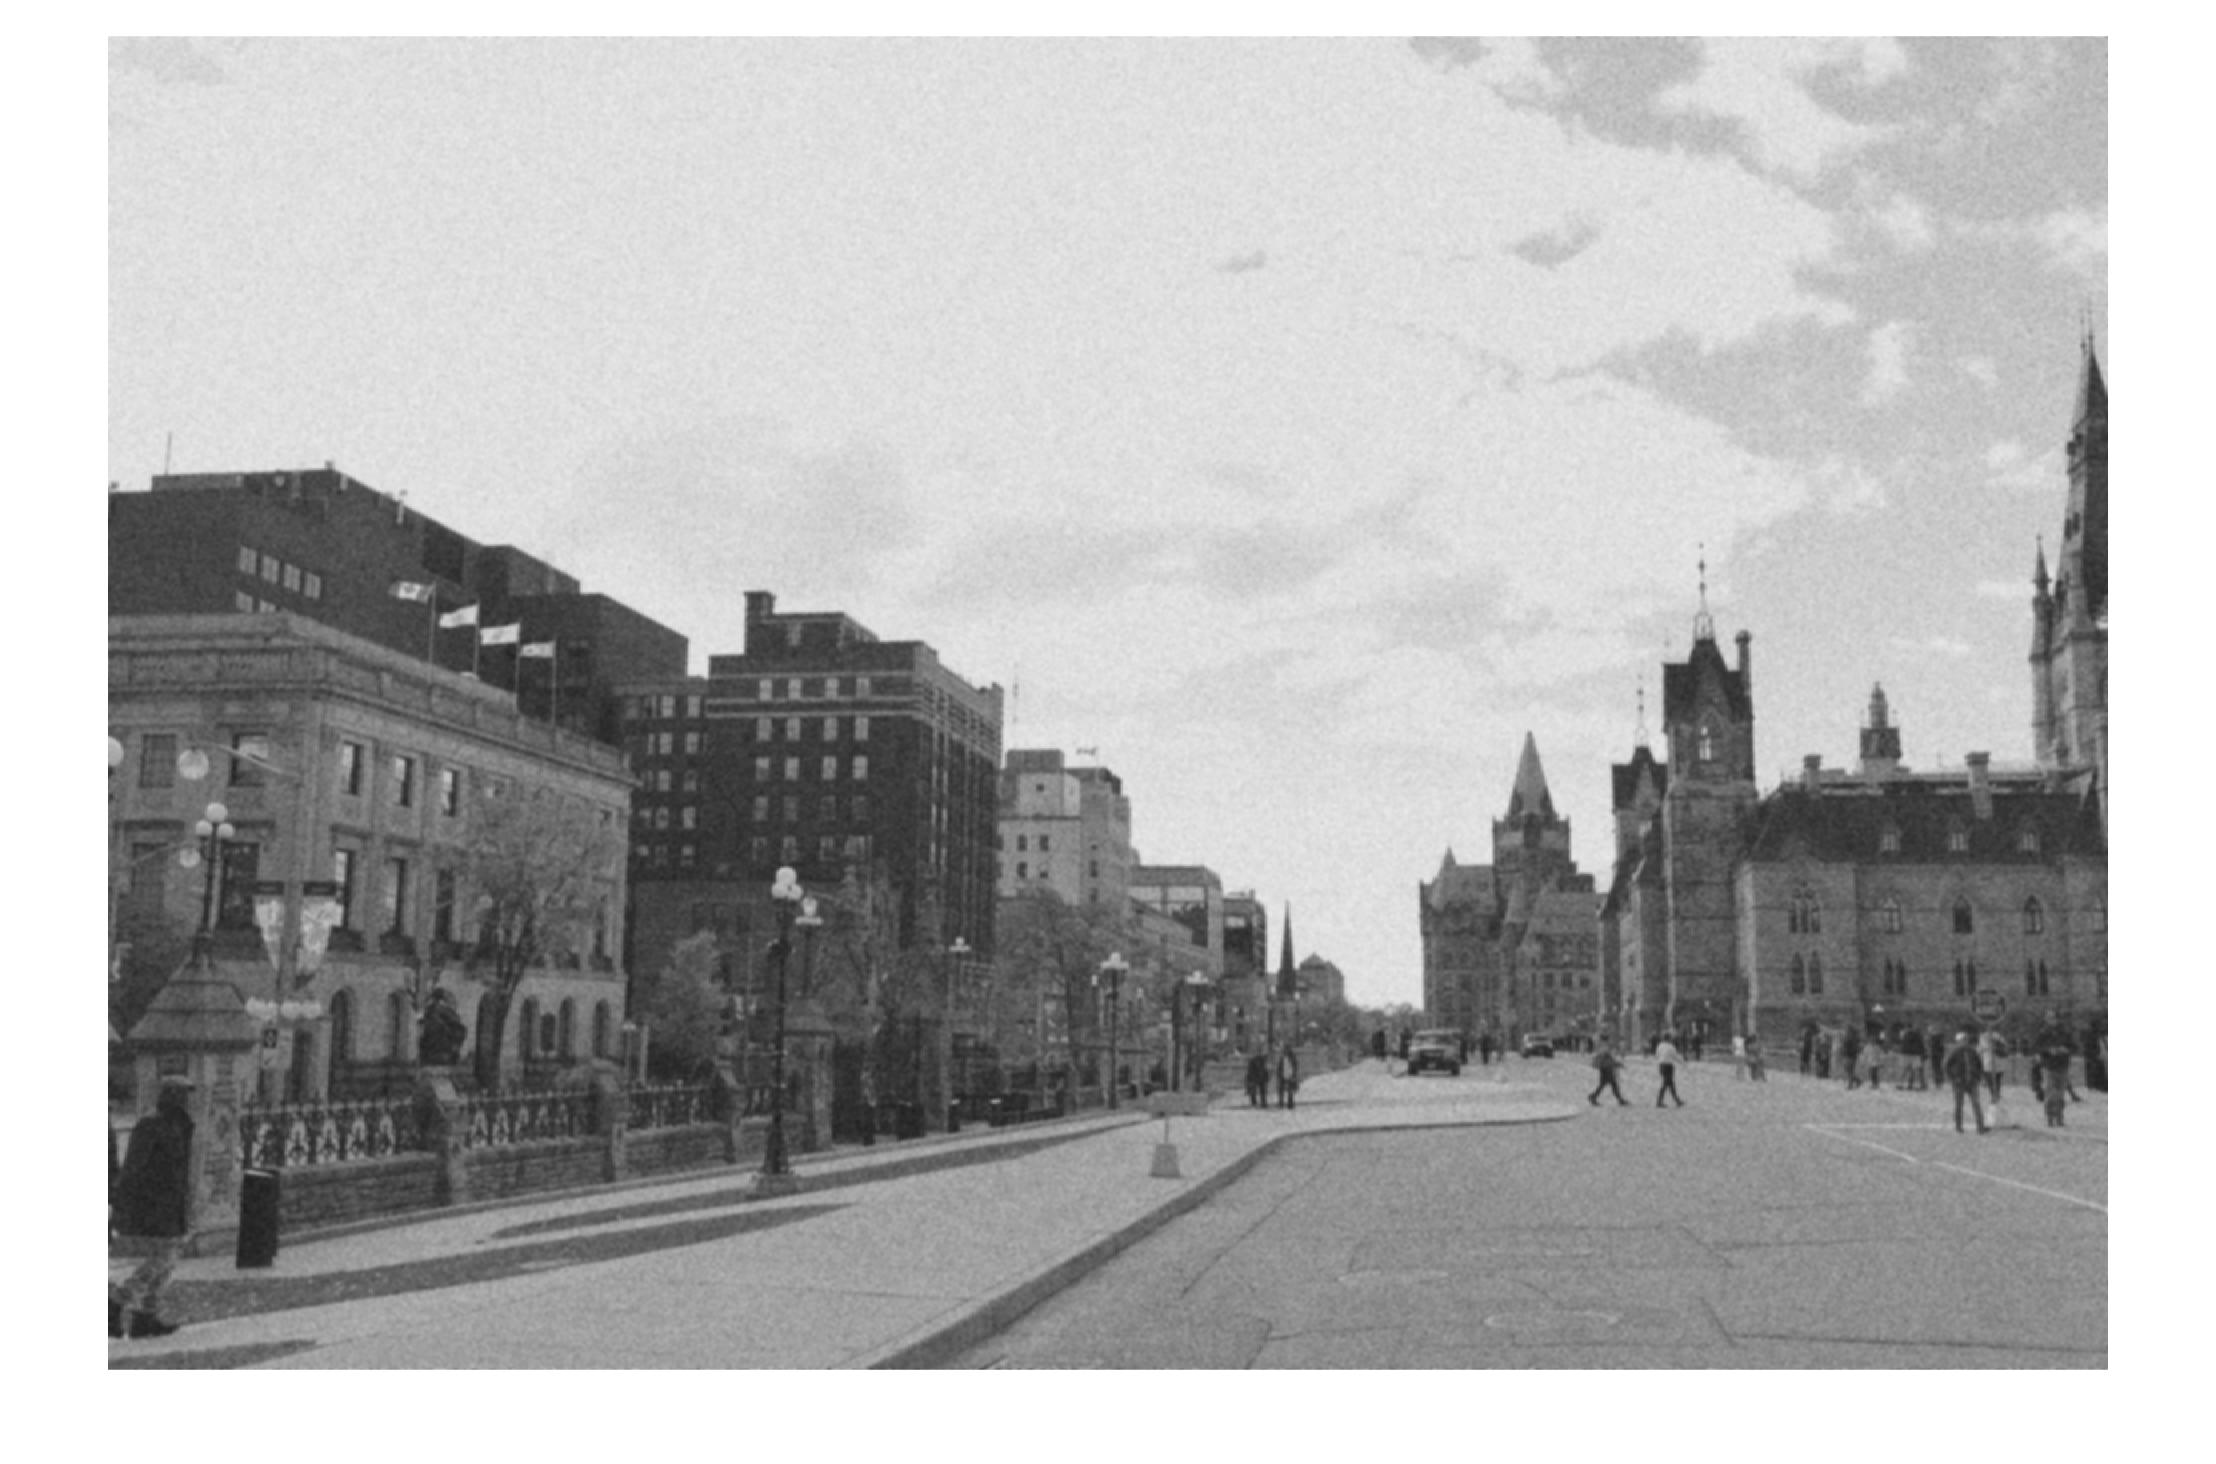
\includegraphics[width=\linewidth]{images/img20.jpg}
\caption{Gaussian filter}
\end{subfigure}
\caption{Applying filters to the image with more noise}
\label{fig:more noise image}
\end{figure}

For the image with lots of noise, a 7x7 average filter and a Gaussian filter with standard deviation of 5 were used. However, it was more effective at smoothing image. Specifically, the resulting images were blurred and the noise was not significantly reduced. 

\clearpage

\subsection{Problem 5}

The \(1^{st}\) derivative function of an 2D image as function \(f(x,y)\) is 

\[ {\frac{\partial f}{\partial x}} = f(x + 1,y) - f(x,y) \]


\[ {\frac{\partial f}{\partial y}} = f(x,y + 1) - f(x,y) \]

The \(2^{nd}\) derivative function is as follow 

\[ {\frac{\partial^2 f}{\partial x^2}} = f(x - 1,y) + f(x + 1,y) - 2f(x,y) \]

\[ {\frac{\partial^2 f}{\partial y^2}} = f(x,y - 1) + f(x,y + 1) - 2f(x,y) \]

The Laplacian is implemented as follow

\[ {\nabla}^2f = {\frac{\partial^2 f}{\partial x^2}} + {\frac{\partial^2 f}{\partial y^2}}\]

\[ {\nabla}^2f = f(x - 1,y) + f(x + 1,y) + f(x,y - 1) + f(x,y + 1) - 4f(x,y) \]

Compute the \(1^{st}\) derivative of the following 3-bit image: \\

\begin{tabularx}{0.2\textwidth} { 
  | >{\centering\arraybackslash}X
  | >{\centering\arraybackslash}X
  | >{\centering\arraybackslash}X
  | >{\centering\arraybackslash}X 
  | >{\centering\arraybackslash}X | }
 \hline
 0 & 2 & 5 & 7 \\
 \hline
 2 & 5 & 7 & 3 \\
 \hline
 5 & 6 & 3 & 1 \\
 \hline
 5 & 2 & 1 & 0 \\
\hline
\end{tabularx} \\

Sample calculation for \(1^{st}\) derivative in x direction:
\[ {\frac{\partial f}{\partial x}} = f(x + 1,y) - f(x,y) = 2 - 0 = 2\]

\(1^{st}\) derivative in x direction: \\

\begin{tabularx}{0.2\textwidth} { 
  | >{\centering\arraybackslash}X
  | >{\centering\arraybackslash}X
  | >{\centering\arraybackslash}X
  | >{\centering\arraybackslash}X 
  | >{\centering\arraybackslash}X | }
 \hline
 2 & 3 & 2 &  \\
 \hline
 3 & 2 & -4 &  \\
 \hline
 1 & -3 & -2 &  \\
 \hline
 -3 & -1 & -1 &  \\
\hline
\end{tabularx} \\

Sample calculation for \(1^{st}\) derivative in y direction:
\[ {\frac{\partial f}{\partial y}} = f(x,y + 1) - f(x,y) = 0 - 2 = -2\]

\(1^{st}\) derivative in y direction: \\

\begin{tabularx}{0.2\textwidth} { 
  | >{\centering\arraybackslash}X
  | >{\centering\arraybackslash}X
  | >{\centering\arraybackslash}X
  | >{\centering\arraybackslash}X 
  | >{\centering\arraybackslash}X | }
 \hline
  &  &  &  \\
 \hline
 -2 & -3 & -2 & 4 \\
 \hline
 -3 & -1 & 4 & 2 \\
 \hline
 0 & 4 & 2 & 1 \\
\hline
\end{tabularx} \\

The image after applying Laplacian mask: \\

\begin{tabularx}{0.3\textwidth} { 
  | >{\centering\arraybackslash}X
  | >{\centering\arraybackslash}X
  | >{\centering\arraybackslash}X
  | >{\centering\arraybackslash}X 
  | >{\centering\arraybackslash}X | }
 \hline
 4 & 2 & -4 & -20 \\
 \hline
 2 & -3 & -12 & 3 \\
 \hline
 -7 & -9 & 3 & 2 \\
 \hline
 -13 & 4 & 1 & 2 \\
\hline
\end{tabularx} \\

The result after normalization: \\

\begin{tabularx}{0.3\textwidth} { 
  | >{\centering\arraybackslash}X
  | >{\centering\arraybackslash}X
  | >{\centering\arraybackslash}X
  | >{\centering\arraybackslash}X 
  | >{\centering\arraybackslash}X | }
 \hline
 0.94 & 0.60 & -0.15 & -1.50 \\
 \hline
 0.69 & -0.26 & -1.35 & 0.56 \\
 \hline
 -0.44 & -1.29 & 0.90 & 0.47 \\
 \hline
 -1.20 & 0.95 & 0.60 & 0.47 \\
\hline
\end{tabularx} \\

\clearpage
\section{Part 2}
\subsection{Brief Description of Image Enhancement Algorithm}

Enhancements are used to make imagery easier to understand and interpret visually. The ability to change an image's digital pixel values is a benefit of using digital images. The image may still not be ideal for visual interpretation even after radiometric corrections for illumination, atmospheric factors, and sensor characteristics have been made before data delivery to the user. As a result, it is typically essential to change the range and distribution of brightness values specifically for each application and each image.

In raw images, the relevant data frequently only fills a small percentage of the range of digital values that are available (commonly 8 bits or 256 levels). By altering the initial values, more of the available range can be utilised, enhancing the contrast between the backgrounds of targets and their backgrounds. Understanding the idea of an image histogram is essential to comprehending contrast enhancements. A histogram is a graphical representation of an image's brightness levels. Along the graph's x-axis are the brightness levels (from 0-255). The y-axis displays the frequency of occurrence of each of these values in the image.

The histogram of a picture serves as a graphic representation of the image's digital value range, which can be changed to apply different data upgrades. We'll only touch on a few widely used approaches and techniques for improving contrast and detail in an image. A linear contrast stretch is the most straightforward enhancement type. Identifying the histogram's lower and upper bounds—typically the image's minimum and maximum brightness values—and then using a transformation to expand this range to encompass the entire range are necessary to do this. Our example's histogram has a minimum value of 84 and a maximum value of 153, both of which are populated by actual data. Compared to the total 256 levels accessible, these 70 levels only take up about a third of the space. This narrow range is consistently expanded by a linear stretch to include the entire range of values from 0 to 255. With light tones seeming lighter and dark tones appearing darker, the contrast in the image is improved, making visual interpretation considerably simpler.

In this assignment, the low-light image enhancement technique will be investigated. Specifically, these images may have poor dynamic ranges and excessive noise levels, which can negatively impact how well computer vision algorithms work in general. Use low-light image enhancement to boost an image's visibility in order to make computer vision algorithms resilient in dim lighting. The histogram of hazy photographs is quite similar to the histogram of low-light or HDR images that have had their pixels reversed. So a effective method to improve low-light photographs is the haze reduction techniques.

\subsection{Enhance Low Light Image using Dehazing Algorithm}

\begin{lstlisting}[language=Matlab]

% Assignment 2
% Part 2

% Enhance low-light image 
% by dehazing algorithm
% Import an RGB image captured in low light
img = imread('/lamnguyen/Desktop/School/
Computer-Vision/A2/images/church1.jpg');
figure; 
imshow(img);

% Invert the image and 
% notice how the low-light
% areas in the original image appear hazy
inverted_img = imcomplement(img);
figure;
imshow(inverted_img);

% Reduce the haze 
reduced_img = imreducehaze(inverted_img);
figure;
imshow(reduced_img);

% Invert the results to obtain
% the enhanced image
enhanced_img = imcomplement(reduced_img);
figure;
imshow(enhanced_img);

\end{lstlisting}

\begin{figure}[h!]
\centering
\begin{subfigure}[b]{0.4\linewidth}
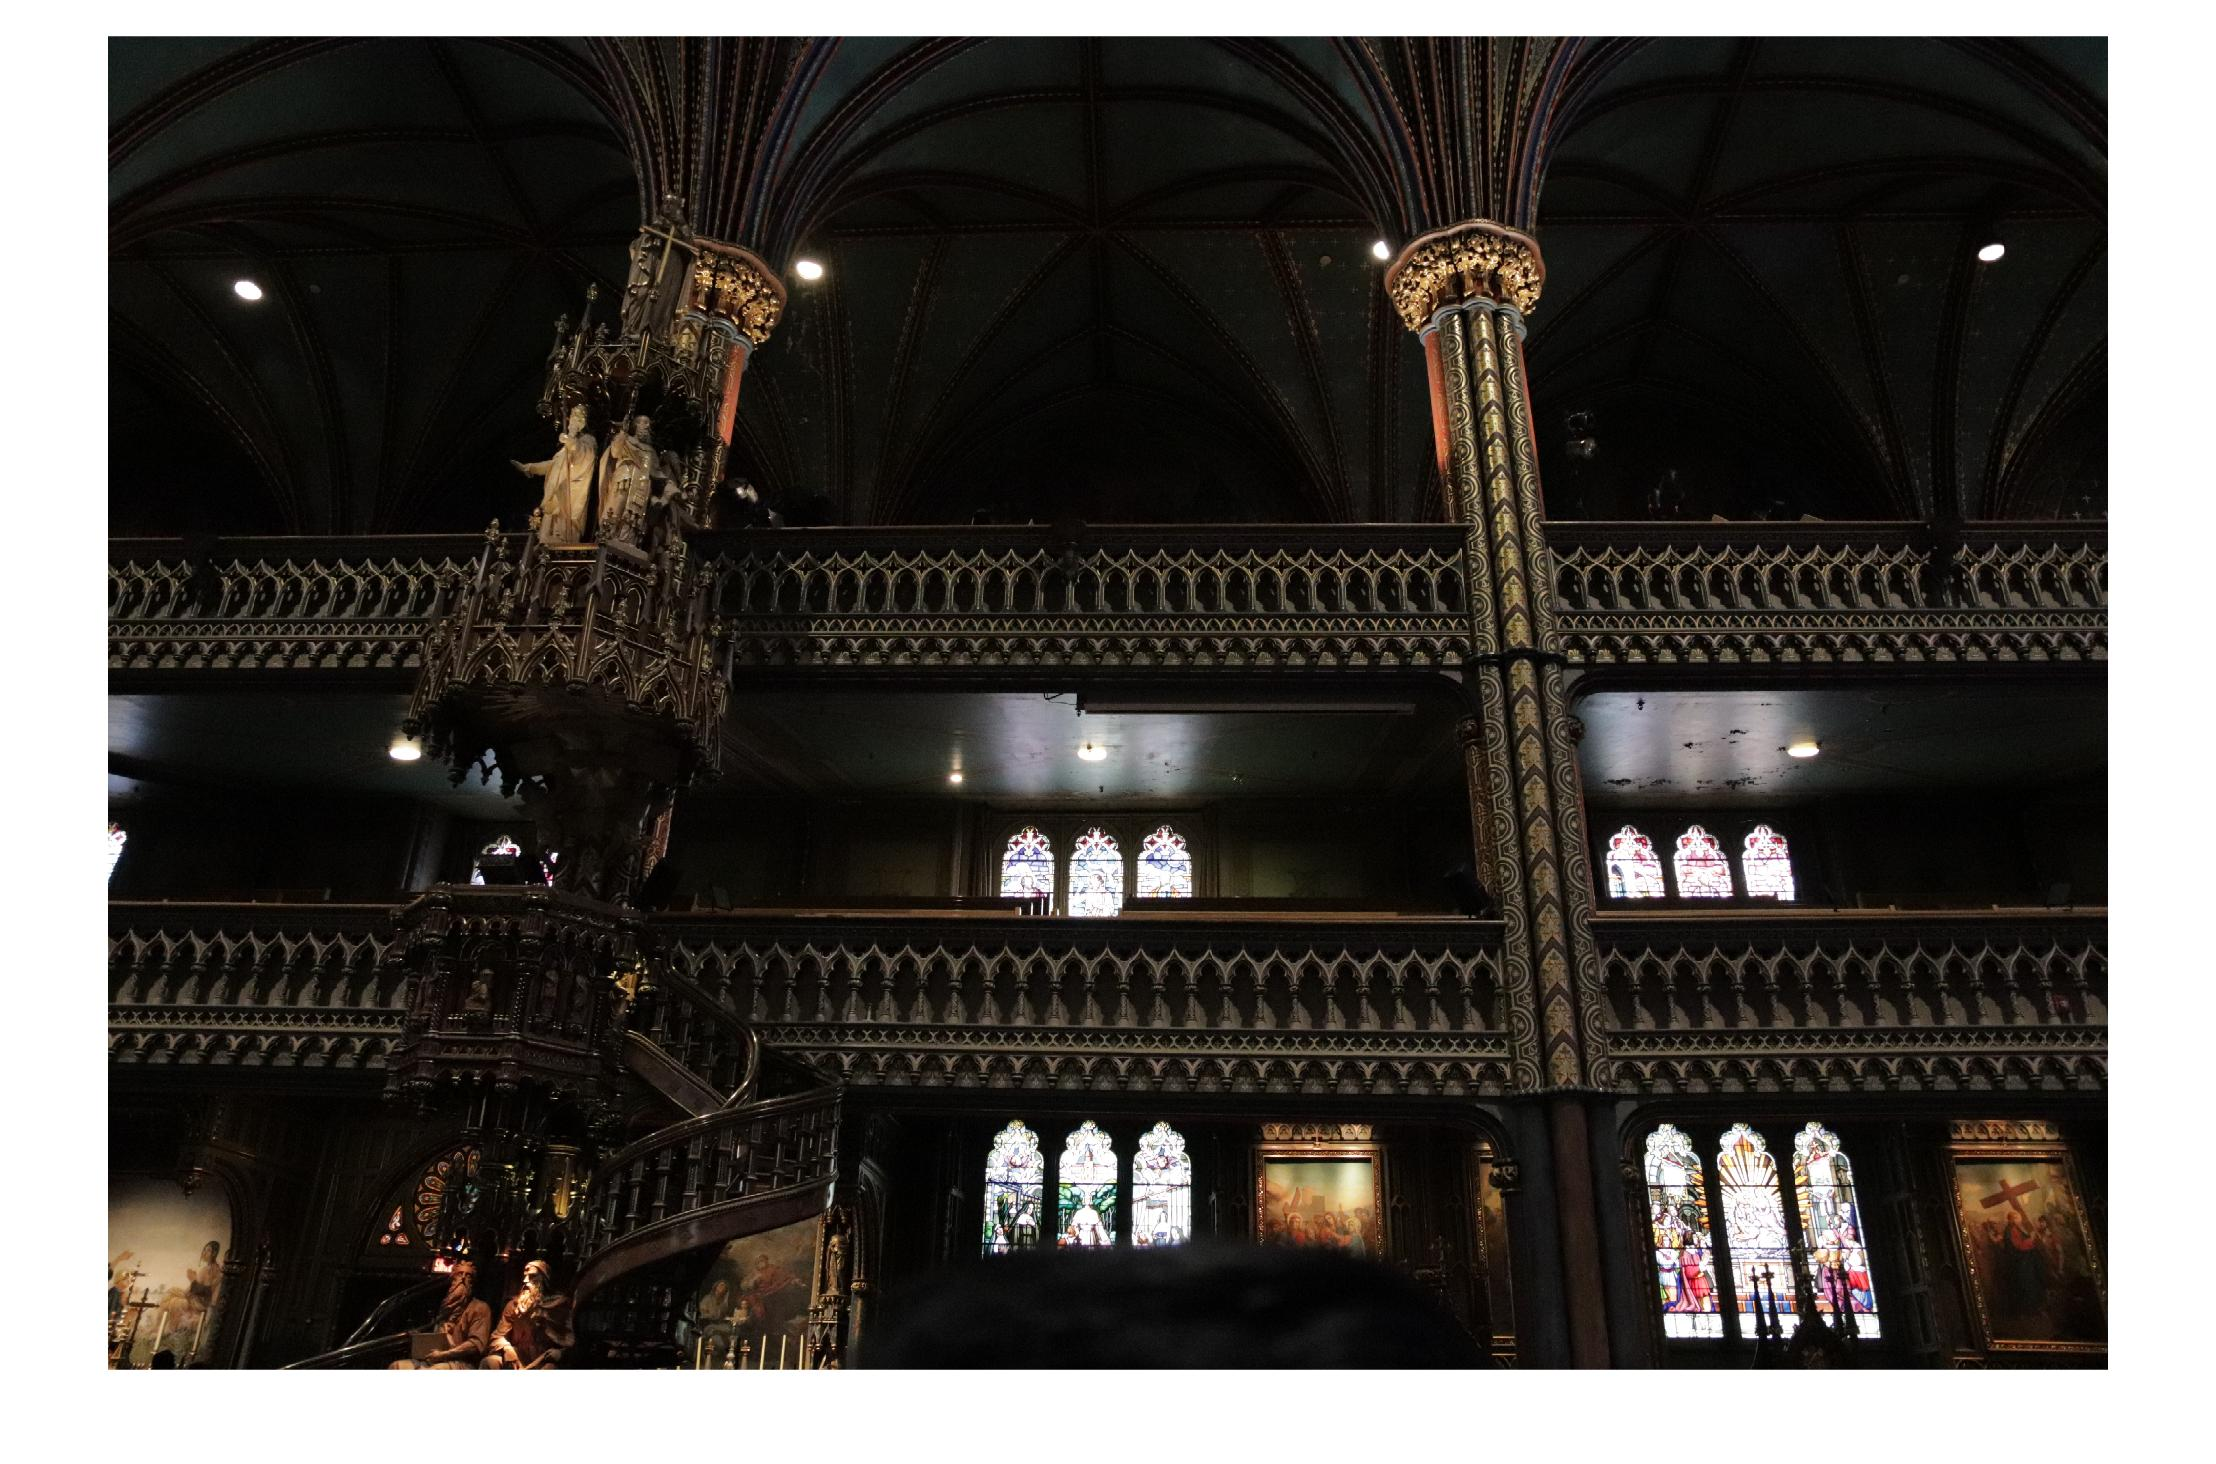
\includegraphics[width=\linewidth]{images/img21.jpg}
\caption{Original image}
\end{subfigure}
\begin{subfigure}[b]{0.4\linewidth}
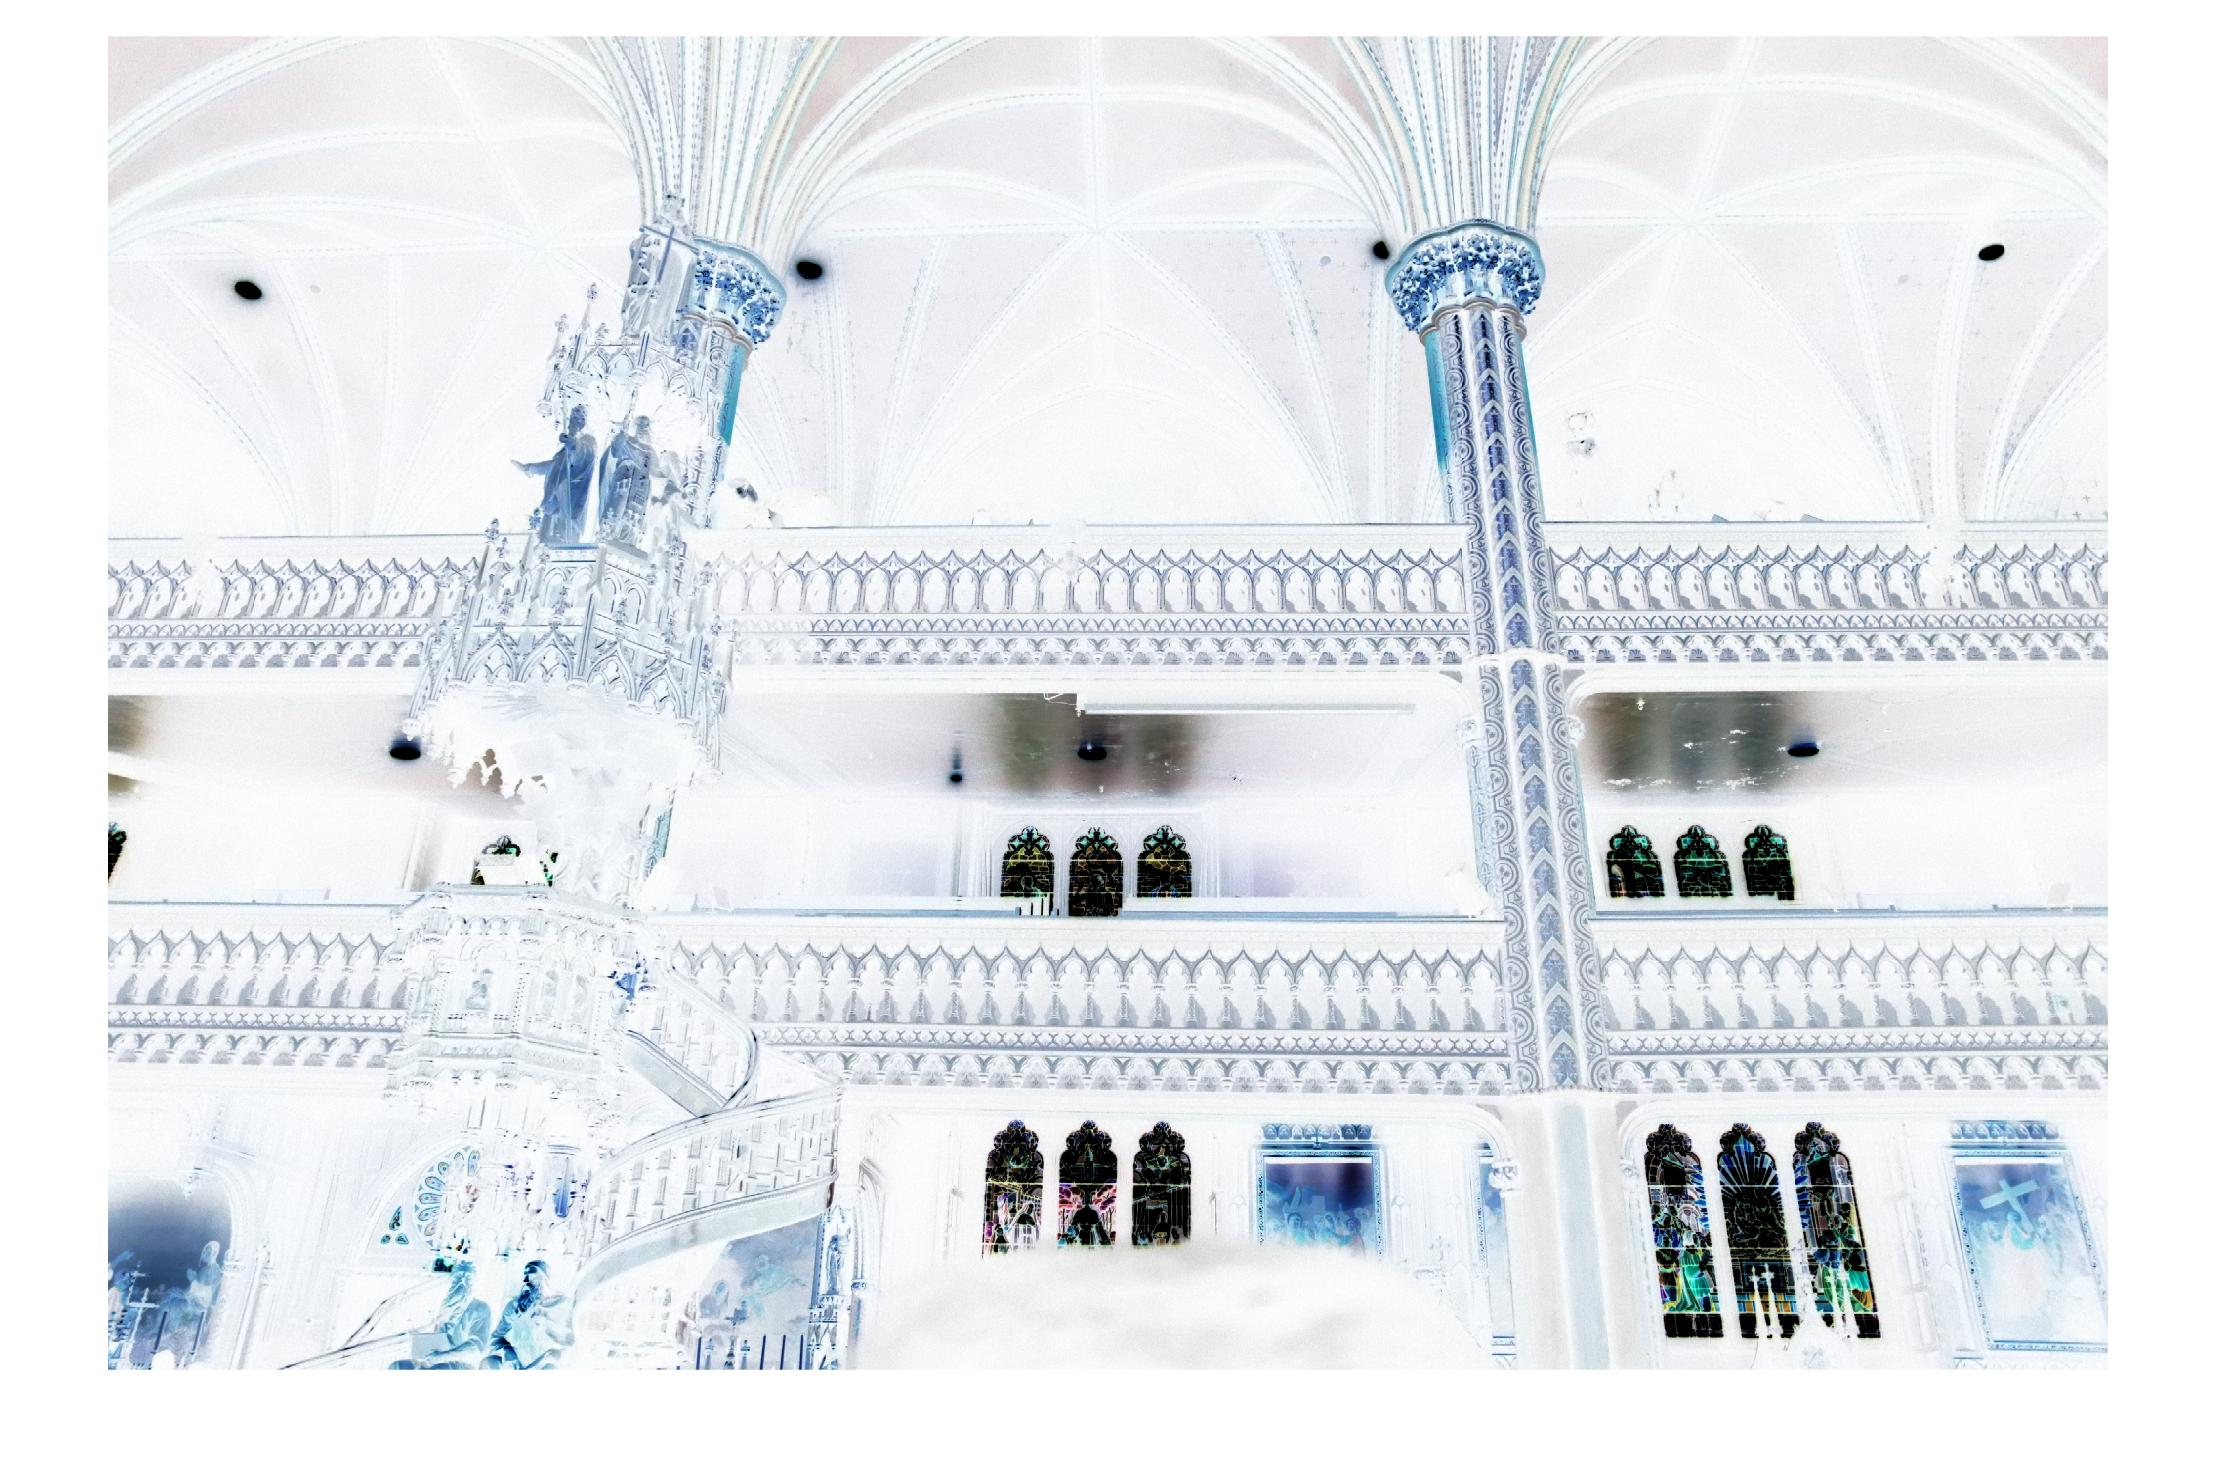
\includegraphics[width=\linewidth]{images/img22.jpg}
\caption{Inverted image}
\end{subfigure}
\begin{subfigure}[b]{0.4\linewidth}
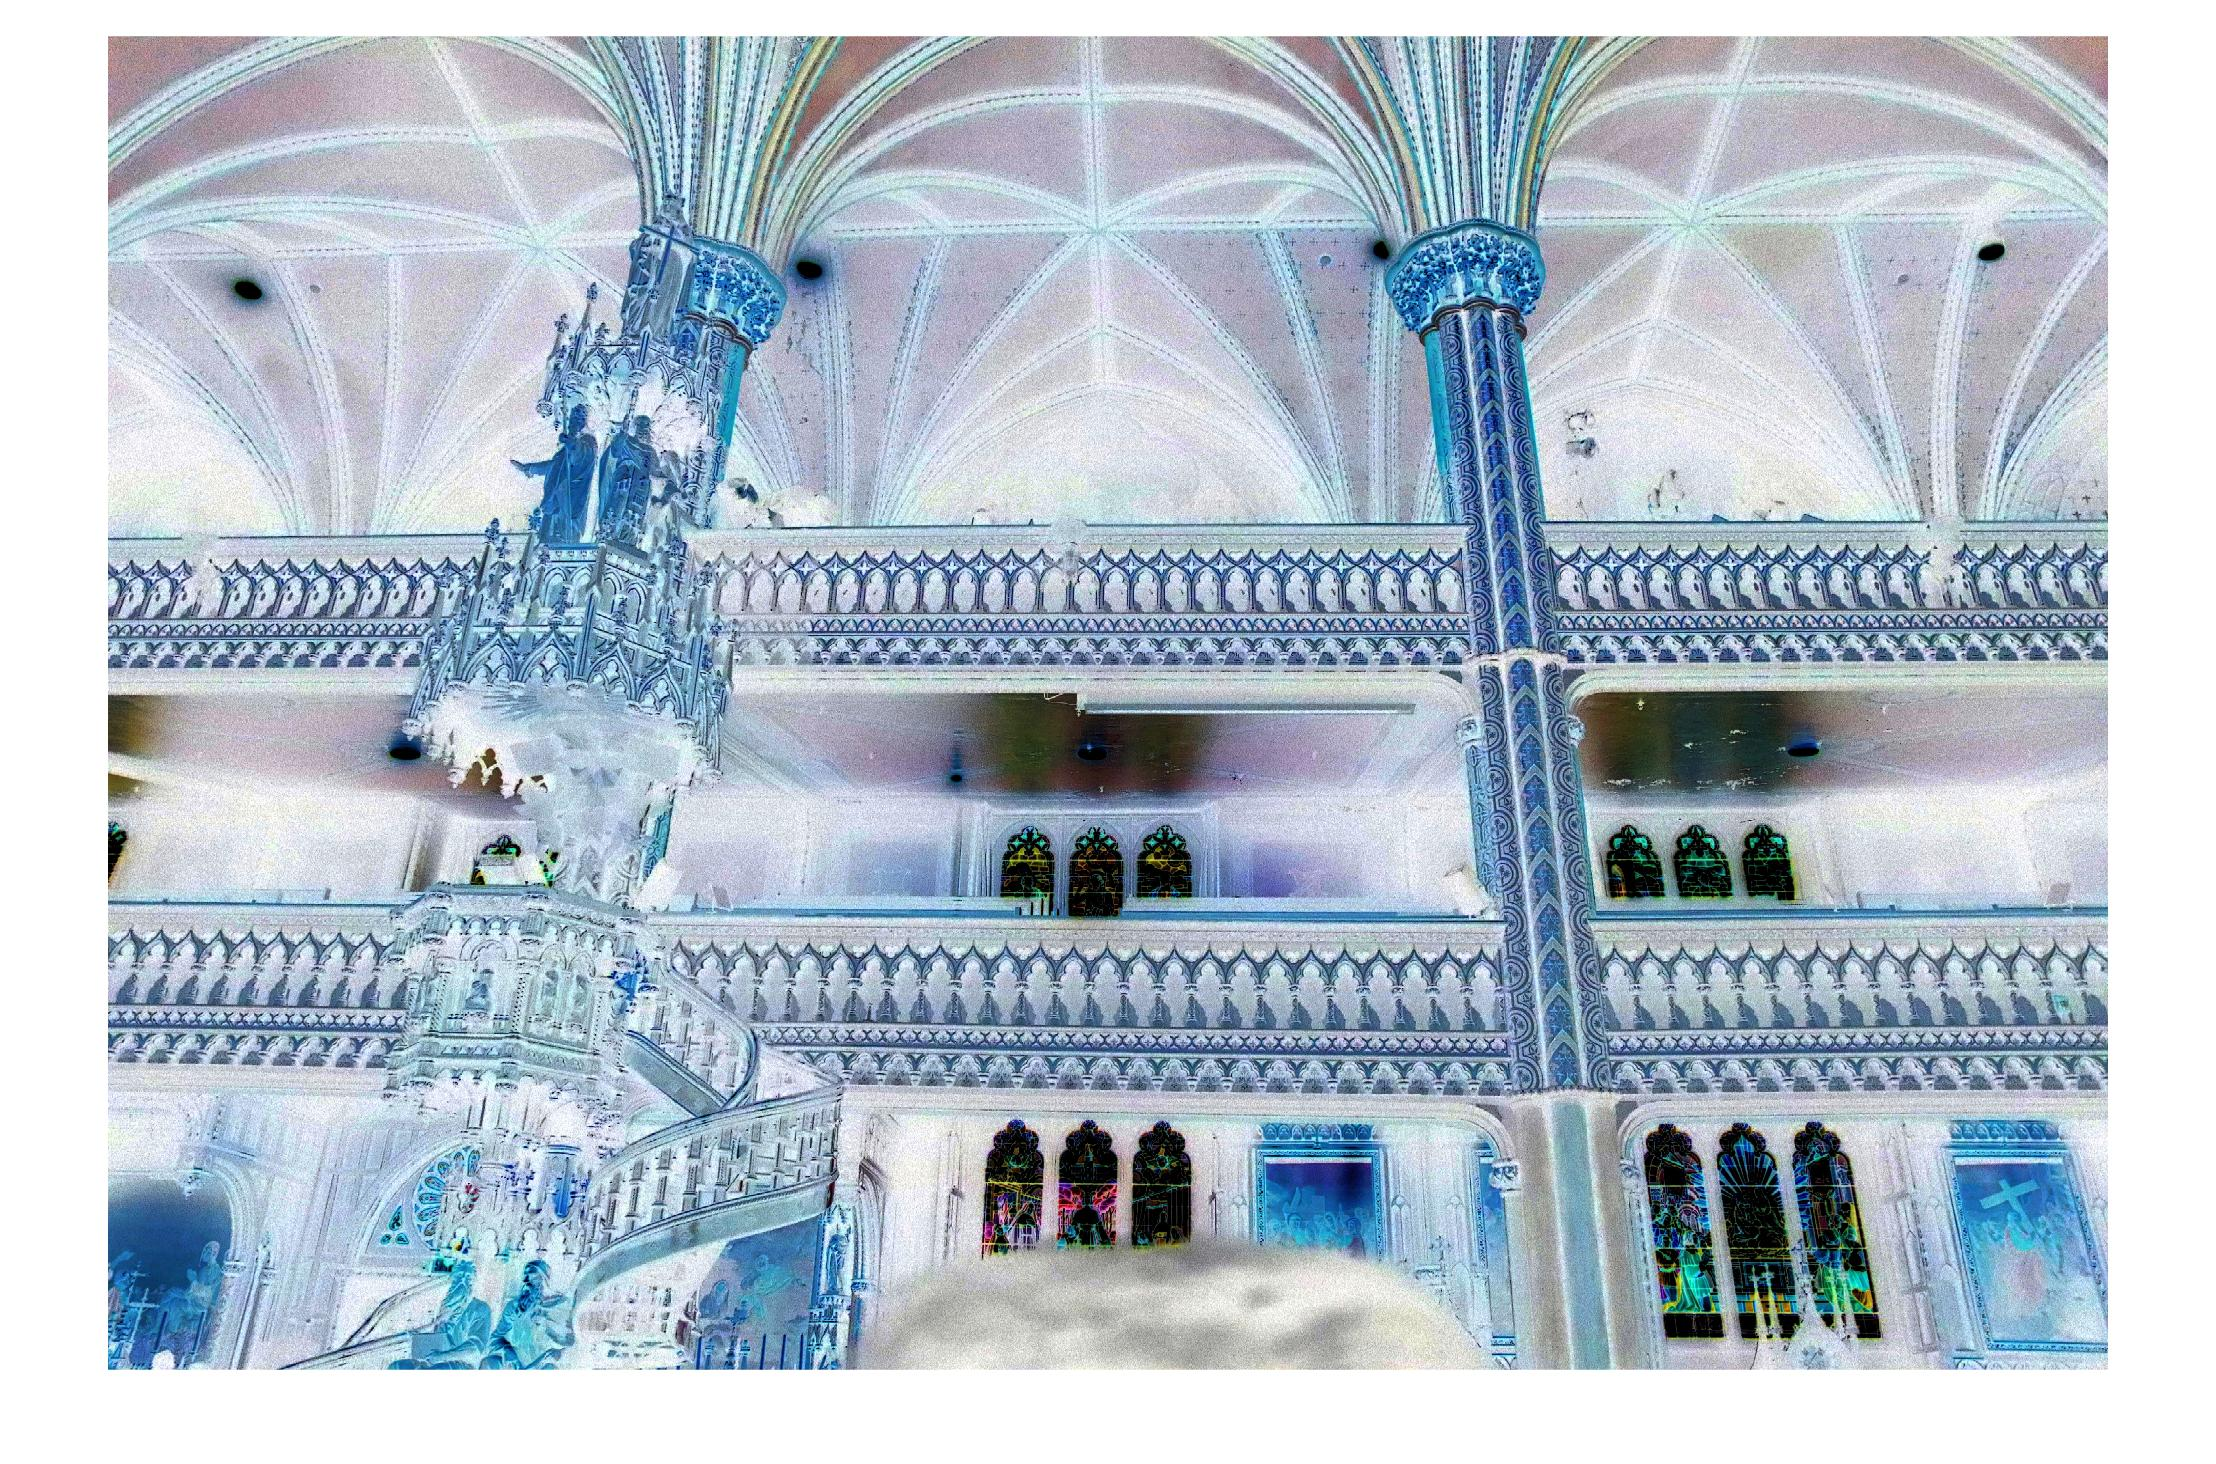
\includegraphics[width=\linewidth]{images/img23.jpg}
\caption{Reduced haze}
\end{subfigure}
\begin{subfigure}[b]{0.4\linewidth}
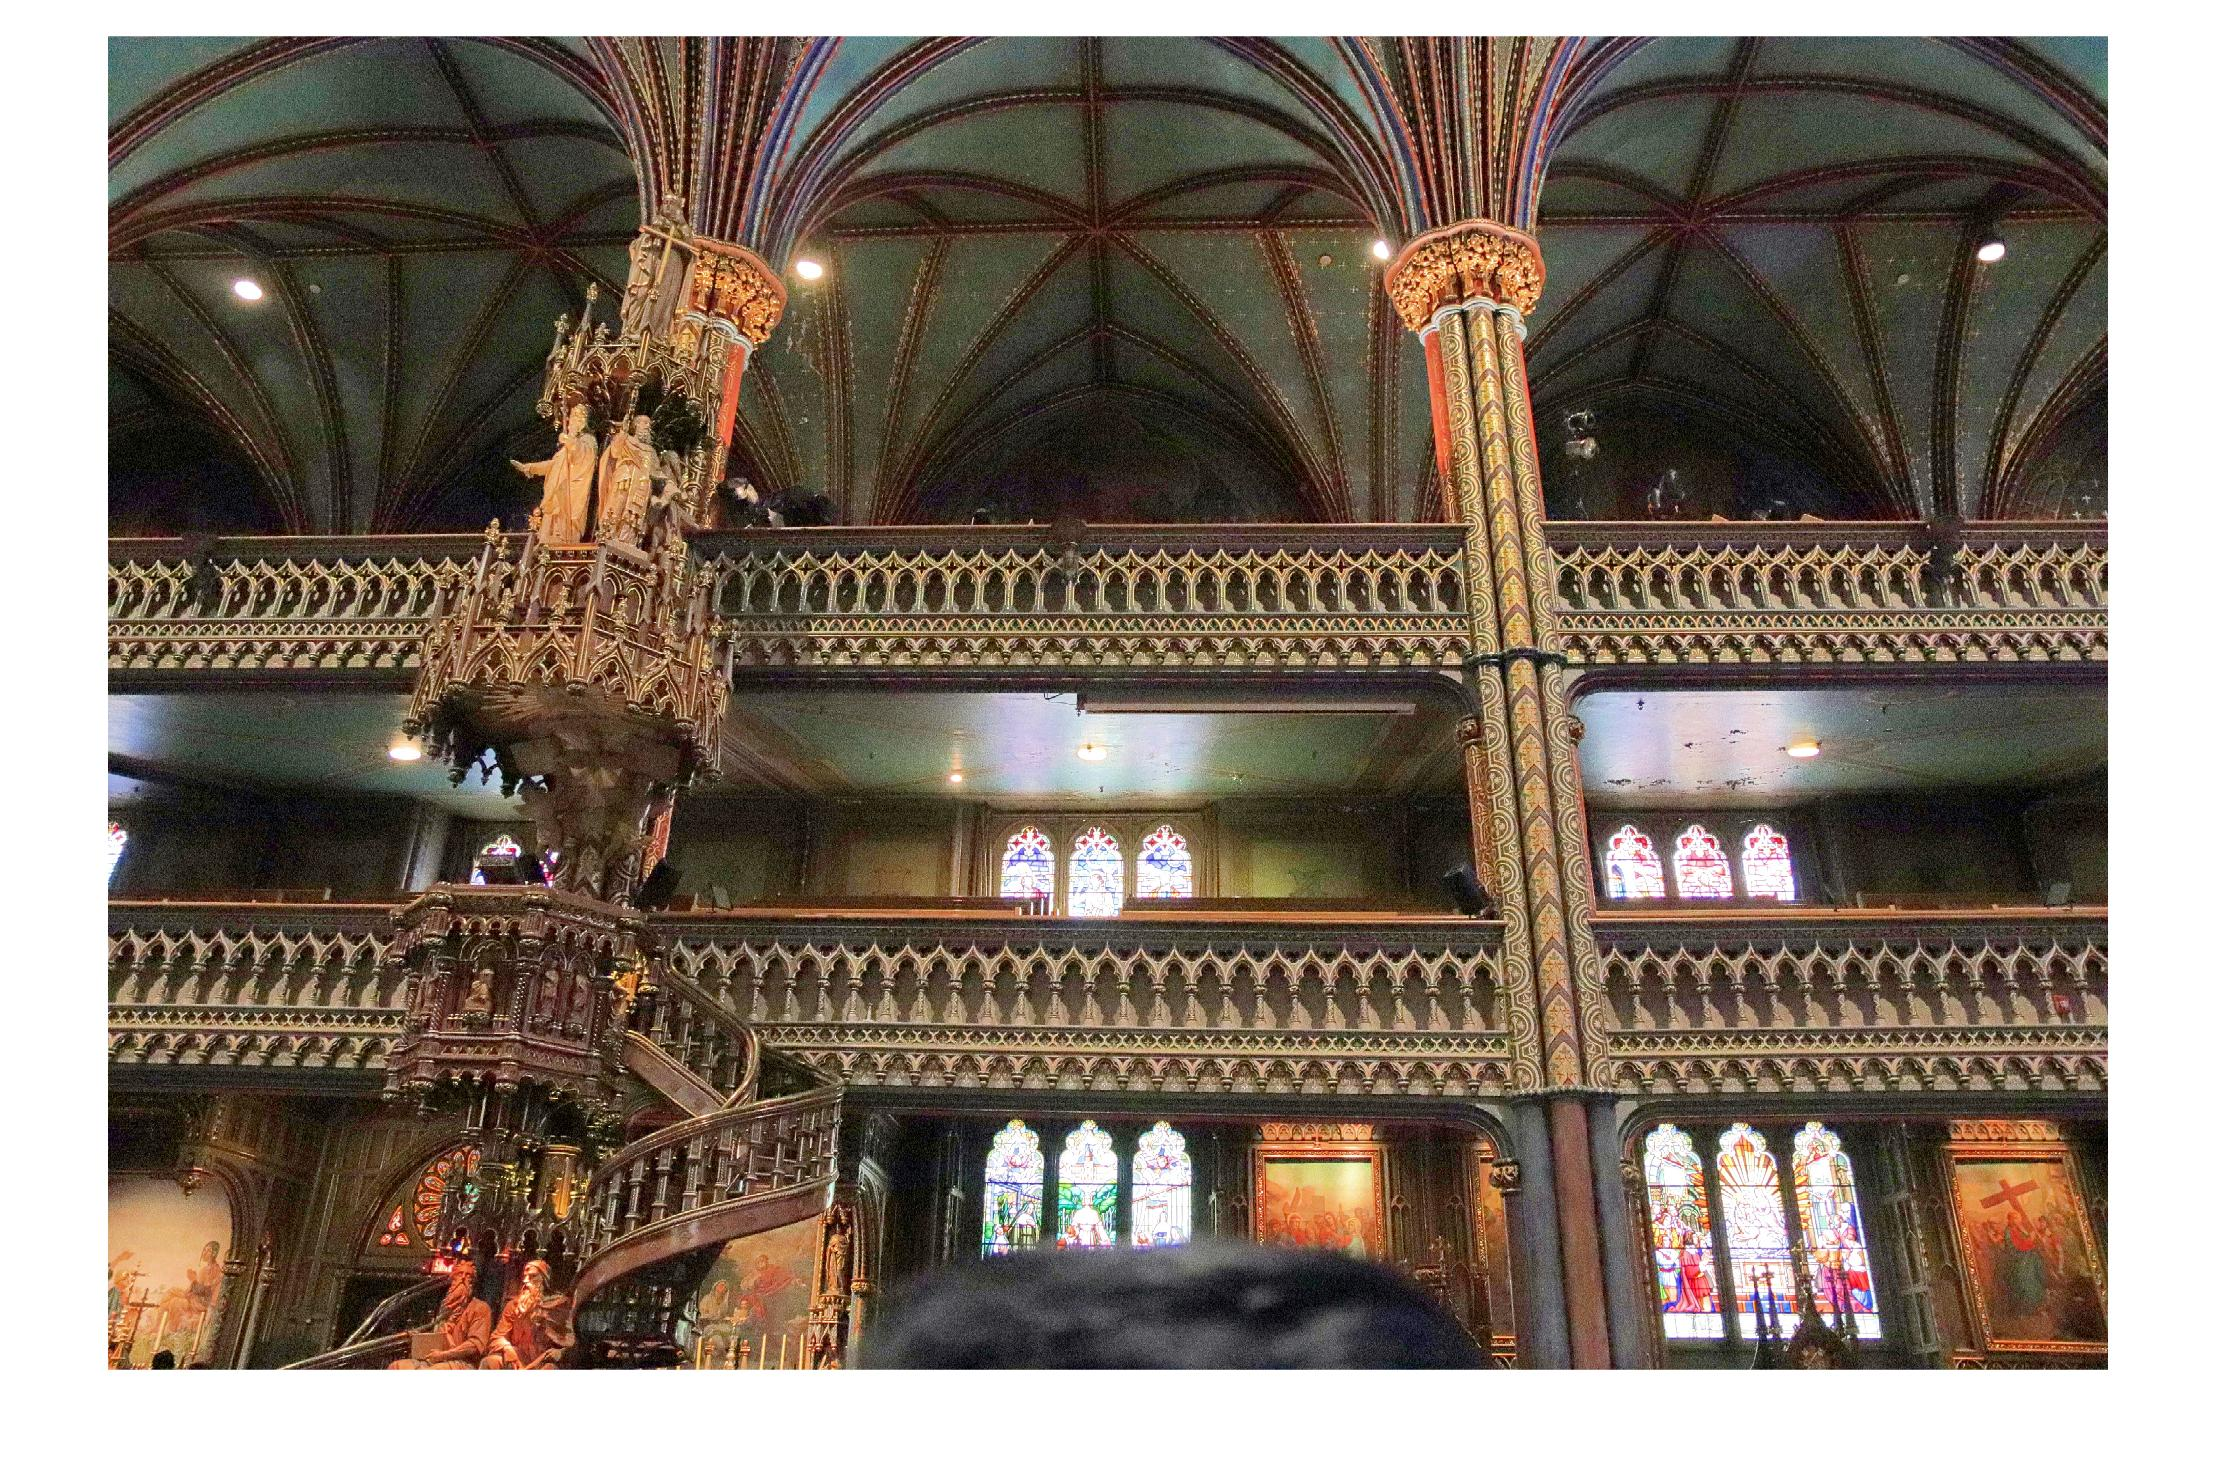
\includegraphics[width=\linewidth]{images/img24.jpg}
\caption{Enhanced image}
\end{subfigure}
\caption{Enhance low-light image by dehazing algorithm}
\label{fig:Enhance low-light image by dehazing algorithm}
\end{figure}

\subsection{Improve Results Further Using 'imreducehaze' Optional Parameters}

\begin{lstlisting}[language=Matlab]

% Improve Results Further Using 
% imreducehaze Optional Parameters
reduced_img = imreducehaze(inverted_img, 
'Method','approx','ContrastEnhancement',
'boost');
improved_img = imcomplement(reduced_img);
figure;
imshow(improved_img);

\end{lstlisting}

\begin{figure}[h!]
\centering
\begin{subfigure}[b]{0.4\linewidth}
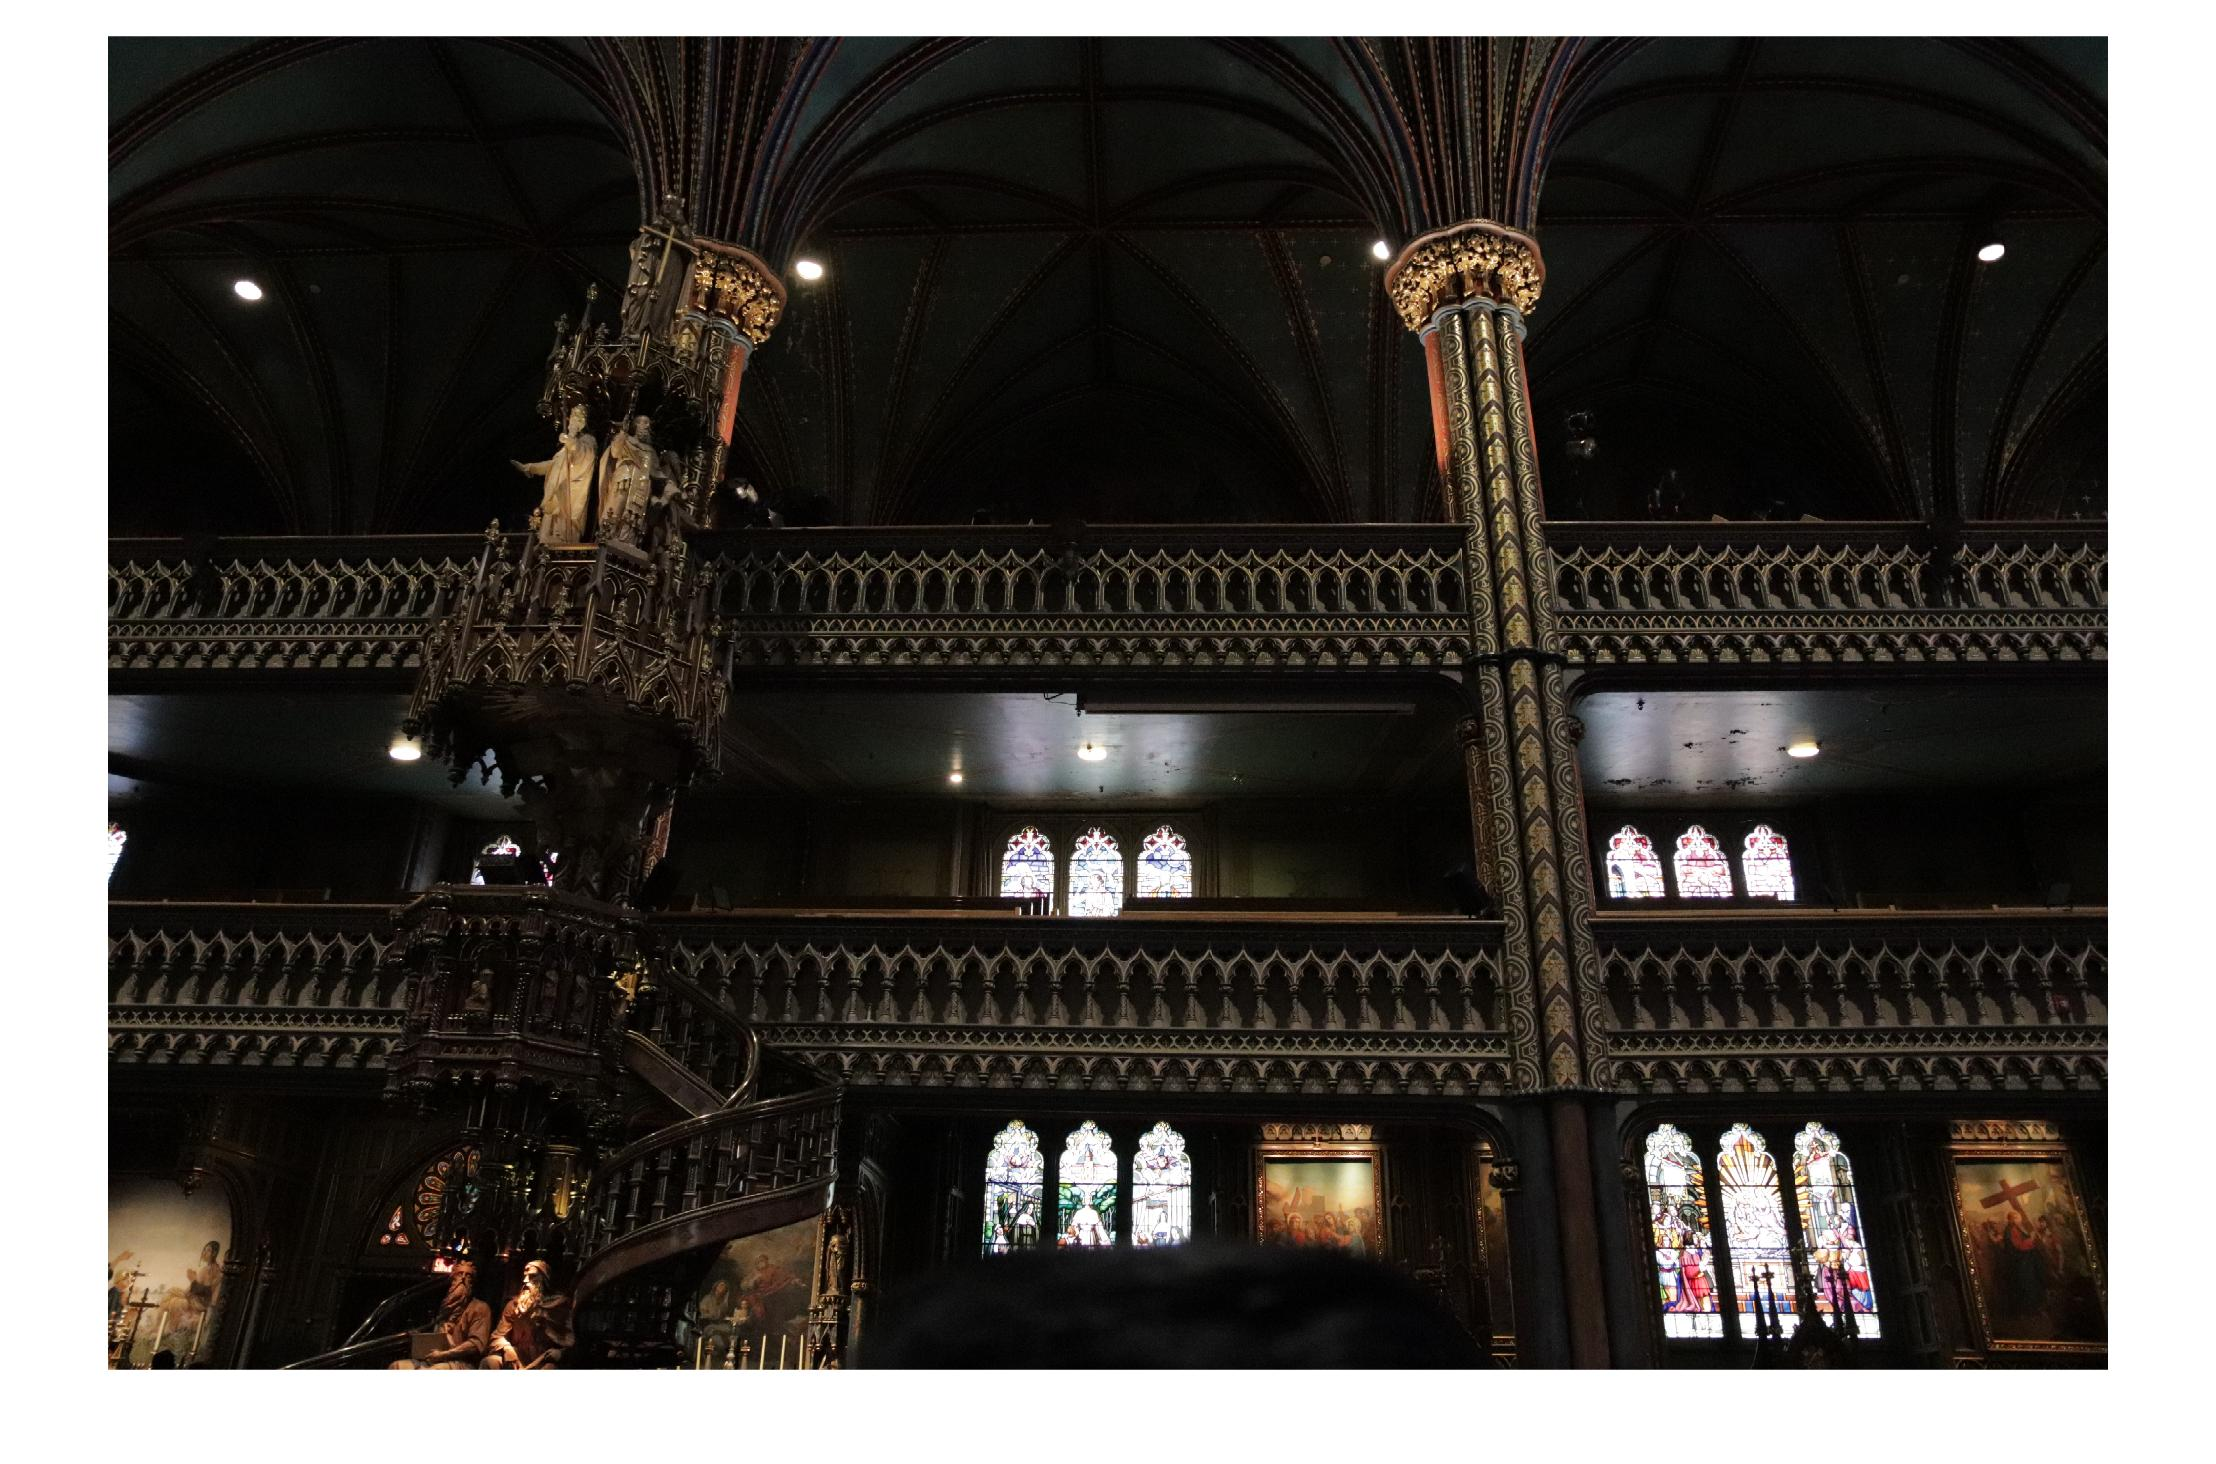
\includegraphics[width=\linewidth]{images/img21.jpg}
\caption{Original image}
\end{subfigure}
\begin{subfigure}[b]{0.4\linewidth}
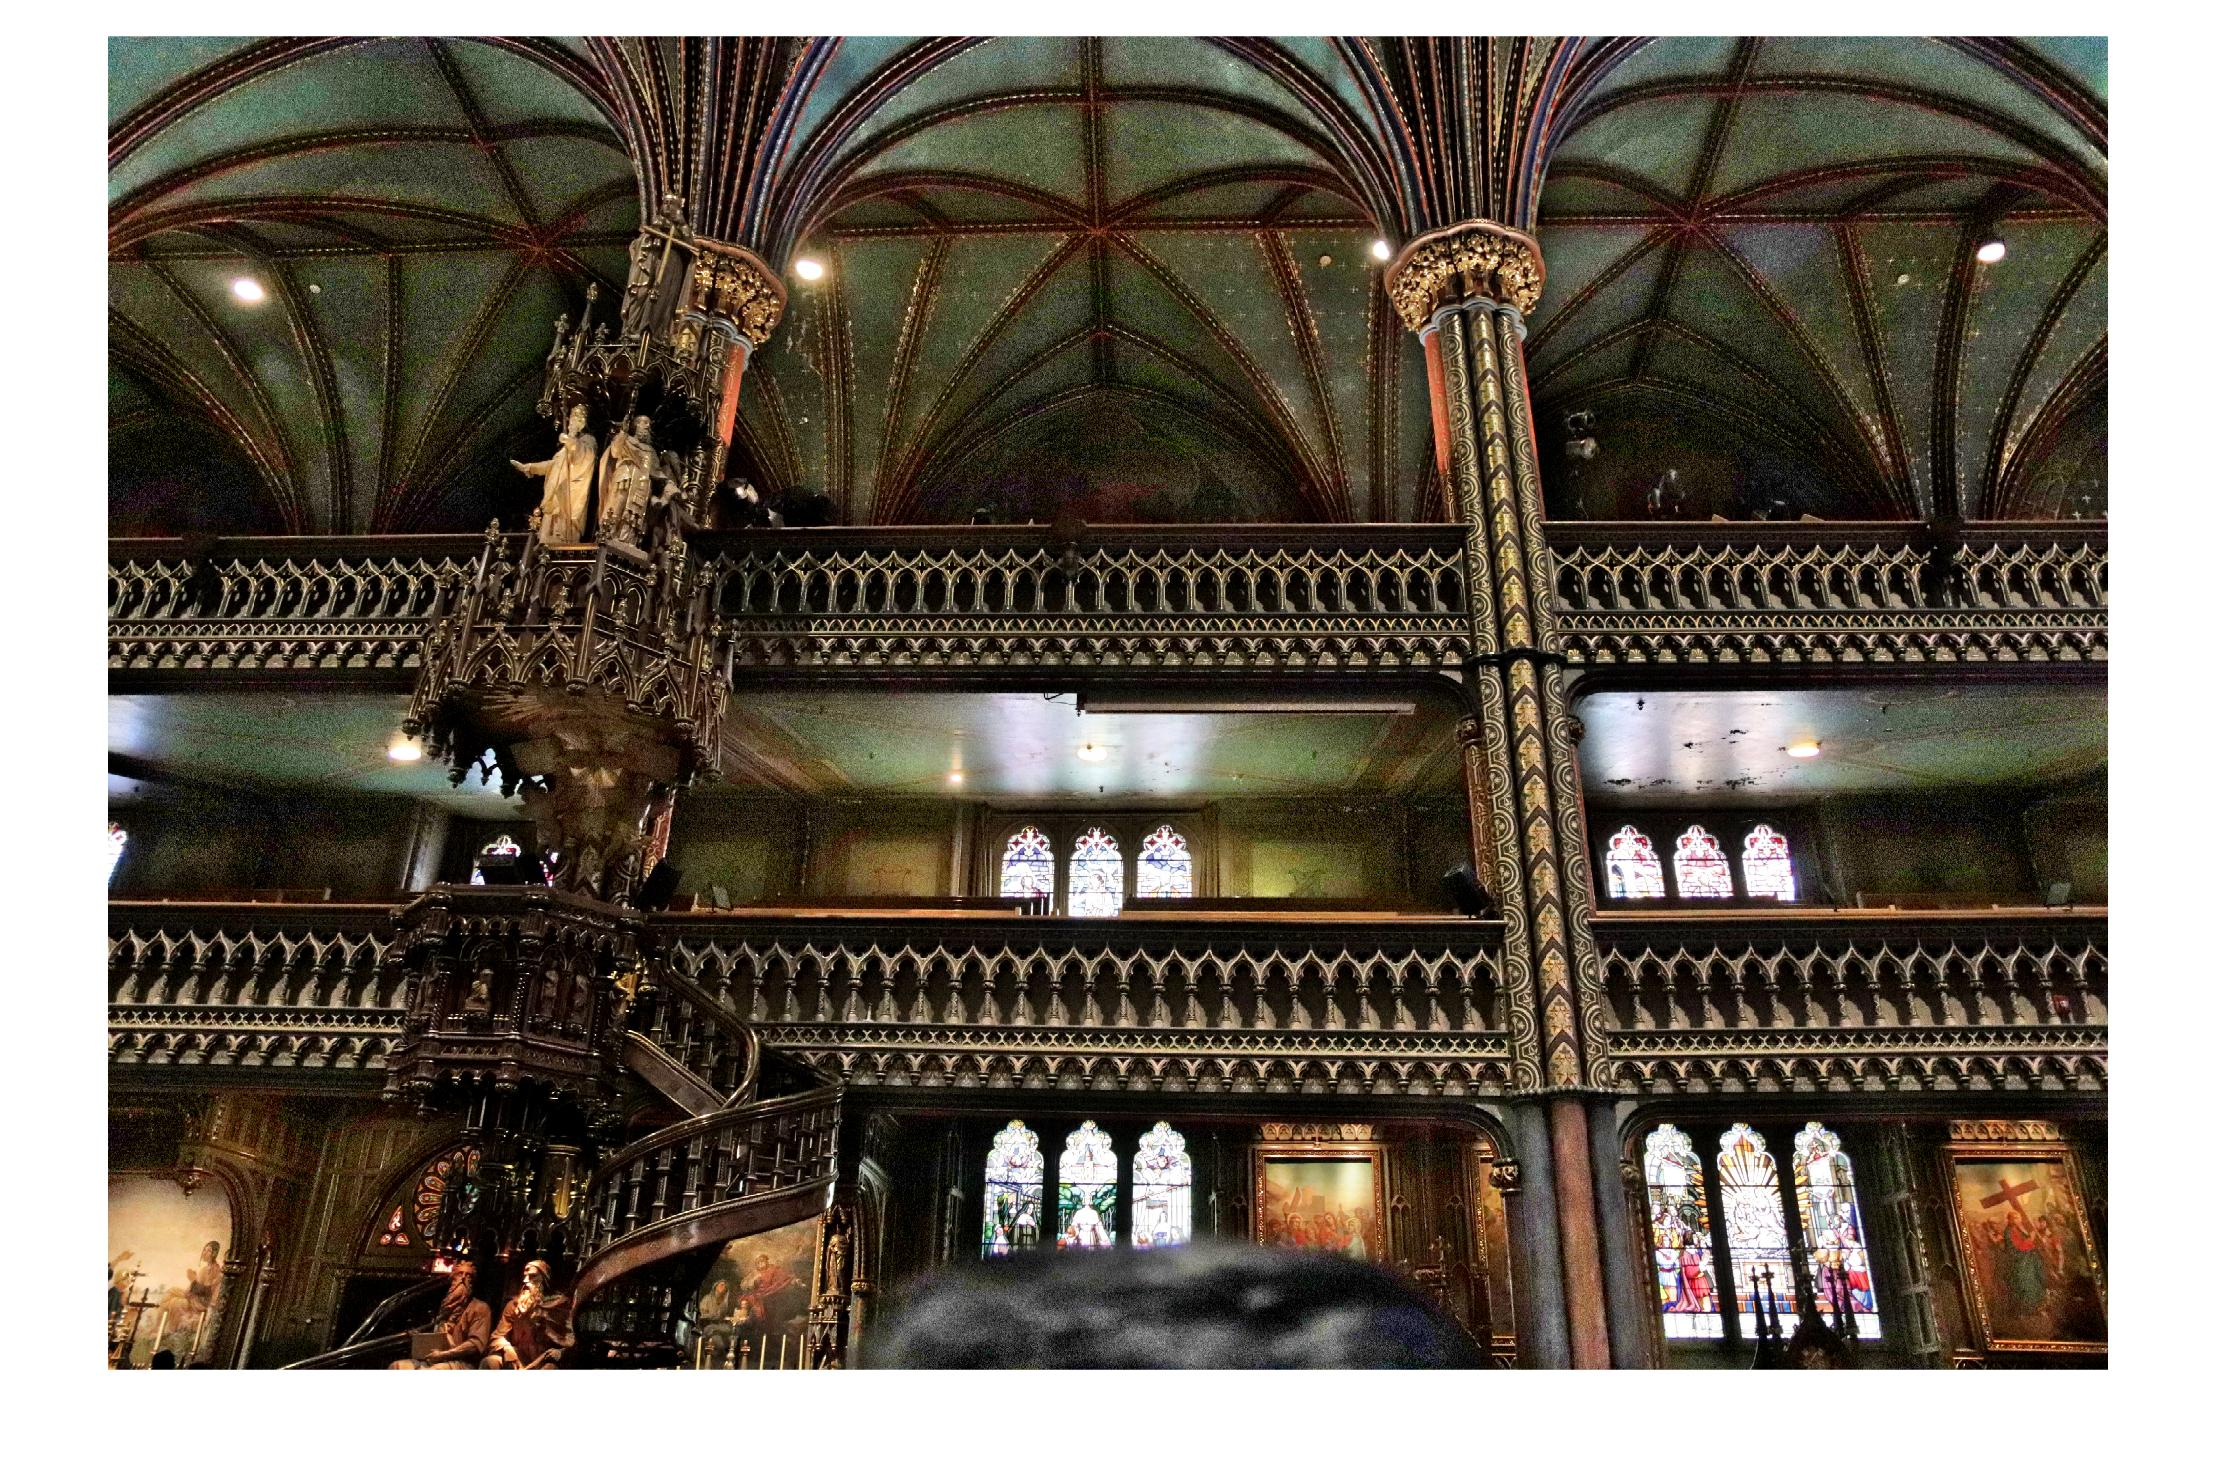
\includegraphics[width=\linewidth]{images/img25.jpg}
\caption{Improve image}
\end{subfigure}
\caption{Improve results further using 'imreducehaze' optional parameters}
\label{fig:Improvement}
\end{figure}

\subsection{Improve Results Using Denoising}

\begin{lstlisting}[language=Matlab]

% Improve Results Using Denoising
% Use the imguidedfilter function 
to remove noise from the enhanced image
denoised_img = imguidedfilter(improved_img);
figure;
imshow(denoised_img);

\end{lstlisting}

\begin{figure}[h!]
\centering
\begin{subfigure}[b]{0.4\linewidth}
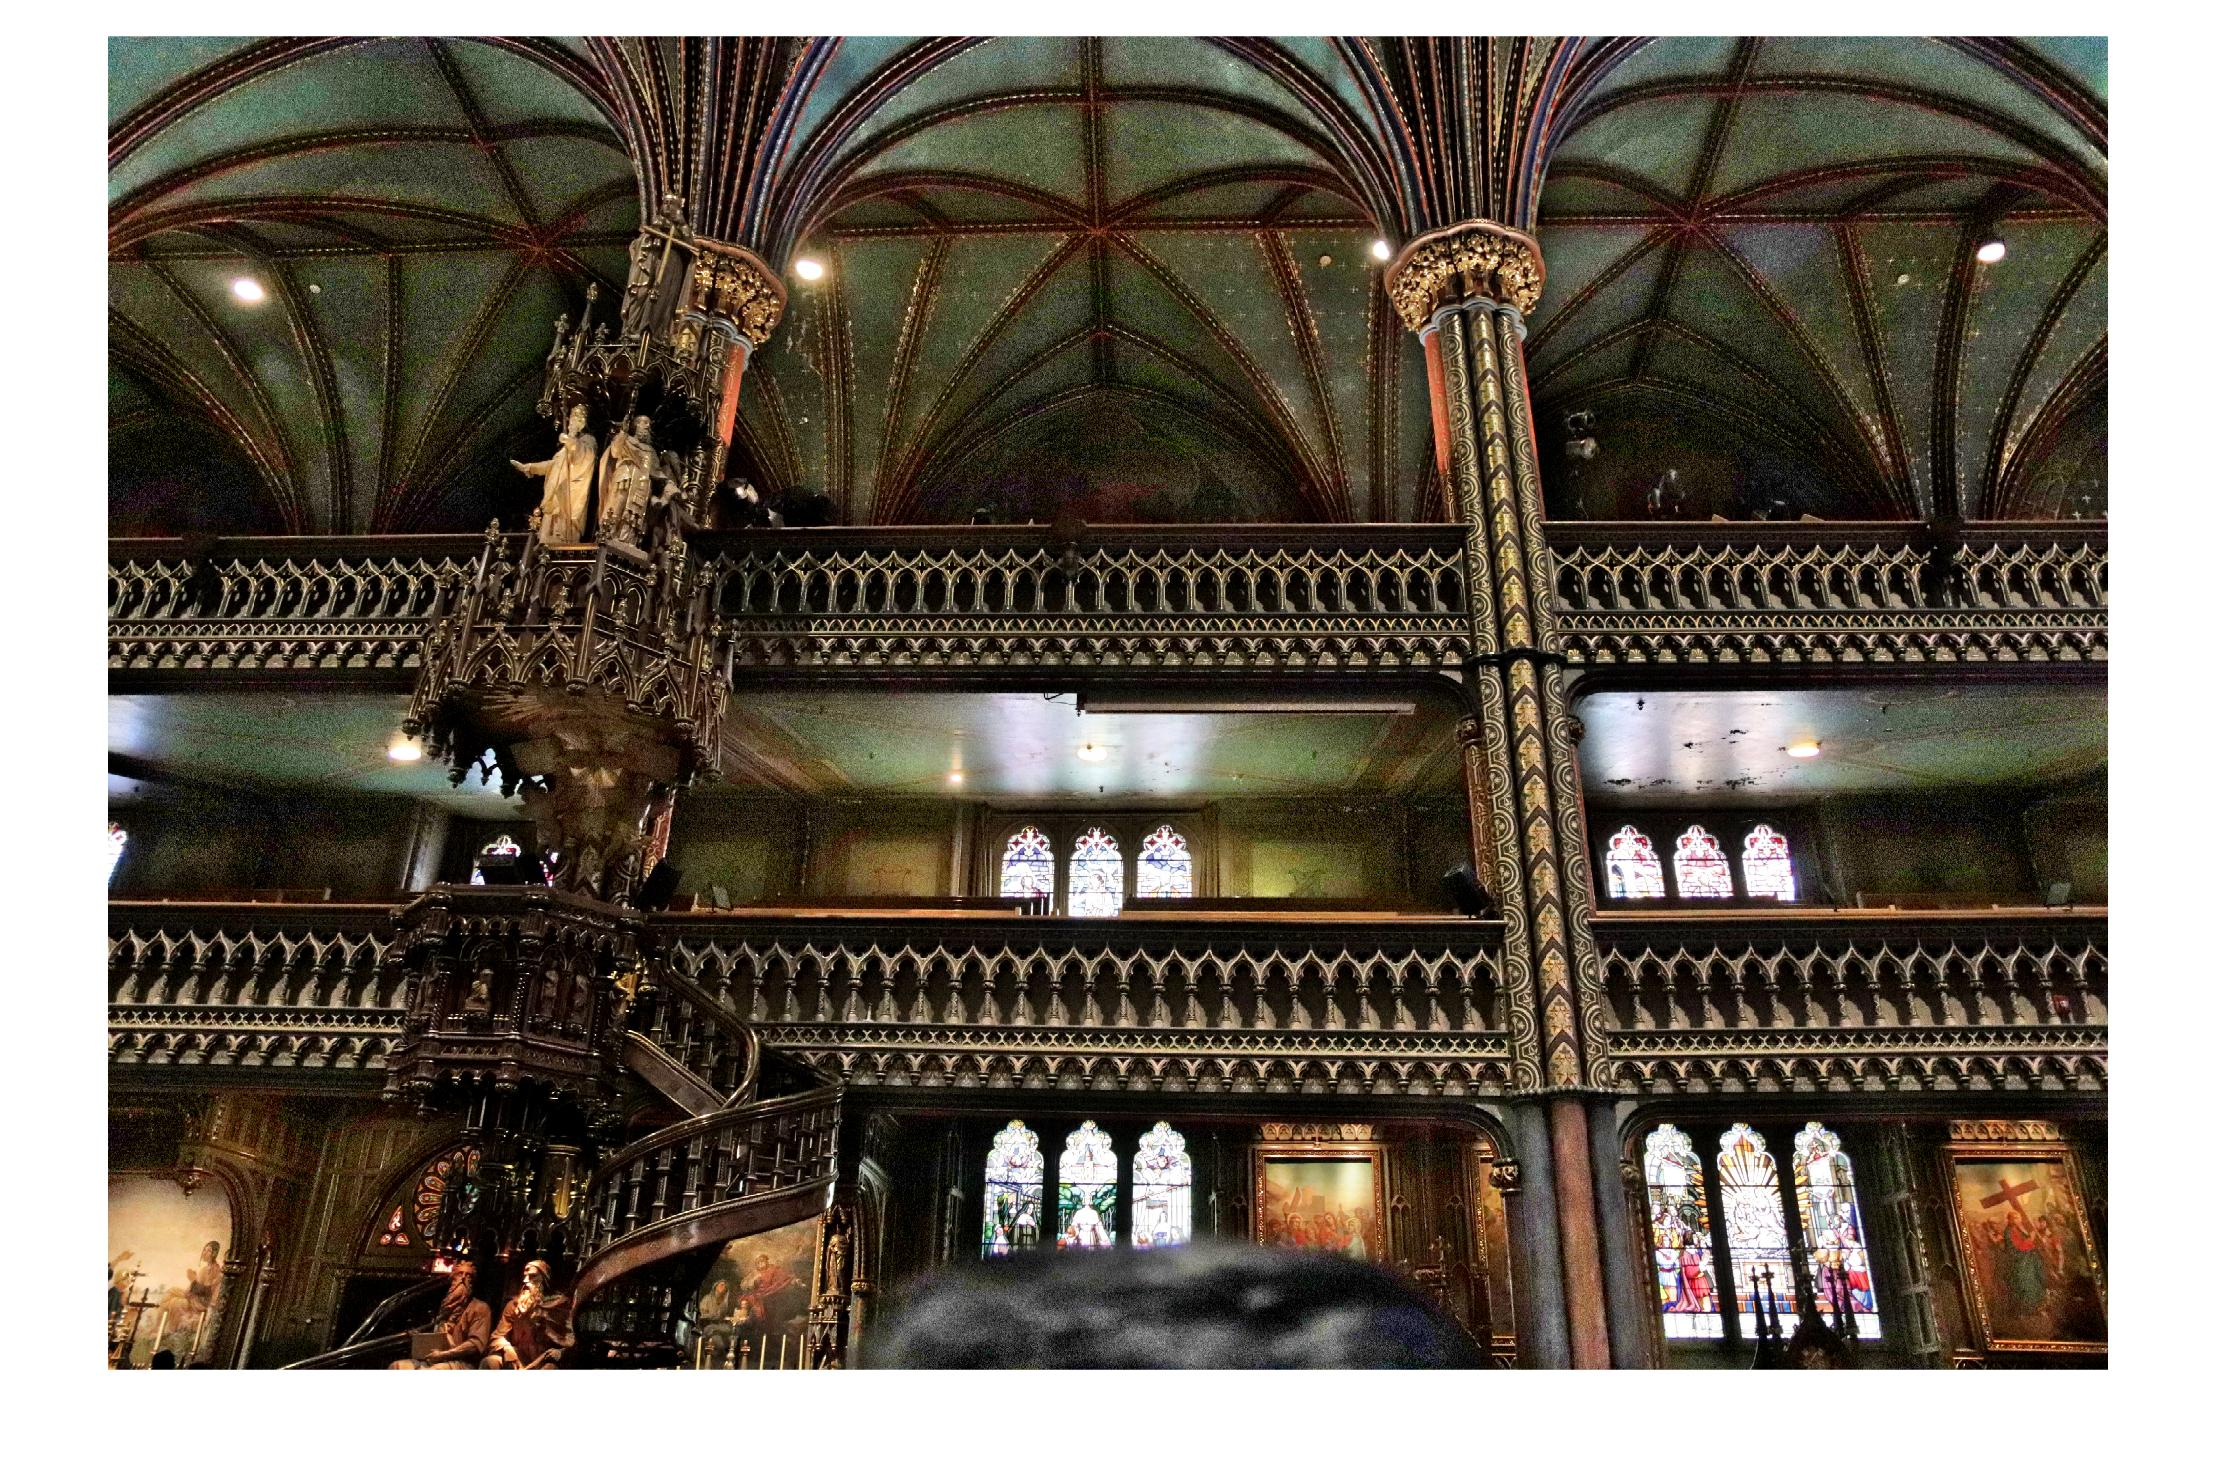
\includegraphics[width=\linewidth]{images/img25.jpg}
\caption{Improved image}
\end{subfigure}
\begin{subfigure}[b]{0.4\linewidth}
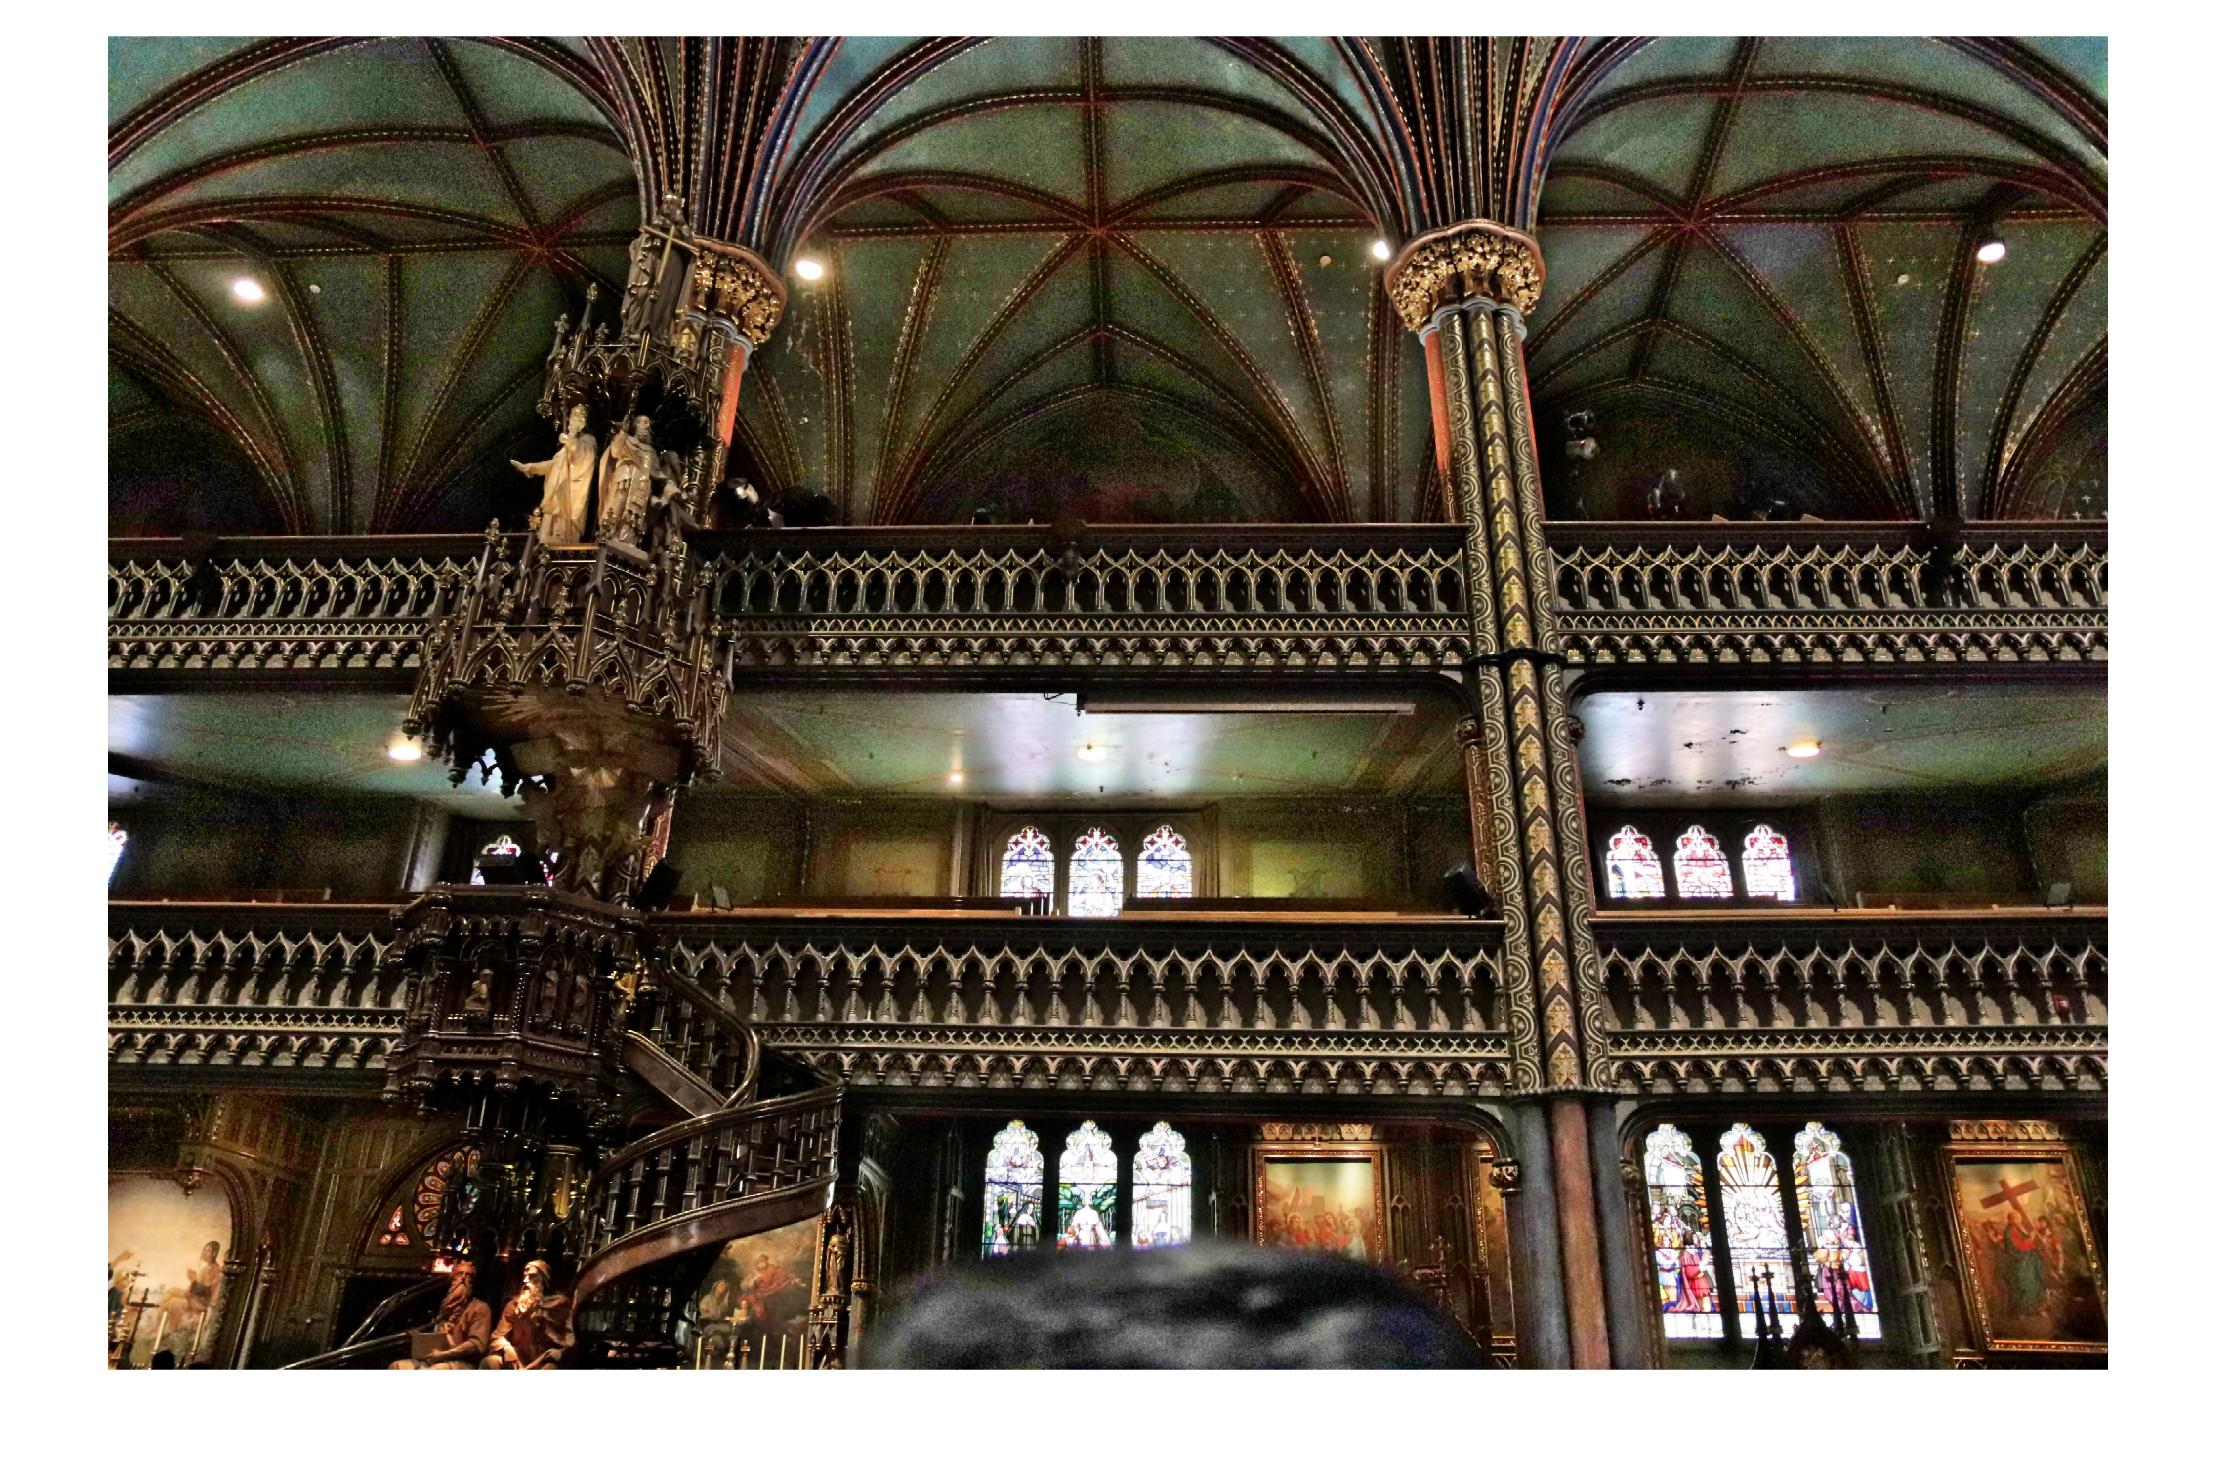
\includegraphics[width=\linewidth]{images/img26.jpg}
\caption{Denoised image}
\end{subfigure}
\caption{Improve results using denoising}
\label{fig:Denoising}
\end{figure}

\subsection{Another Example of Improving Poorly Lit Image}

\begin{lstlisting}[language=Matlab]

% Assignment 2
% Part 2

% Import an RGB image 
%captured in low light
img = imread('/lamnguyen/Desktop/School/
Computer-Vision/A2/images/church2.jpg');
img = imrotate(img, 90);
figure; 
imshow(img);

% Invert the image and 
% notice how the low-light
% areas in the original image appear hazy
inverted_img = imcomplement(img);

% Reduce the haze 
reduced_img = imreducehaze(inverted_img, 
'ContrastEnhancement', 'none');

% Invert the results to 
% obtain the enhanced image
enhanced_img = imcomplement(reduced_img);
figure;
imshow(enhanced_img);

\end{lstlisting}

\begin{figure}[h!]
\centering
\begin{subfigure}[b]{0.4\linewidth}
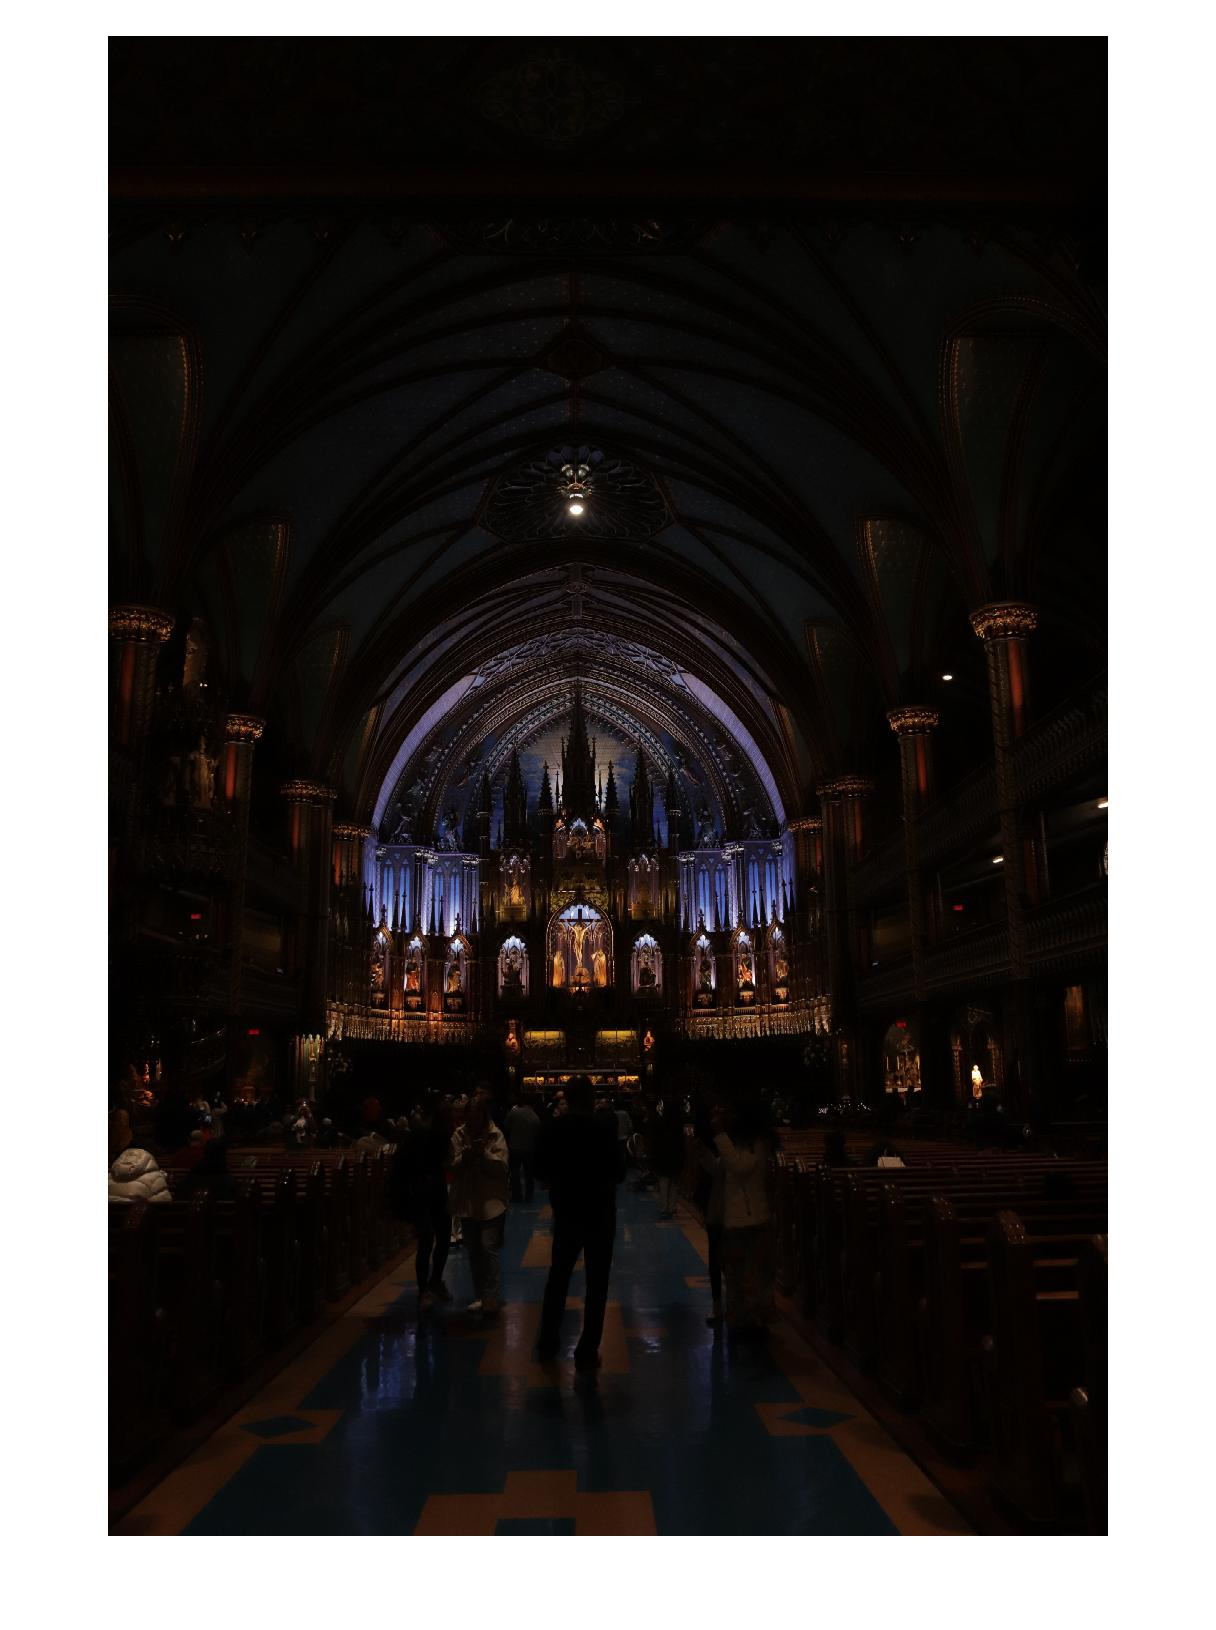
\includegraphics[width=\linewidth]{images/img27.jpg}
\caption{Original image}
\end{subfigure}
\begin{subfigure}[b]{0.4\linewidth}
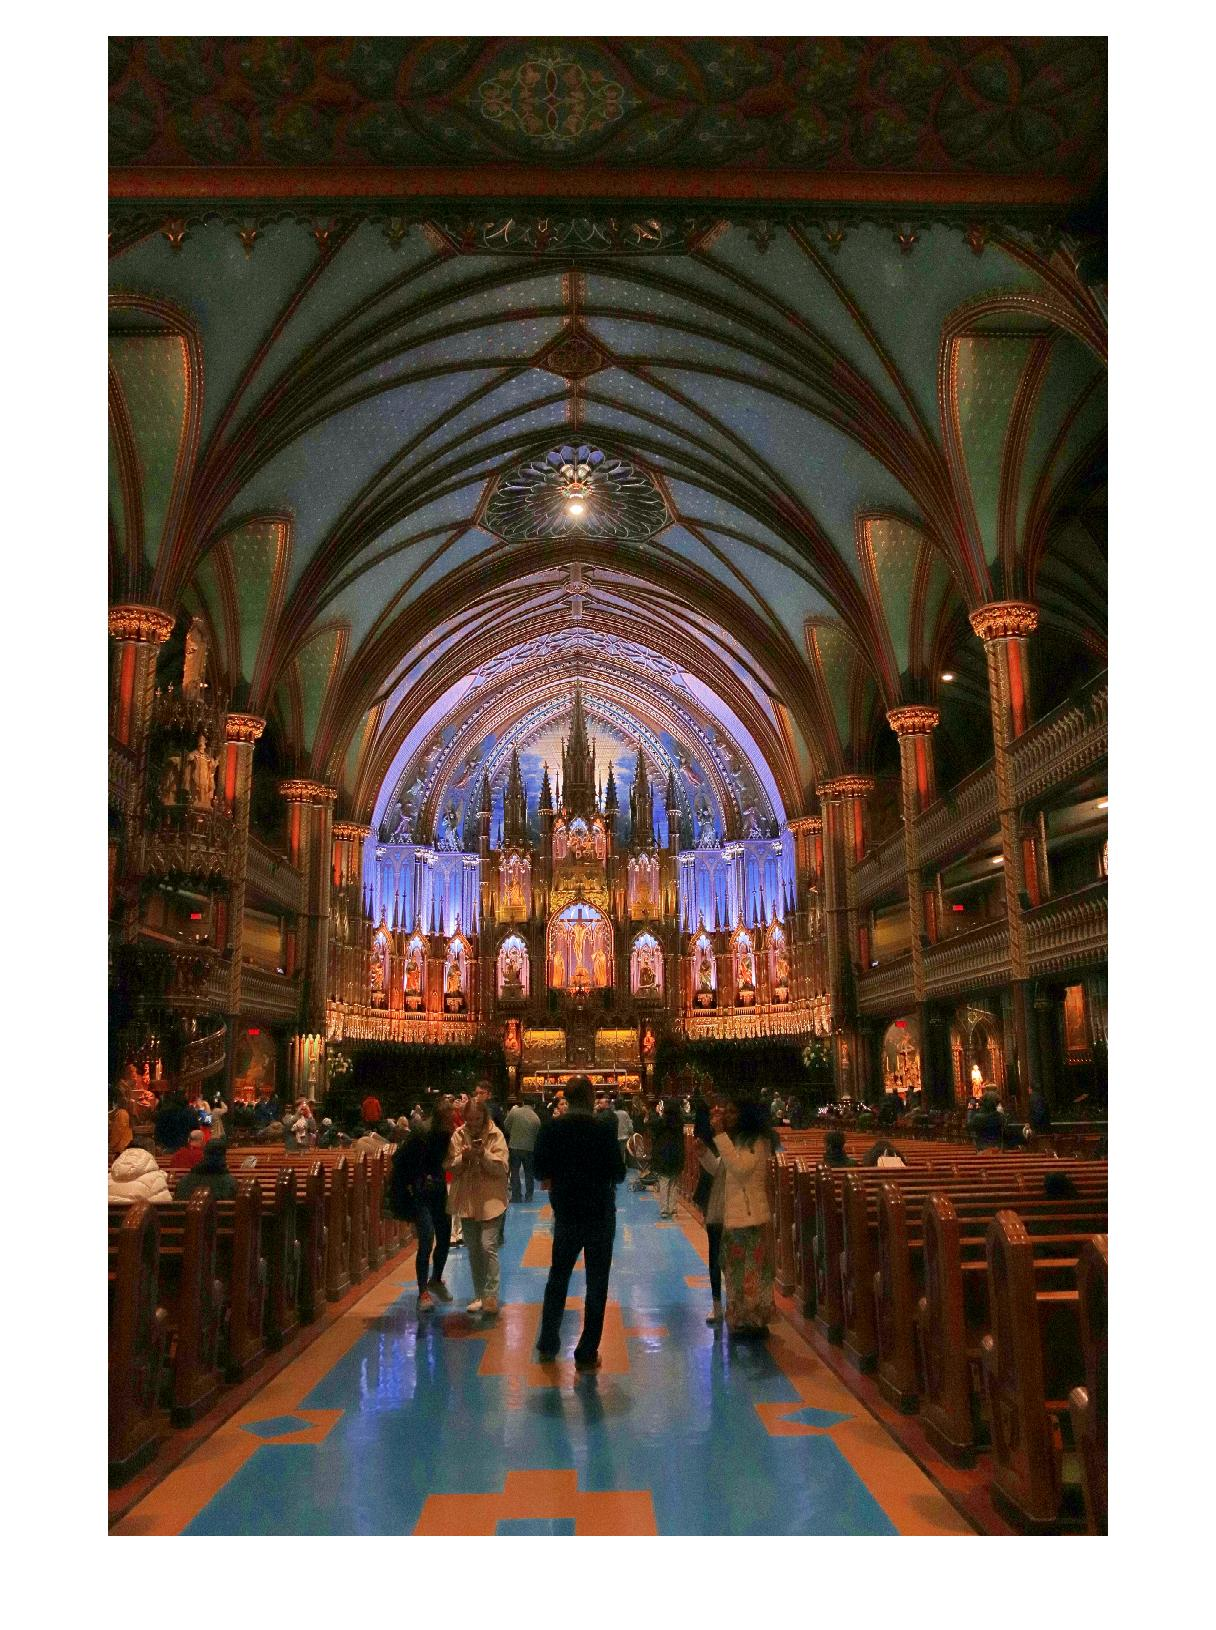
\includegraphics[width=\linewidth]{images/img28.jpg}
\caption{Enhanced image}
\end{subfigure}
\caption{Another example of improving poorly lit image}
\label{fig:example}
\end{figure}

\subsection{Reduce Color Distortion by Using Different Color Space}

\begin{lstlisting}[language=Matlab]

% Convert the input image from the RGB 
% colorspace to the L*a*b* colorspace
Lab = rgb2lab(img);
% Invert the L*a*b* image
LInv = imcomplement(Lab(:,:,1) ./ 100);
% Dehaze the inverted image using 
% the imreducehaze function
LEnh = imcomplement(imreducehaze
(LInv,'ContrastEnhancement','none'));
% Increase the saturation
LabEnh(:,:,1)   = LEnh .* 100;
LabEnh(:,:,2:3) = Lab(:,:,2:3) * 2; 
% Convert the image back to an RGB image
AEnh = lab2rgb(LabEnh);
figure;
imshow(AEnh);

\end{lstlisting}

\begin{figure}[h!]
\centering
\begin{subfigure}[b]{0.4\linewidth}
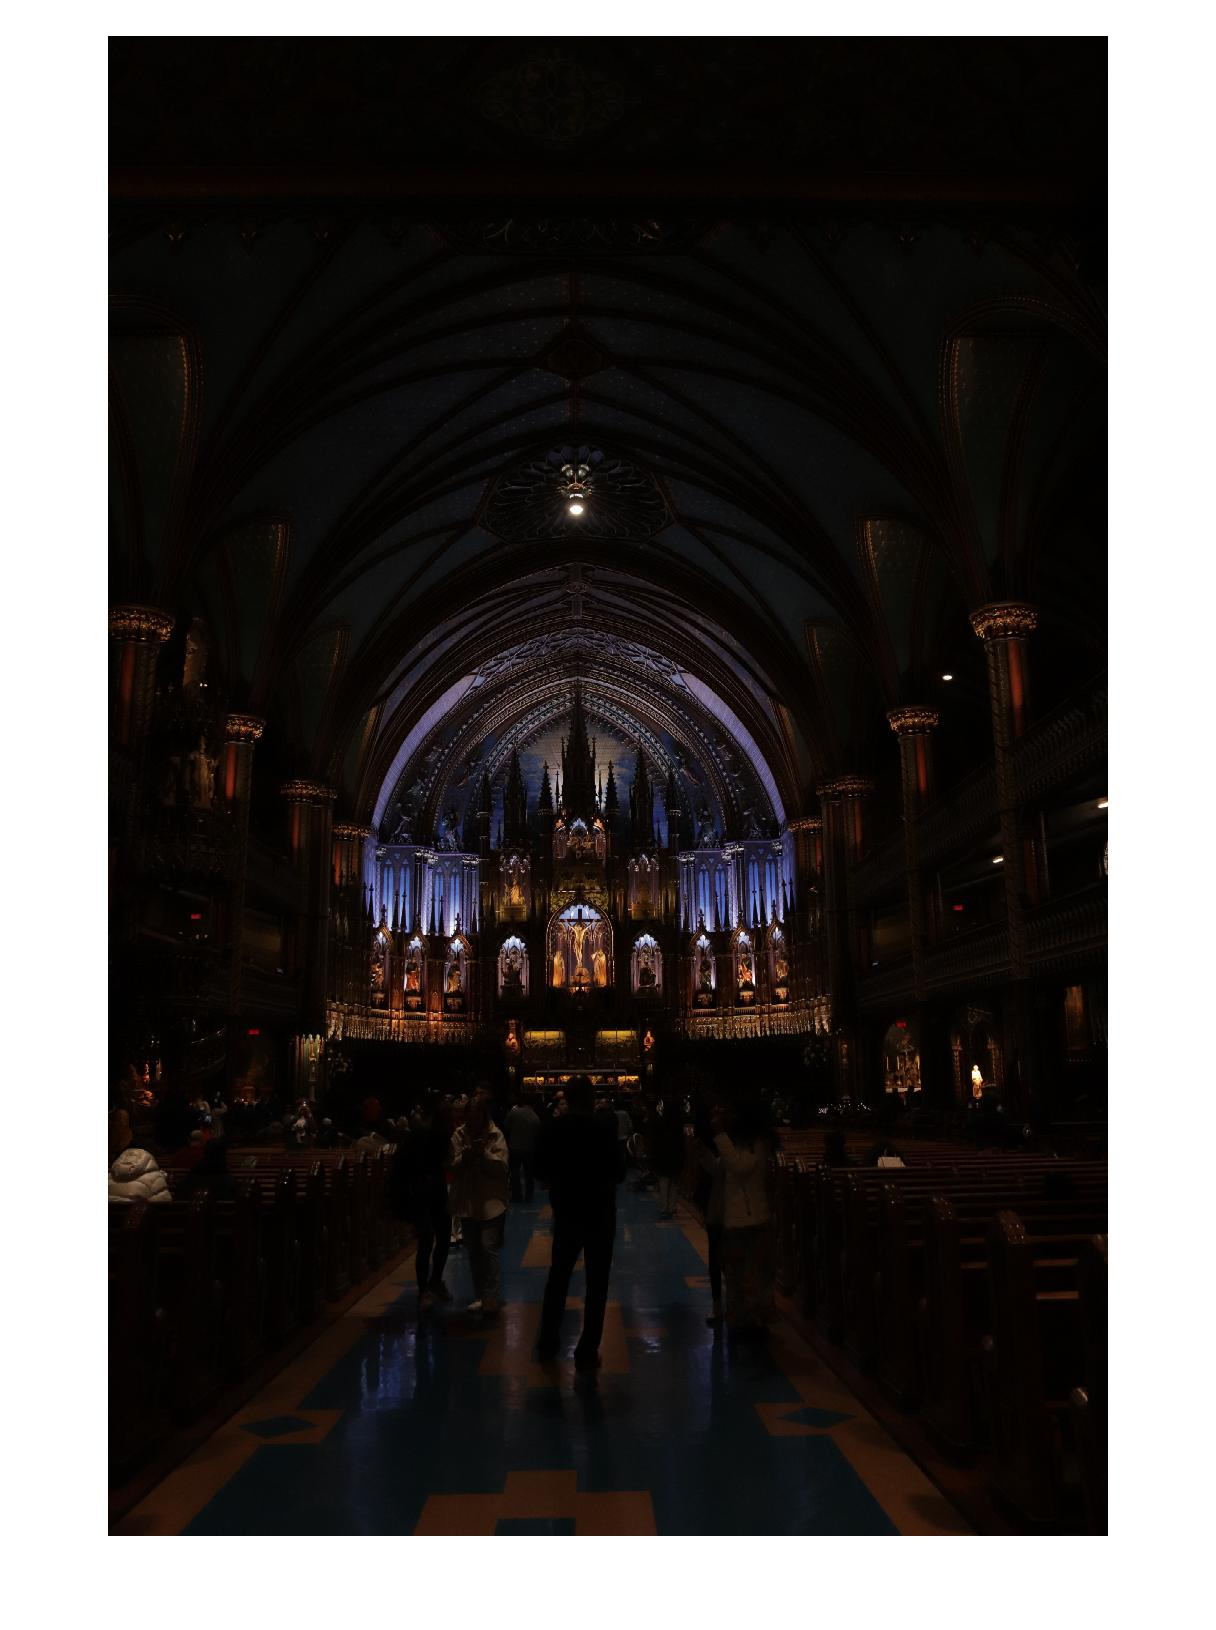
\includegraphics[width=\linewidth]{images/img27.jpg}
\caption{Original image}
\end{subfigure}
\begin{subfigure}[b]{0.4\linewidth}
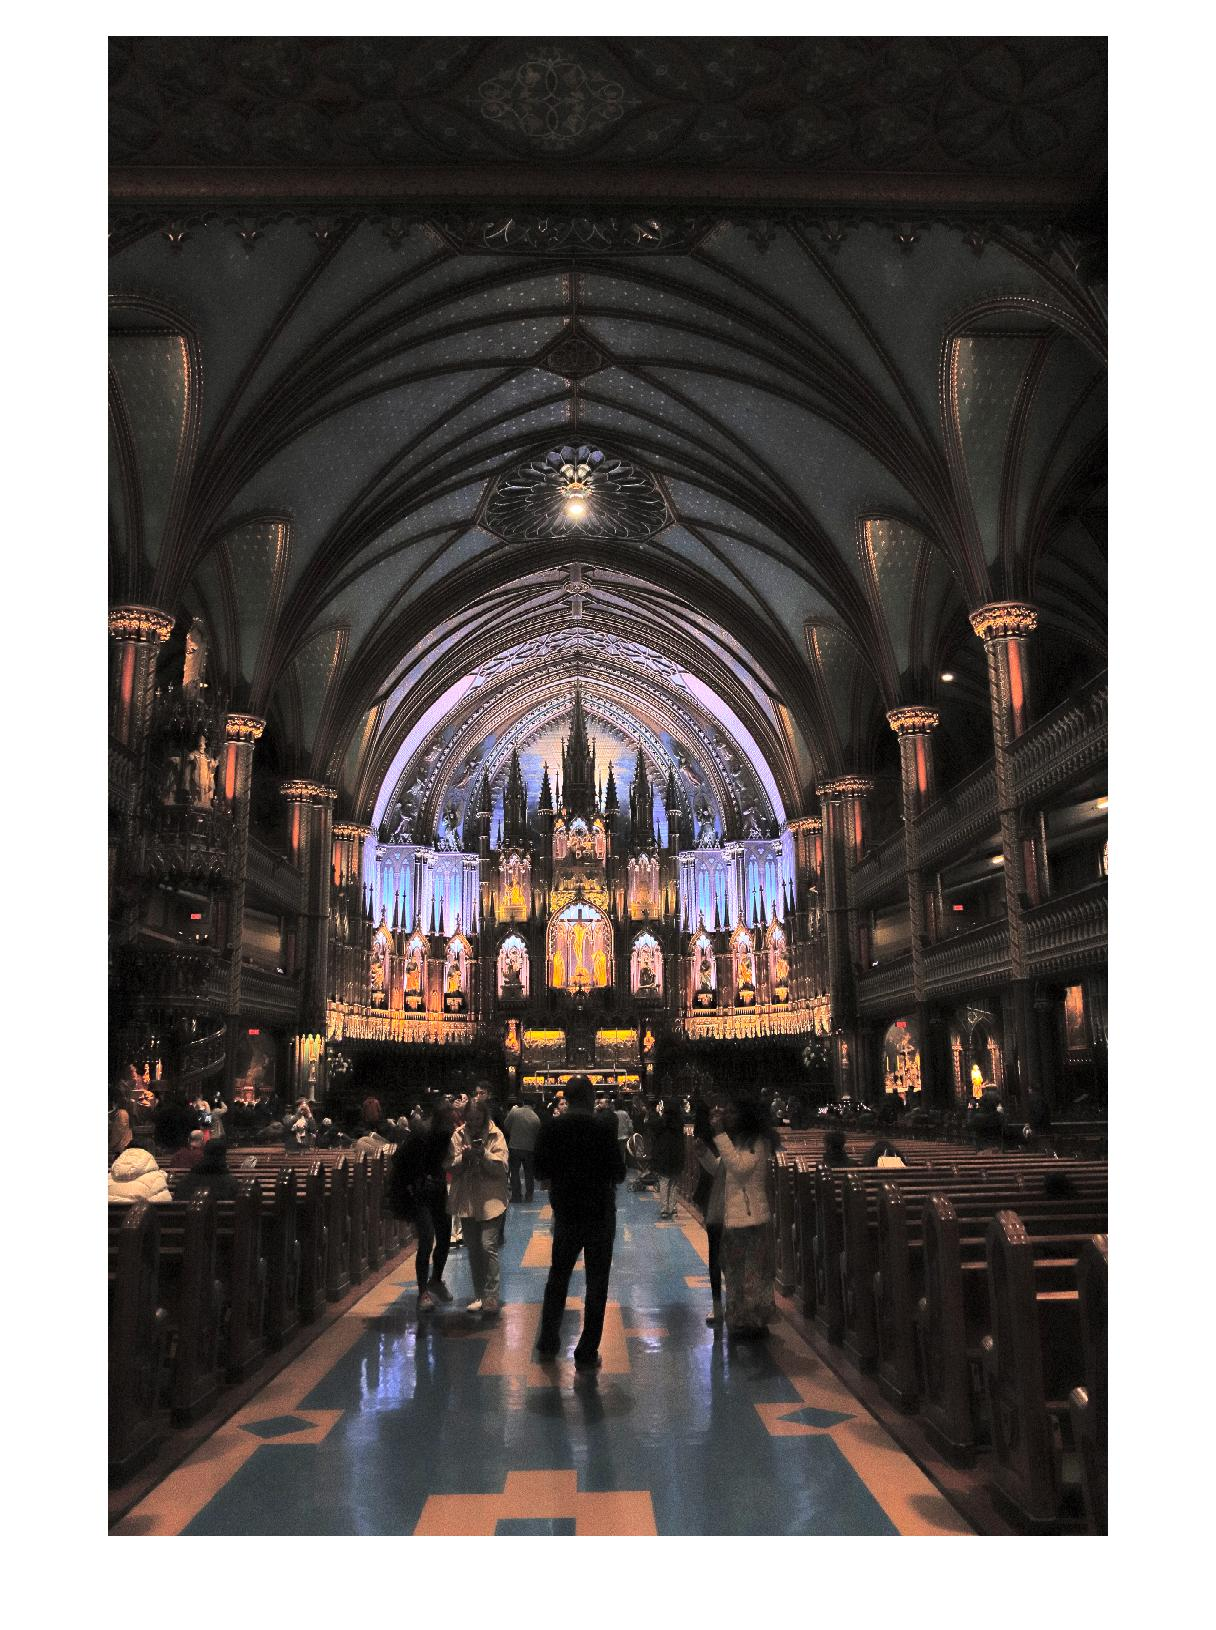
\includegraphics[width=\linewidth]{images/img29.jpg}
\caption{Enhanced image}
\end{subfigure}
\caption{Reduce color distortion by using different color space}
\label{fig:Lab}
\end{figure}

\subsection{Estimate Illumination Map}

\begin{lstlisting}[language=Matlab]

% Apply the dehazing 
%algorithm to the image
[BInv,TInv] = imreducehaze(inverted_img,
'Method','approxdcp','ContrastEnhancement', 
'none');

% Invert the enhanced image
T = imcomplement(TInv);
figure;
imshow(T)
colormap(hot)

\end{lstlisting}

\begin{figure}[h!]
\centering
\begin{subfigure}[b]{0.4\linewidth}
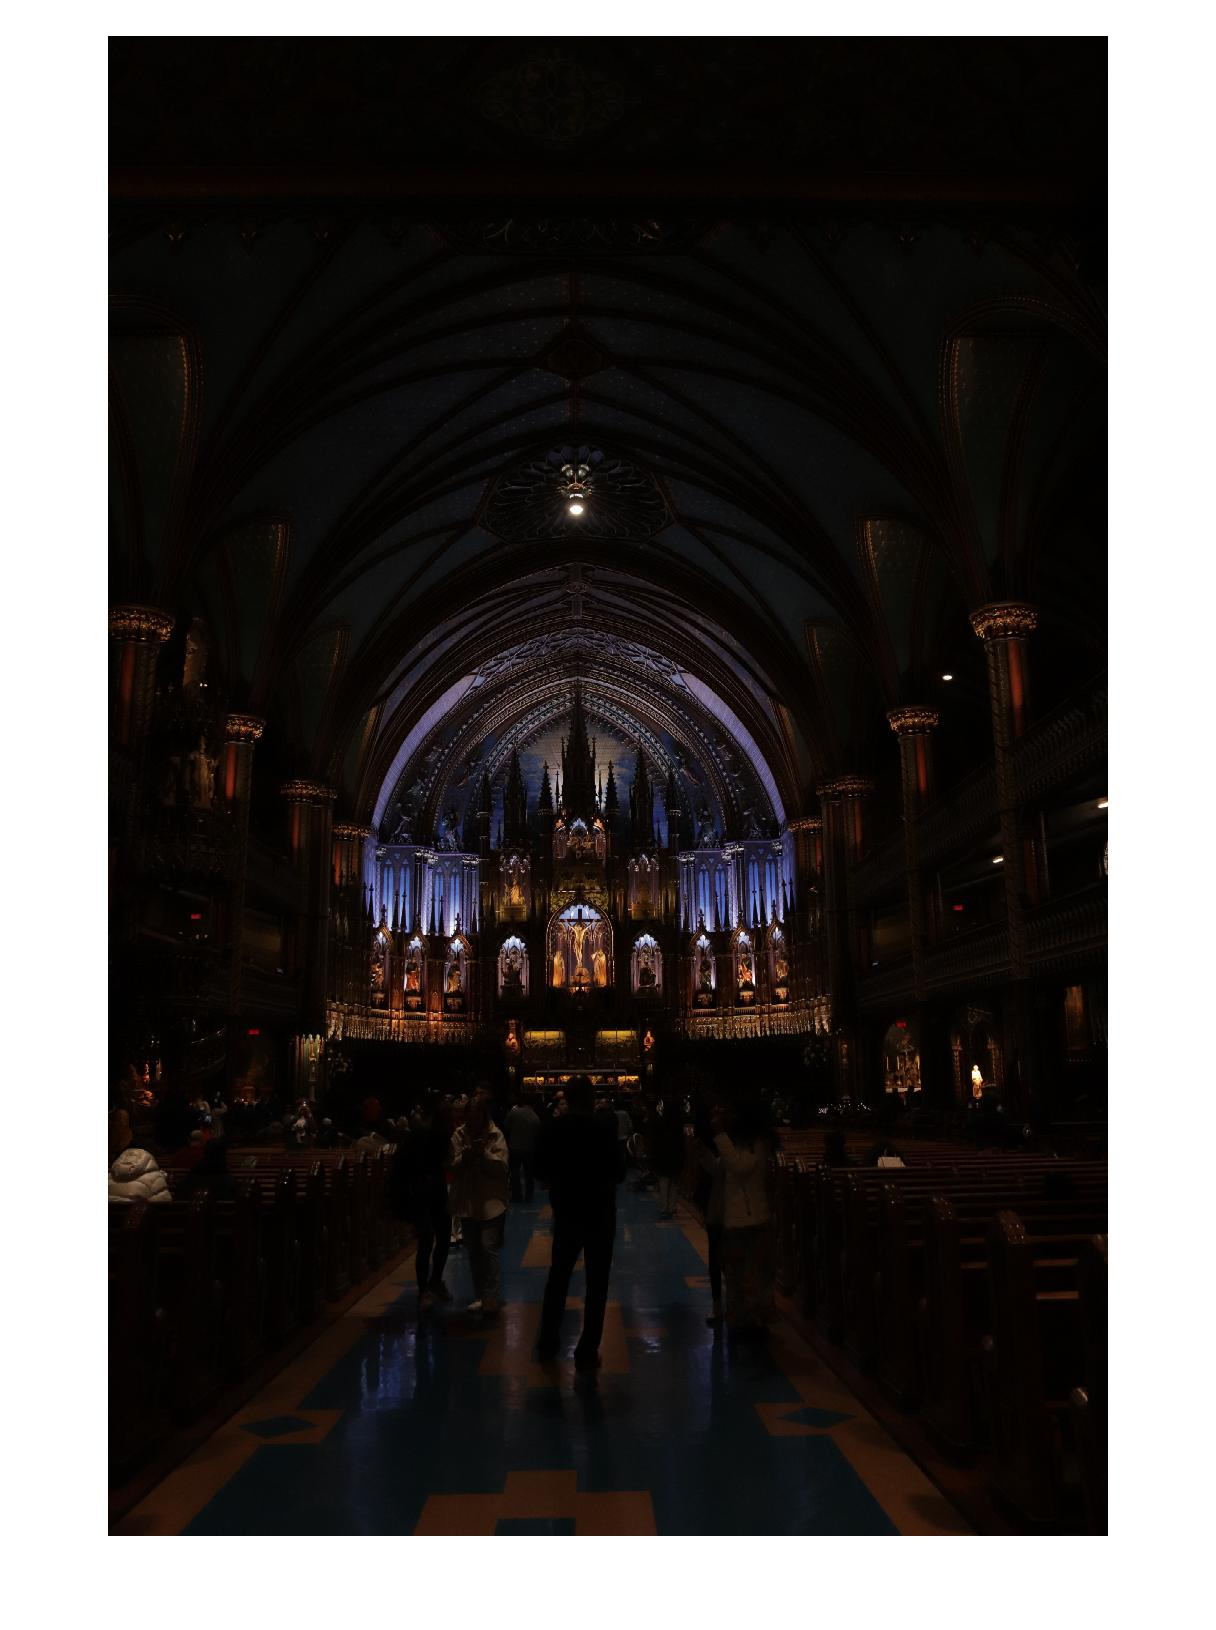
\includegraphics[width=\linewidth]{images/img27.jpg}
\caption{Original image}
\end{subfigure}
\begin{subfigure}[b]{0.4\linewidth}
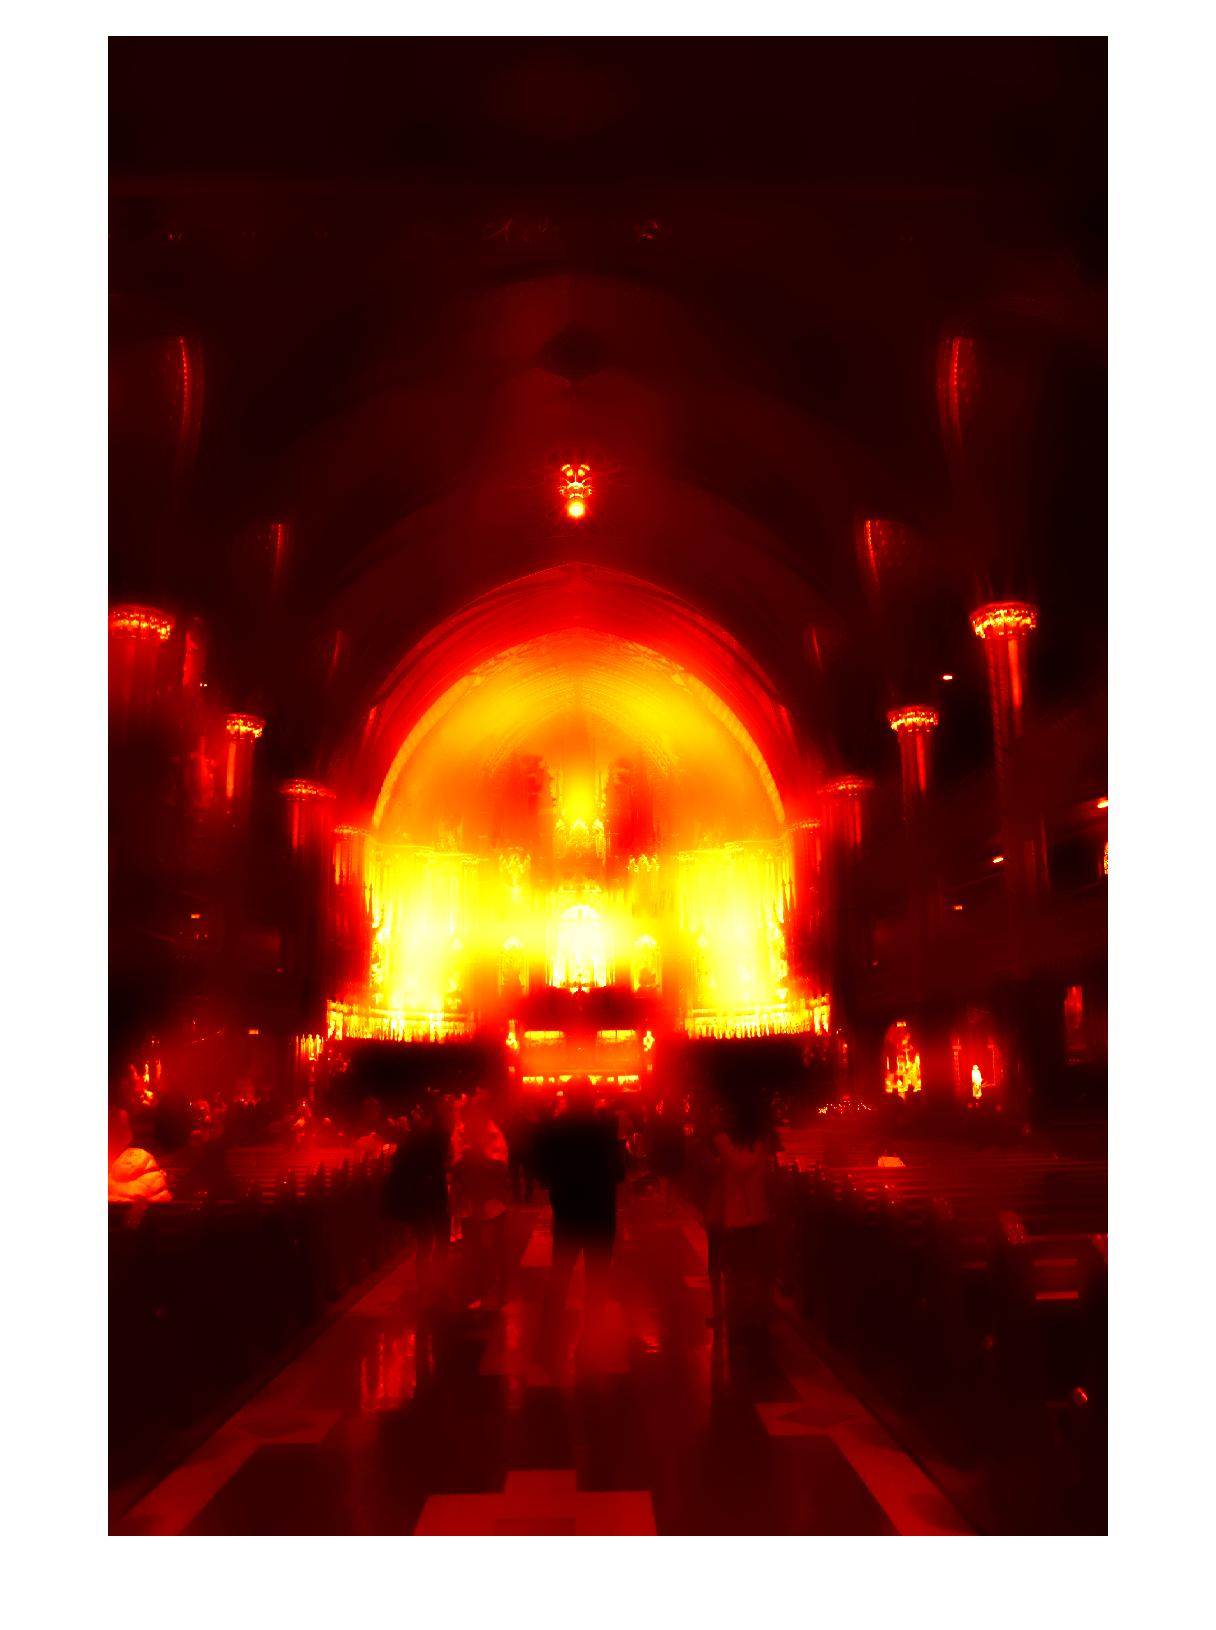
\includegraphics[width=\linewidth]{images/img30.jpg}
\caption{Illumination map}
\end{subfigure}
\caption{Estimate illumination map}
\label{fig:illumination map}
\end{figure}



\section{Part 3}

The tentative topic for final project is handwriting recognition. 

\end{document}
